\chapter{Exploration Analytics Methodology}\label{ch3:expl_methods}

\section{Exploration Data Sources}\label{ch3:expl_data_src}

This investigation brings together a total of twenty-five (25) data sets covering the southwest NM study area. Data were collected from previously published works, open-access databases, or derived from those original sources as secondary products. The form of the data varies between pre-gridded raster files, point data sets with repeat or overlapping measurements, non-overlapping point sets, and line data. Previous researchers created raster files or raster-ready gridded data for nine of the features. Four are generated by running procedures on one of the existing rasters. The remaining layers were created from polylines (3), overlapping points (4), and non-overlapping points (2). Although complex interactions between earth systems should be expected, these layers represent the independent variables for analysis purposes. Section XXX details how evaluating collinearities between features allows for pre-screening before modeling, and further analysis of feature importances helps reduce this composite data set to a smaller subset for simpler prediction models.

\begin{table}[htp]
\centering
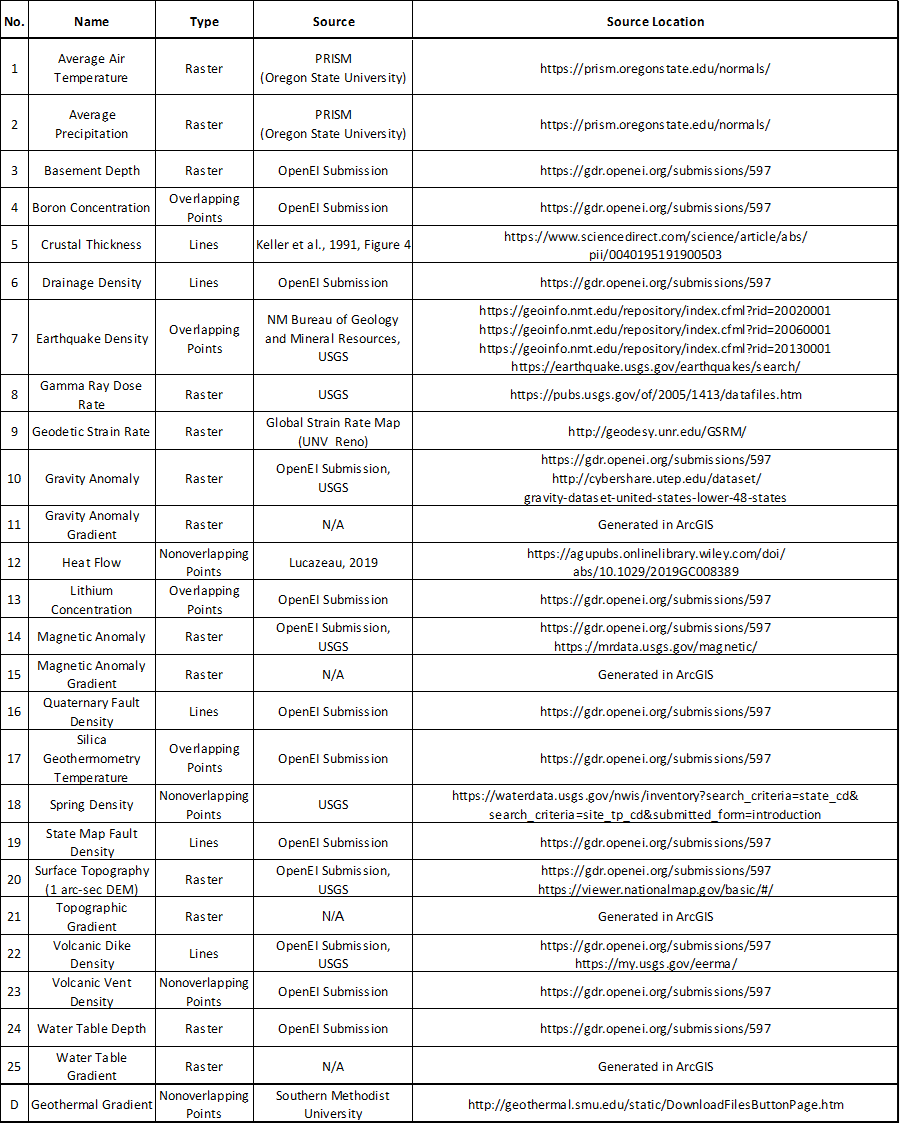
\includegraphics[scale=1]{Table-Features.png}
\caption[Features considered in this the exploration analytics study]{List of data sets considered in this study. Data type, provider, and source location are listed. Numbered features are treated as independent variables. 'D' indicates the dependent variable.}
\label{tab:features}
\end{table}

As discussed in Section \ref{ch2:sysfund}, geothermal systems require permeability, heat, subsurface fluids, a trapping mechanism, and recharge. Following the slightly more simplified PFA assumptions of \citeauthor{bielicki_hydrogeolgic_2015} (\citeyear{bielicki_hydrogeolgic_2015}), an explorationist will want to quickly identify where heat, permeability, and fluids together define a favorable setting for a geothermal prospect. The prepared independent data inputs collectively address all three elements as noted in Table \ref{tab:features}. Rather than defining a dependent (predicted) variable that describes a total favorability score, this thesis focuses on a proof of concept prediction for a measurable quantity addressing just the heat risk element: geothermal gradient. This choice was made because a) geothermal gradient provides a direct proxy for accessible heat content, b) gradient point data is available from suitable compilations of well measurements collected across the study area, and c) for EGS applications, the only risk element that must be naturally present is heat. Heat flow might be a reasonable alternative dependent variable, however point values for heat flow in the available well database were derived directly from geothermal gradient values. Geothermometer measurements also suggest resource temperatures, but the uncertainty in fluid pathways leading to the sample location means these values suffer from less spatial and depth certainty than geothermal gradient.

Regarding the remaining two risk elements: direct measurements of permeability (i.e., from downhole logs or core analysis) or fluids (e.g., flow rate from well tests) can be separately predicted using the same methods described in this study. A final favorability score, which is less straight-forward to calibrate for model validation and verification, could potentially be derived from the combined predictions as done in PFA risk assessments. This suggestion is outside of the scope of this thesis and thus appears in the list of future work opportunities (see Chapter 9).

\section{Exploration Data Preparation}

In order to experiment with a variety of machine learning methods, all input data sets first need to be transformed into fully-complete \acrlong{gis} (\acrshort{gis}) layers such that any point on the map of the study area has a corresponding set of 25 independent feature values. Steps taken to condition, process, and otherwise prepare each layer are outlined later in this chapter. As a preface, the following section reviews several key algorithms and concepts applied to one or more of the layers for clarity and reproducibility.

\subsection{Data Preparation Algorithms}

\subsubsection{Extents}

Large data sets imported into ArcGIS or Python for feature preparation required cropping to the southwest New Mexico study area. Two polygons were used for this purpose:

\begin{itemize}
\item Extent Polygon: this is a simple rectangular polygon capturing the broader southwestern NM region. It is defined by the following corner points in degrees N Latitude and degrees E Longitude: \\ (-31.3, -109.1), (31.3, -105.9), (35.4, -105.9), (31.3, -109.1)
\item \acrlong{aoi} (\acrshort{aoi}): this polygon appears in most map figures in this thesis and is the perimeter outlining the nine counties in Southwest New Mexico: Cibola, Valencia, Catron, Socorro, Grant, Sierra, Luna, Dona Ana, and Hidalgo.
\end{itemize}

\subsubsection{Fishnet Points}\label{ssn:fishnet}

\subsubsection{Simple Kriging}\label{ssn:kriging}

\subsubsection{Empirical Bayes Kriging}\label{ssn:ebk}

\subsubsection{Splines}

\subsubsection{Topo to Raster?}

\subsubsection{\acrlong{kde} (\acrshort{kde})}\label{ssn:kde}

\subsection{Data Layers}

\subsubsection{Average Air Temperature}

The University of Oregon PRISM Climate Group hosts regularly-updated spatial data sets of climate-related observations captured from different monitoring networks, including 30-year normals that describe average monthly or annual conditions \citep{daly_physiographically_2008, prism_prism_2021}. 800 m or 4 km resolution grids can be accessed directly from the website. The 800 m resolution air temperature grid was downloaded and imported into ArcGIS, then cropped using the Extent Polygon (Figure \ref{fig:feat_airtemp}). The layer required no further processing.

\begin{figure}[!htp]
\centering
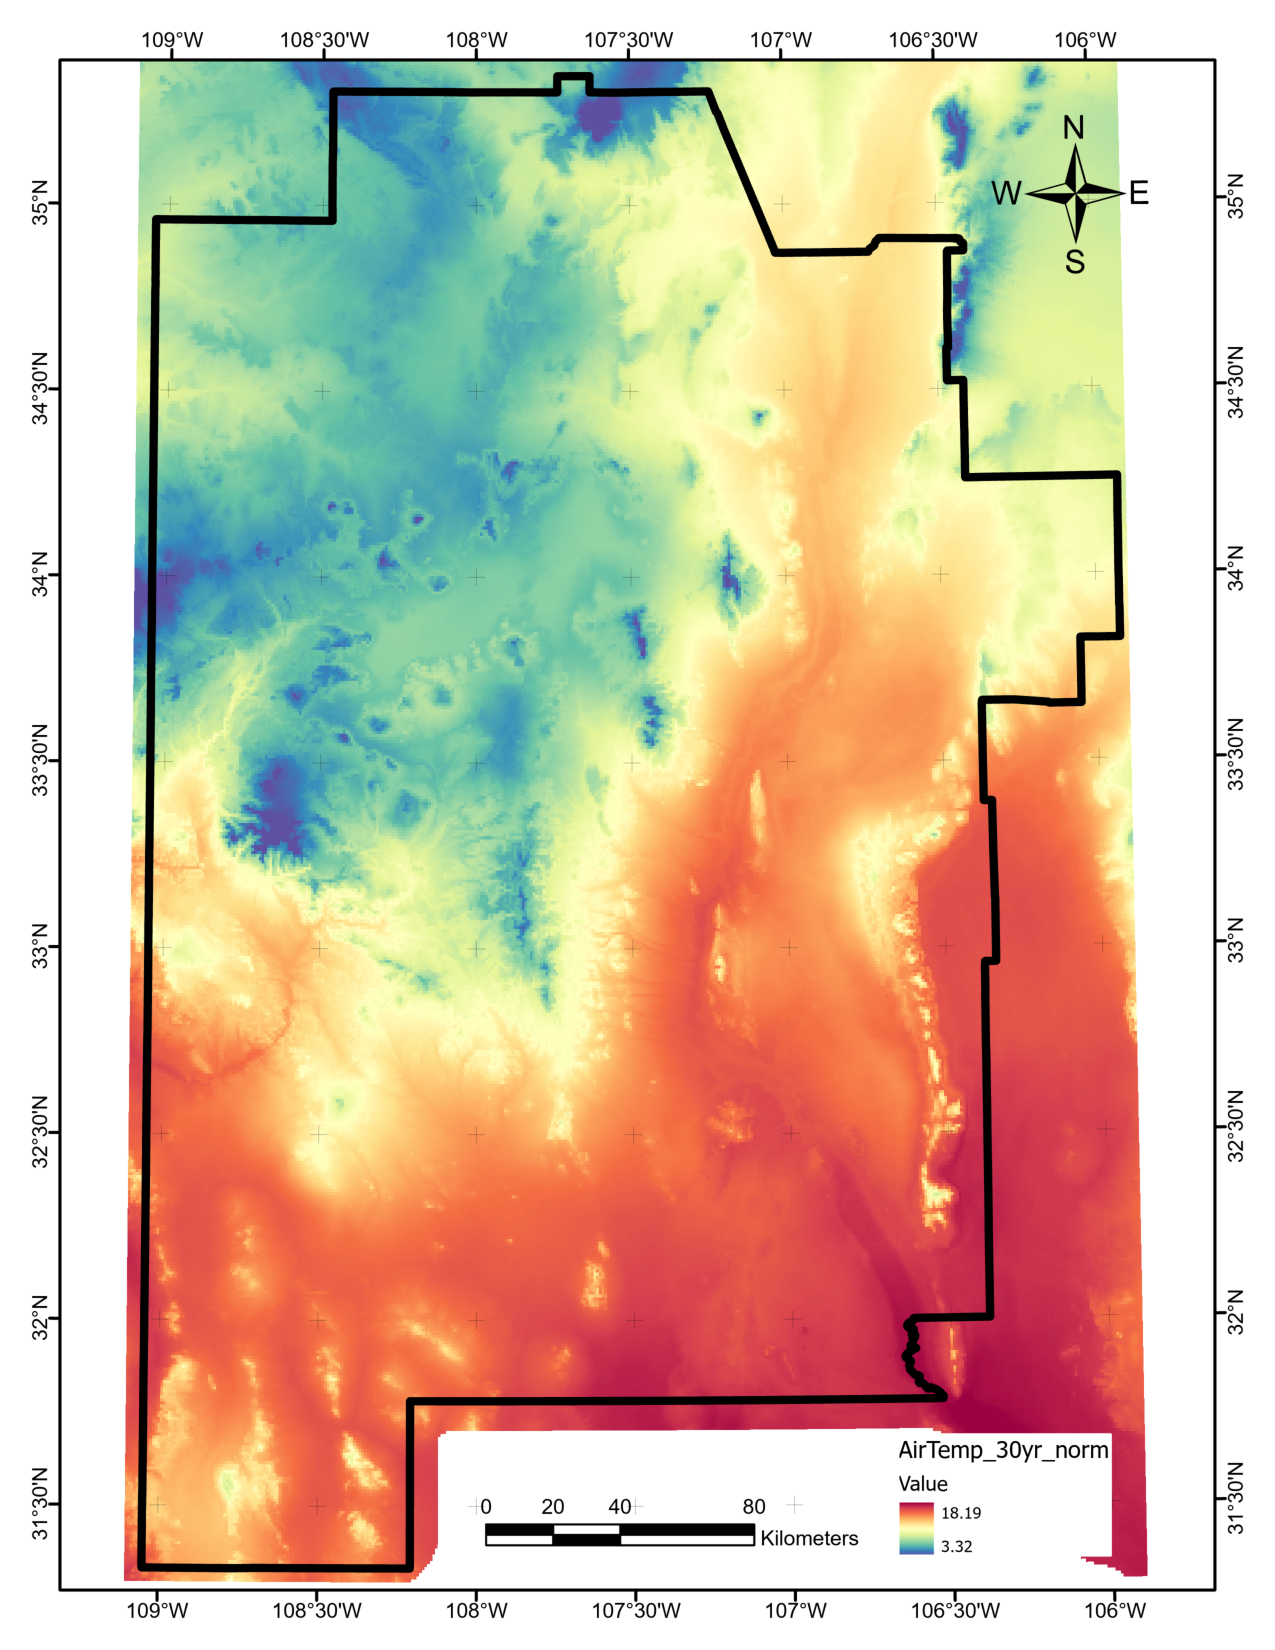
\includegraphics[scale=.50]{Figure-AvgAirTemp}
\caption[Average air temperature data layer]{Average air temperature data layer. Units are in degrees Celsius. Data retrieved from \protect\citep{prism_prism_2021}.}
\label{fig:feat_airtemp}
\end{figure}

\subsubsection{Average Precipitation}

The University of Oregon PRISM Climate Group also compiles 30-year normals for average precipitation \citep{daly_physiographically_2008, prism_prism_2021}. The 800 m resolution precipitation grid was downloaded and imported into ArcGIS, then cropped to the Extent Polygon boundaries (Figure \ref{fig:feat_precip}). The layer required no further processing.

\begin{figure}[!htp]
\centering
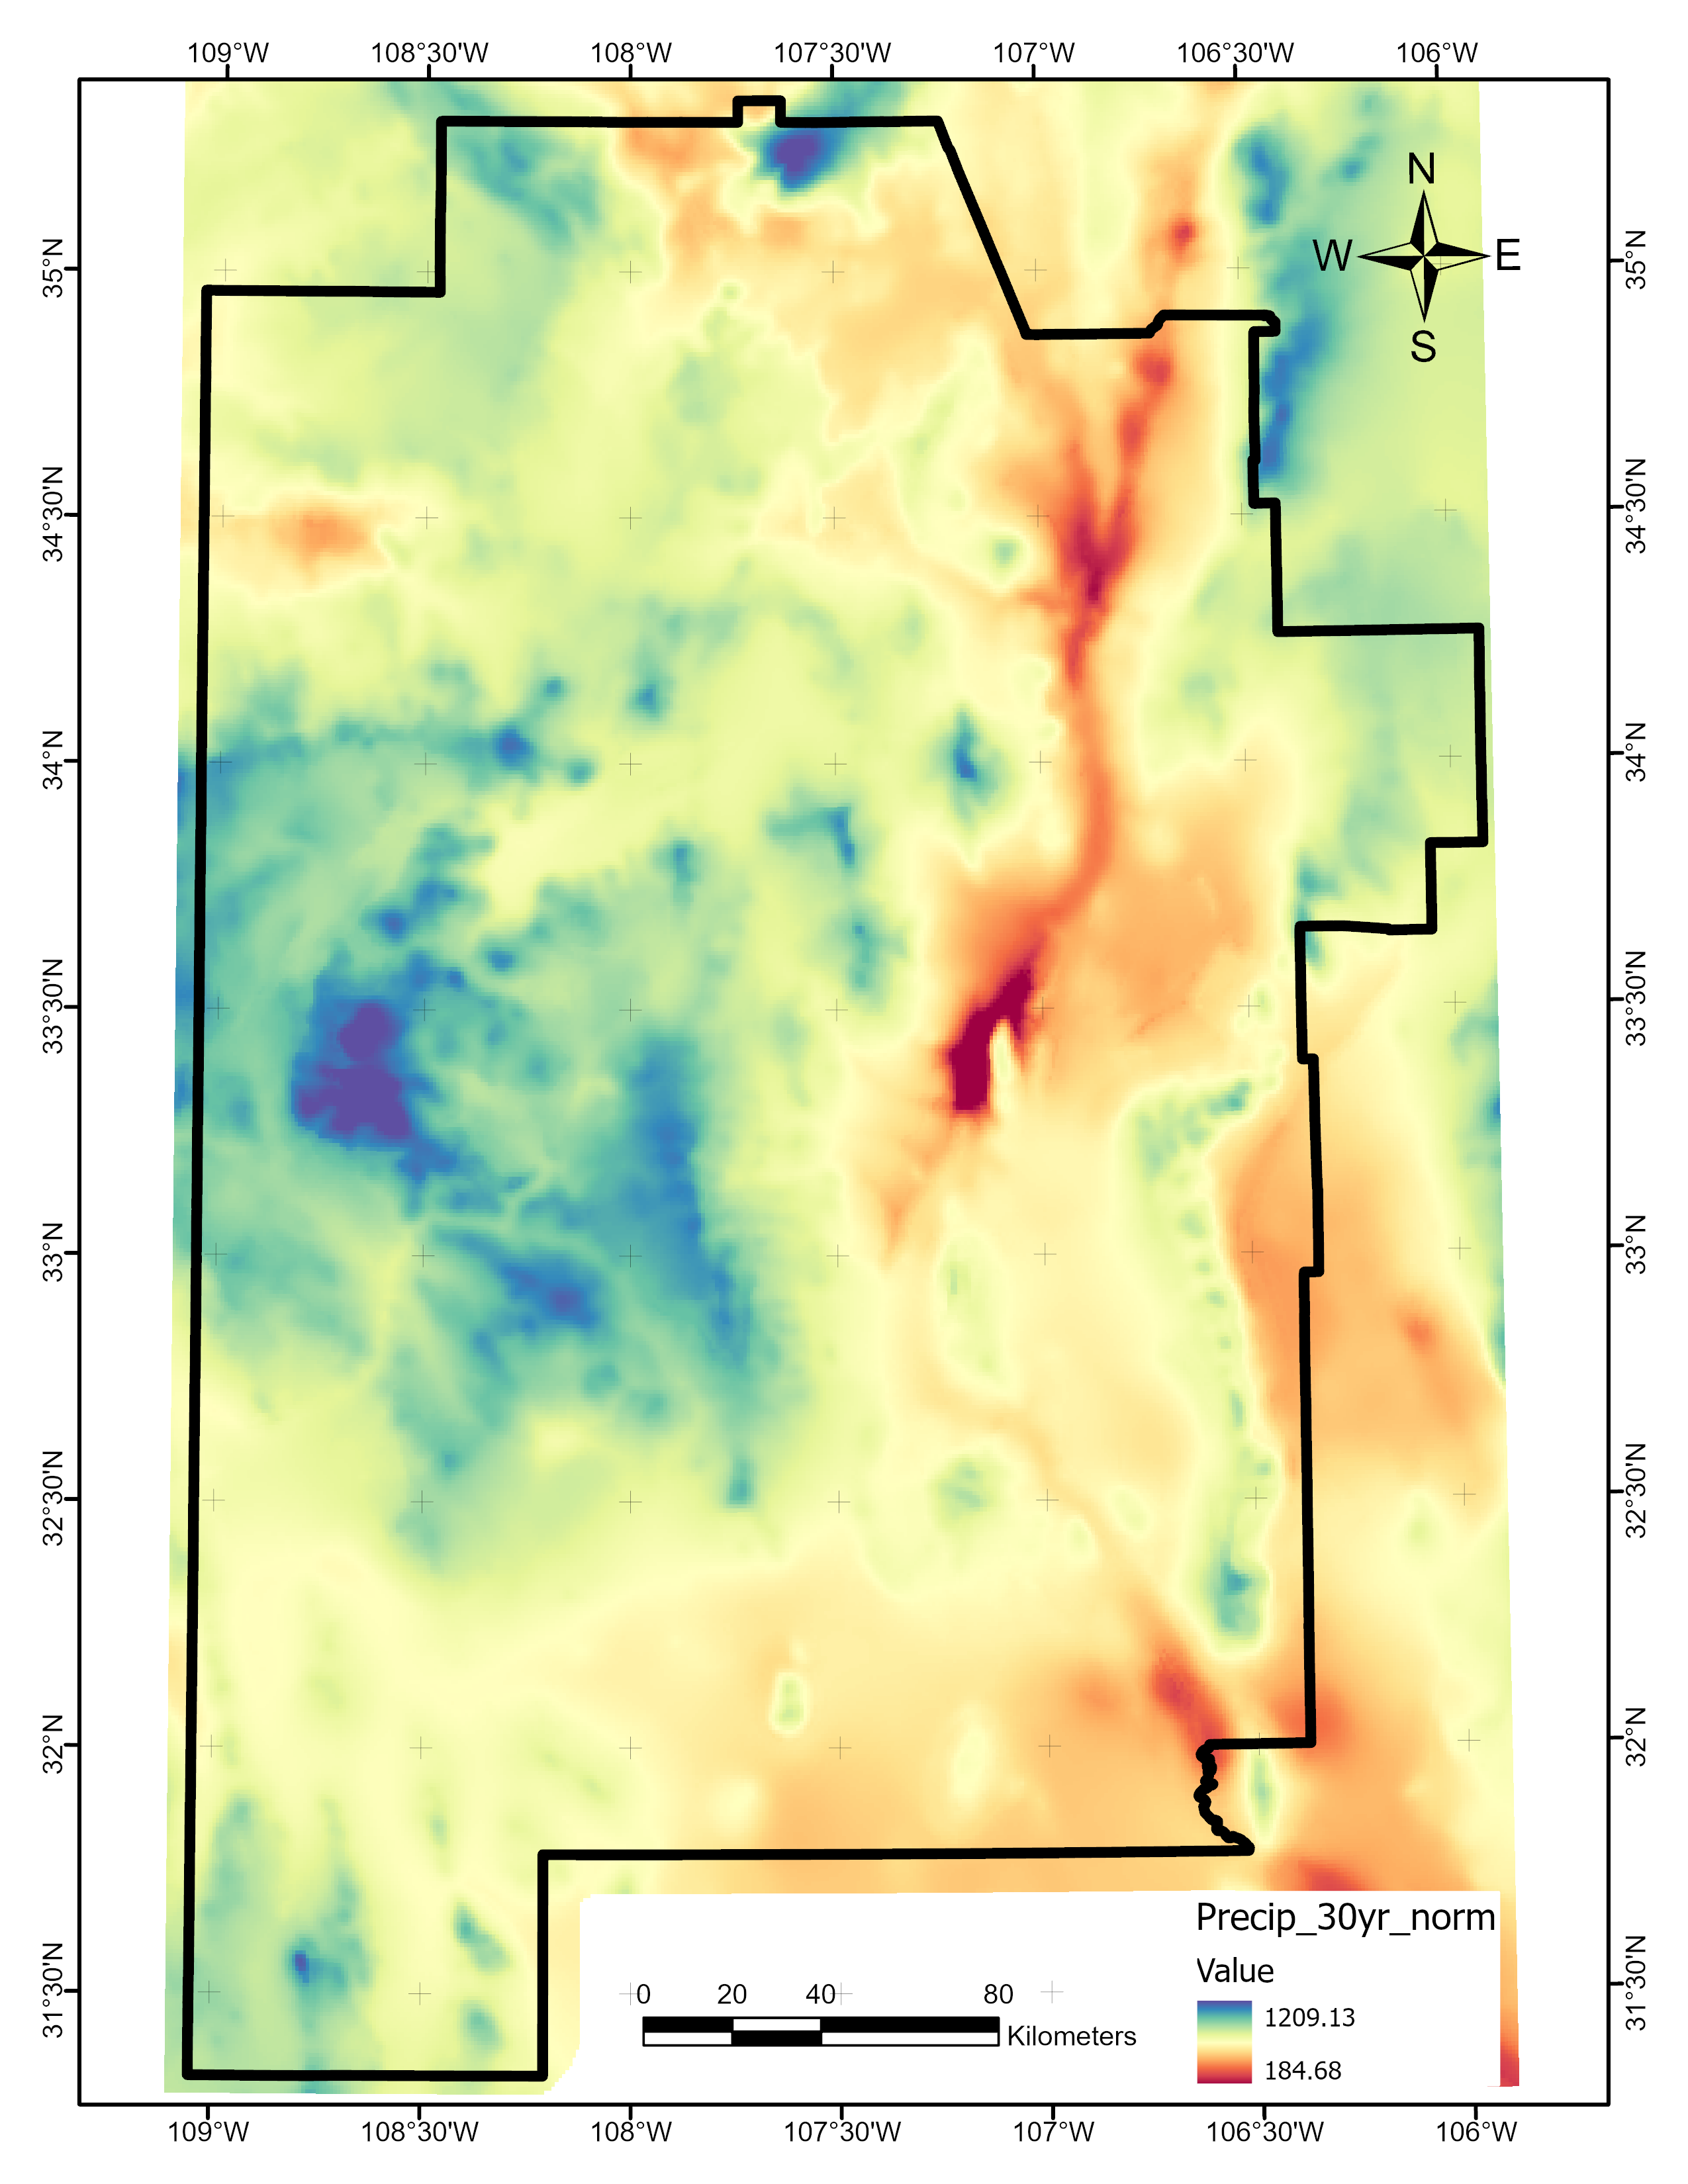
\includegraphics[scale=.50]{Figure-AvgPrecip}
\caption[Average precipitation data layer]{Average precipitation data layer in 800 m resolution. Units are in millimeters. Data retrieved from \protect\citep{prism_prism_2021}.}
\label{fig:feat_precip}
\end{figure}

\subsubsection{Basement Depth}

Following the procedure of \citeauthor{pepin_new_2018} (\citeyear{pepin_new_2018}), the basement elevation raster generated by \citeauthor{bielicki_hydrogeolgic_2015} (\citeyear{bielicki_hydrogeolgic_2015}) was downloaded, imported into ArcGIS, and processed to calculate depths. Specifically, a unit conversion from feet to meters was applied. Then, values were extracted on the point fishnet (see \ref{ssn:fishnet}), which highlighted missing data patches in the data. The ArcGIS \textit{Kriging} function interpolated values across these patches using the Ordinary method with Spherical semivariogram, a lag size of 0.096969 automatically determined by ArcGIS, and a variable search radius with a 4-point requirement. Basement depths were then calculated by subtracting the interpolated elevation layer from the surface topography (DEM) layer. However, the higher resolution of the DEM layer caused an imprint of detailed surface geomorphologies to appear on the calculated basement depth layer. To correct for this, the DEM layer was low pass filtered using the ArcGIS \textit{Filter} method, which averages a 3x3 neighborhood around each point in the data set. The final basement elevation layer (Figugre \ref{fig:feat_basementdepth}) was generated from the difference between the low-pass filtered DEM and the kriged basement depth.

\begin{figure}[h!]
\centering
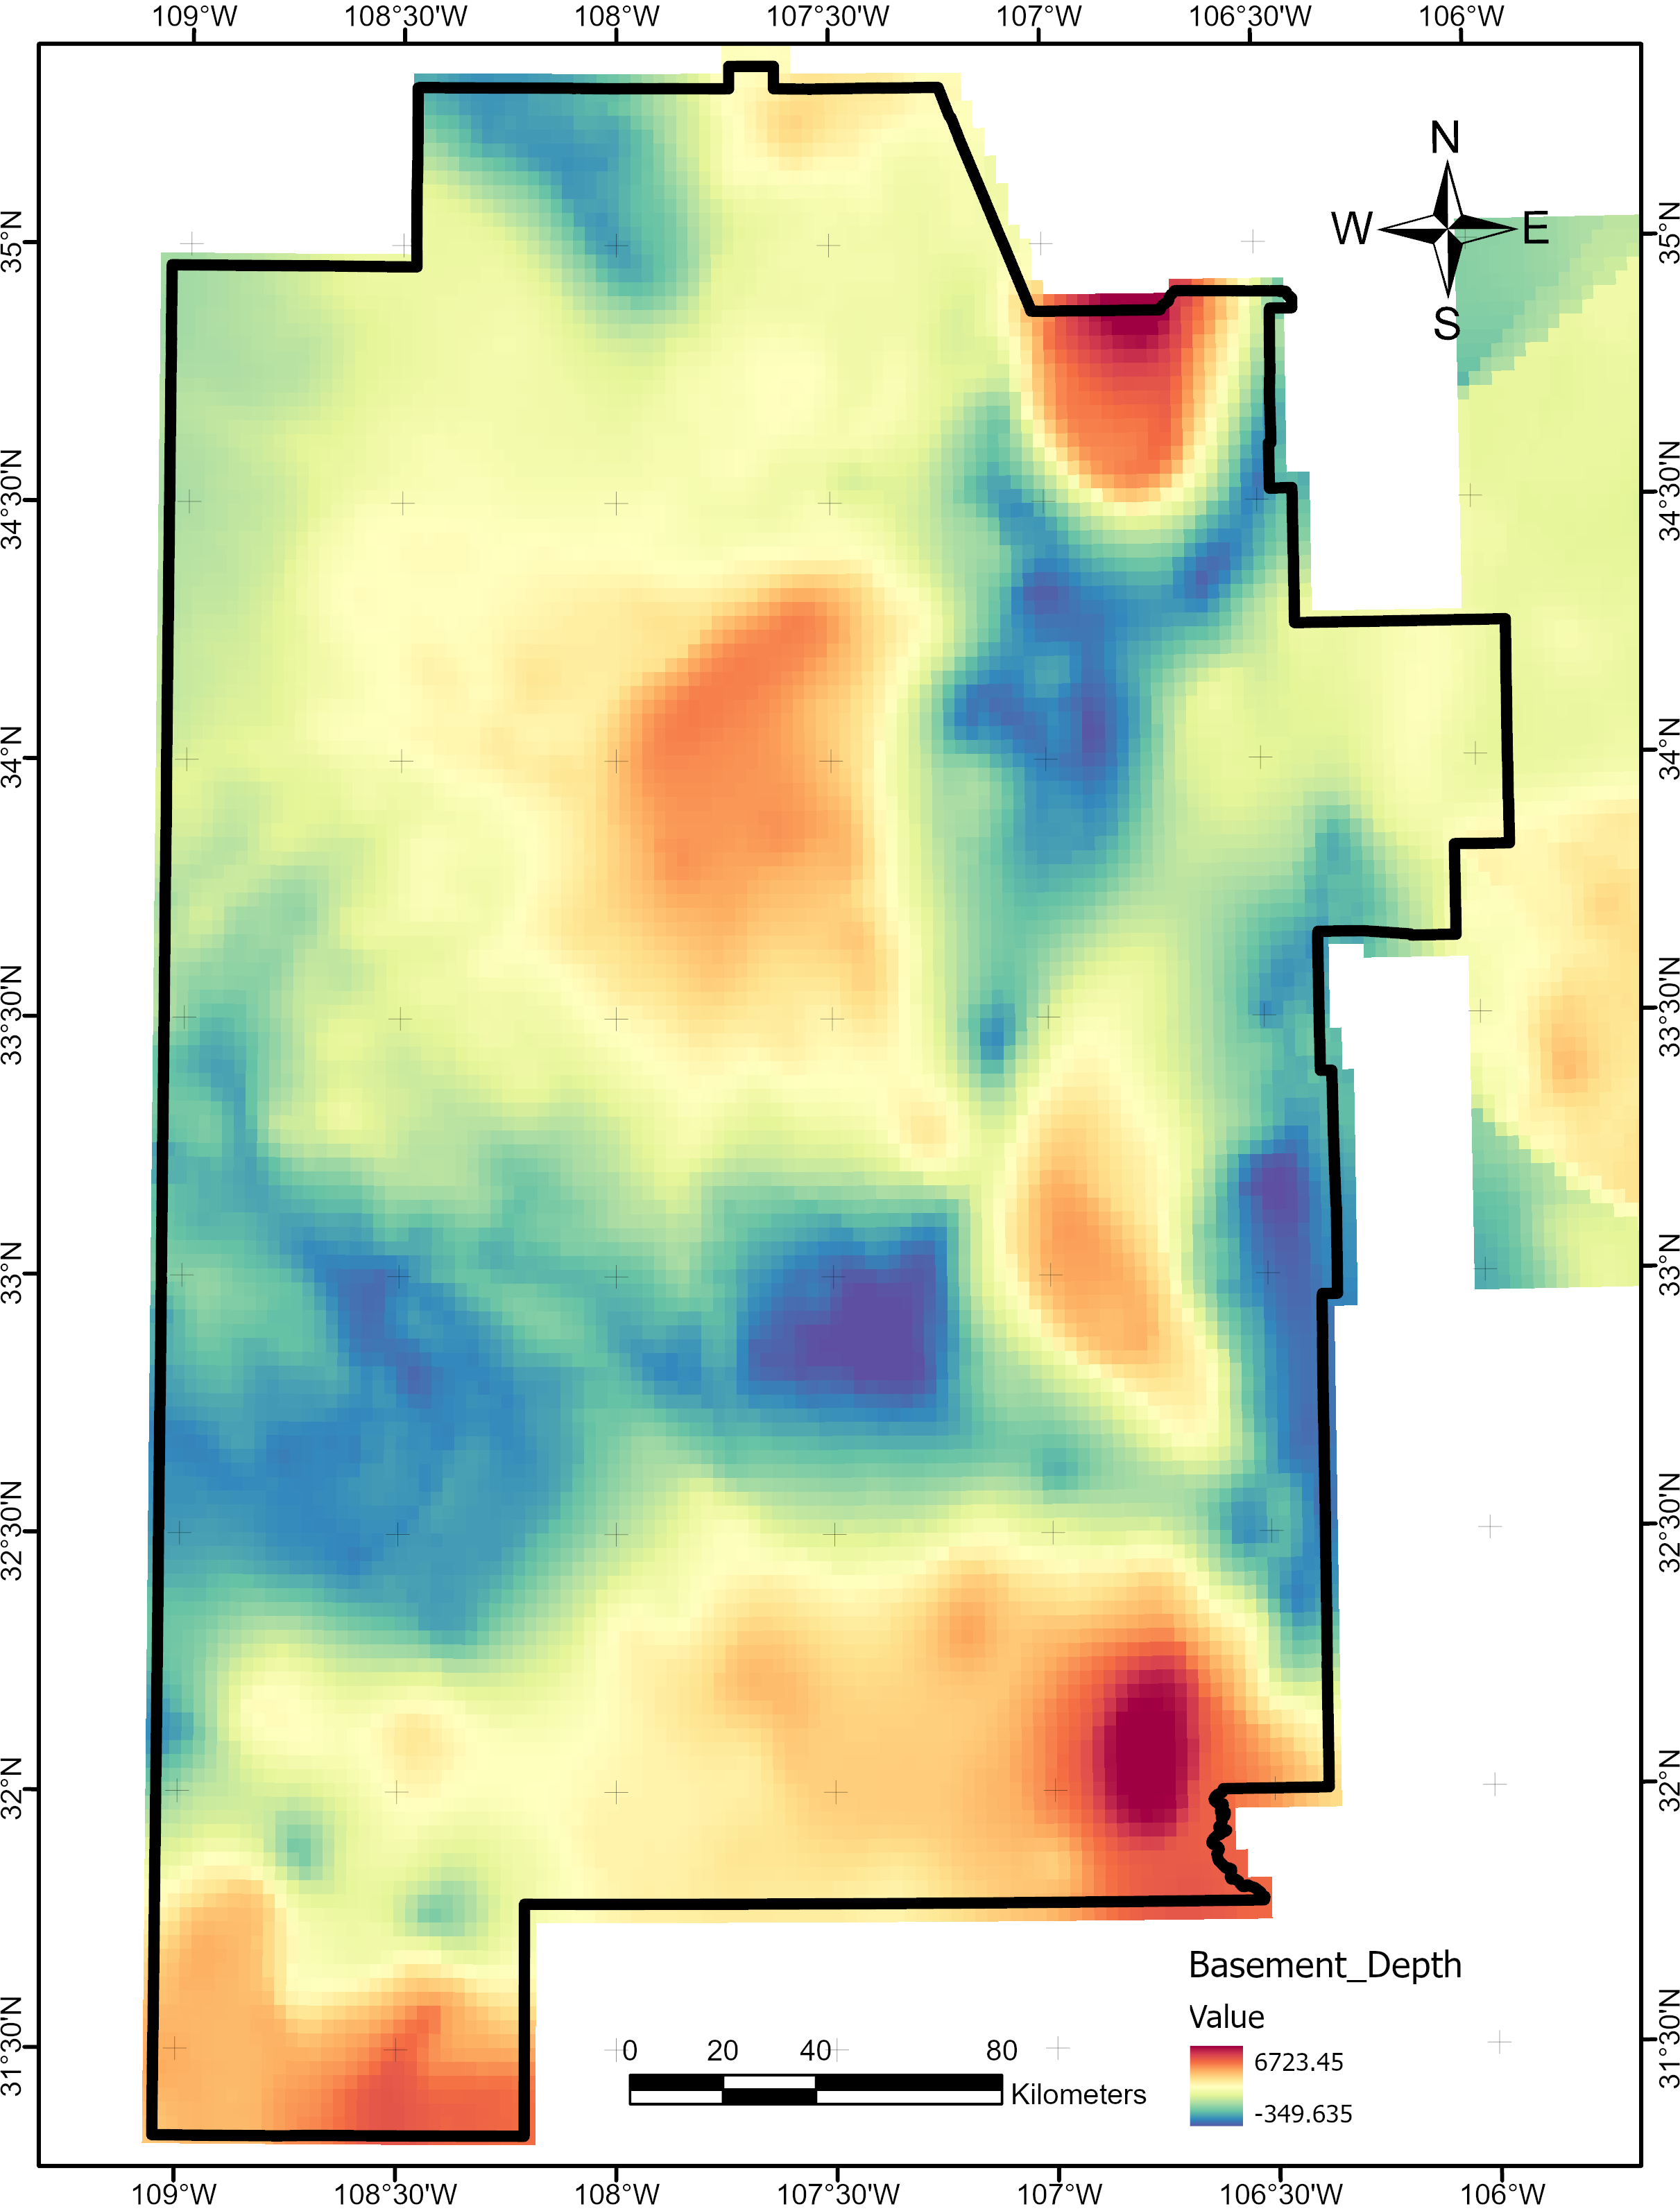
\includegraphics[scale=.50]{Figure-BasementDepth}
\caption[Basement depth data layer]{Basement depth data layer. Units are in meters. Layer based on basement elevation raster from \protect\citep{bielicki_hydrogeolgic_2015}.}
\label{fig:feat_basementdepth}
\end{figure}

\subsubsection{Boron Concentration}

Measurements of boron concentration were originally assembled by \citeauthor{bielicki_hydrogeolgic_2015} (\citeyear{bielicki_hydrogeolgic_2015}) from multiple sources ranging from USGS records to student dissertations. These data were downloaded from the OpenEI submission \citep{kelley_geothermal_2015} and merged together using ArcGIS and Python to create a single dataframe of 5686 measurements, all within the broader Extent Polygon bounds to avoid surface creation edge effects within the tighter AOI. The inconsistent spatial distribution of the data and sometimes significant variation among overlapping values from different measurement years created a unique challenge for making a representative GIS layer to use for analysis. An initial attempt to fit and interpolate the data using tuned Gaussian Process models created feature layers with too much local structure and little character away from the input data points. The ArcGIS \textit{Empirical Bayes Kriging} routine was selected instead due to its unique characteristics. For the final layer, EBK was applied with the Empirical data transformation type, a maximum of 100 points in each local model, 100 simulated semivariograms with K-Bessel model type, and a standard circular search neighborhood with a radius of 1.1957 (auto-generated), minimum of 10 neighbors, and maximum of 15 neighbors. The output grid cell size was set to 0.01 degrees. Of important note: the calculation option to include all coincident data was selected, so all overlapping measurements were considered in generating the final layer (Figure \ref{fig:feat_boron}).

\begin{figure}[!htp]
\centering
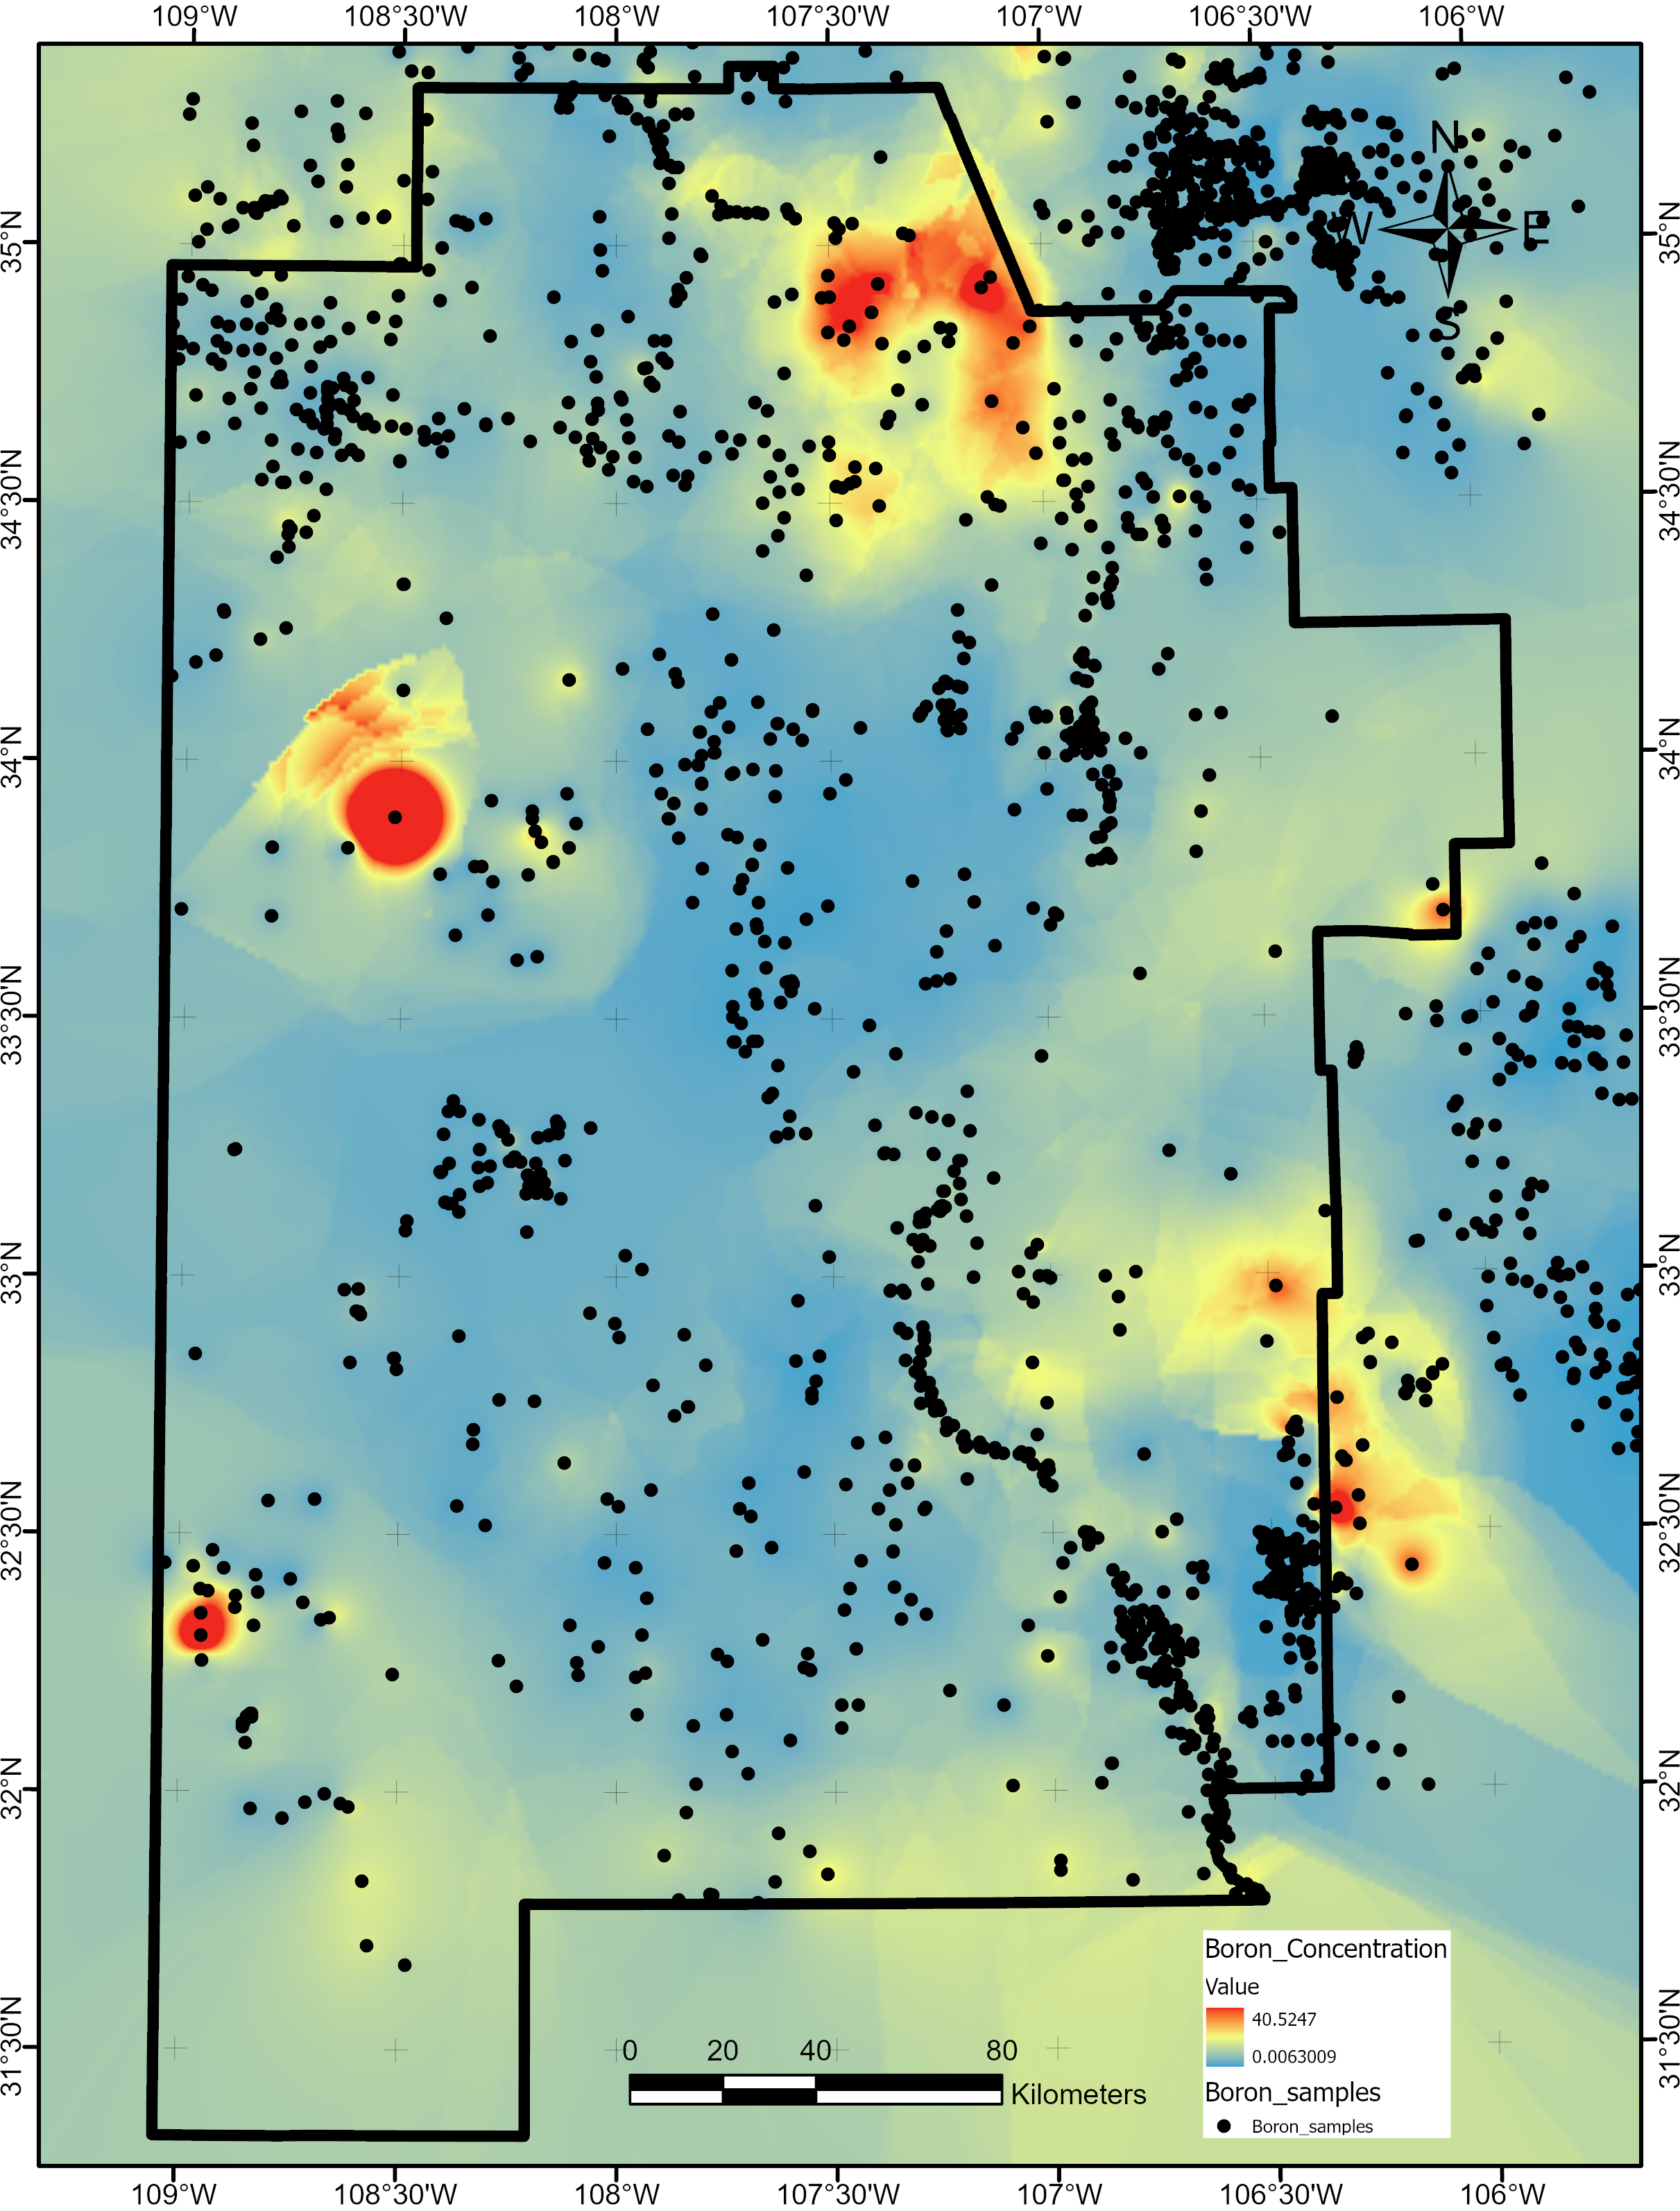
\includegraphics[scale=.50]{Figure-Boron}
\caption[Boron concentration data layer]{Boron concentration data layer. Units are in ppm or mg/L. Black dots indicate sample locations in complete data set from \protect\citep{bielicki_hydrogeolgic_2015}.}
\label{fig:feat_boron}
\end{figure}

\subsubsection{Crustal Thickness}

In the absence of a more recent seismic study constraining variations in crustal thickness across the study area, the 2.5D regional map published by \citeauthor{keller_comparative_1991} (\citeyear{keller_comparative_1991}) was to construct the crustal thickness feature layer. Similar to the procedure described in \citep{pepin_new_2018}, the Keller map was georeferenced in ArcGIS, and thickness contours were manually digitized as polylines. These polylines continued slightly beyond the AOI boundary to ensure proper constraints for surface creation without artifacts near the AOI edges. The ArcGIS function \textit{Feature to 3D by Attribute} converted the polylines into 3D contours, and \textit{Topo to Raster} interpolated the contours into a continuous final grid (Figure \ref{fig:feat_crust}). Since the Keller map was derived from low-resolution seismic lines from the 1960s-1980s, the result is a very low frequency approximation for crustal thickness variations associated with the CP and RGR. As such, \textit{Topo to Raster} a larger cell size of 0.025 degrees was used. Other parameters choices include: margin in the cells of 20, smallest z value for interpolation of 25, largest z value for the interpolation of 55, Enforce selection for drainage enforcement, and maximum iterations of 20.

\begin{figure}[!htp]
\centering
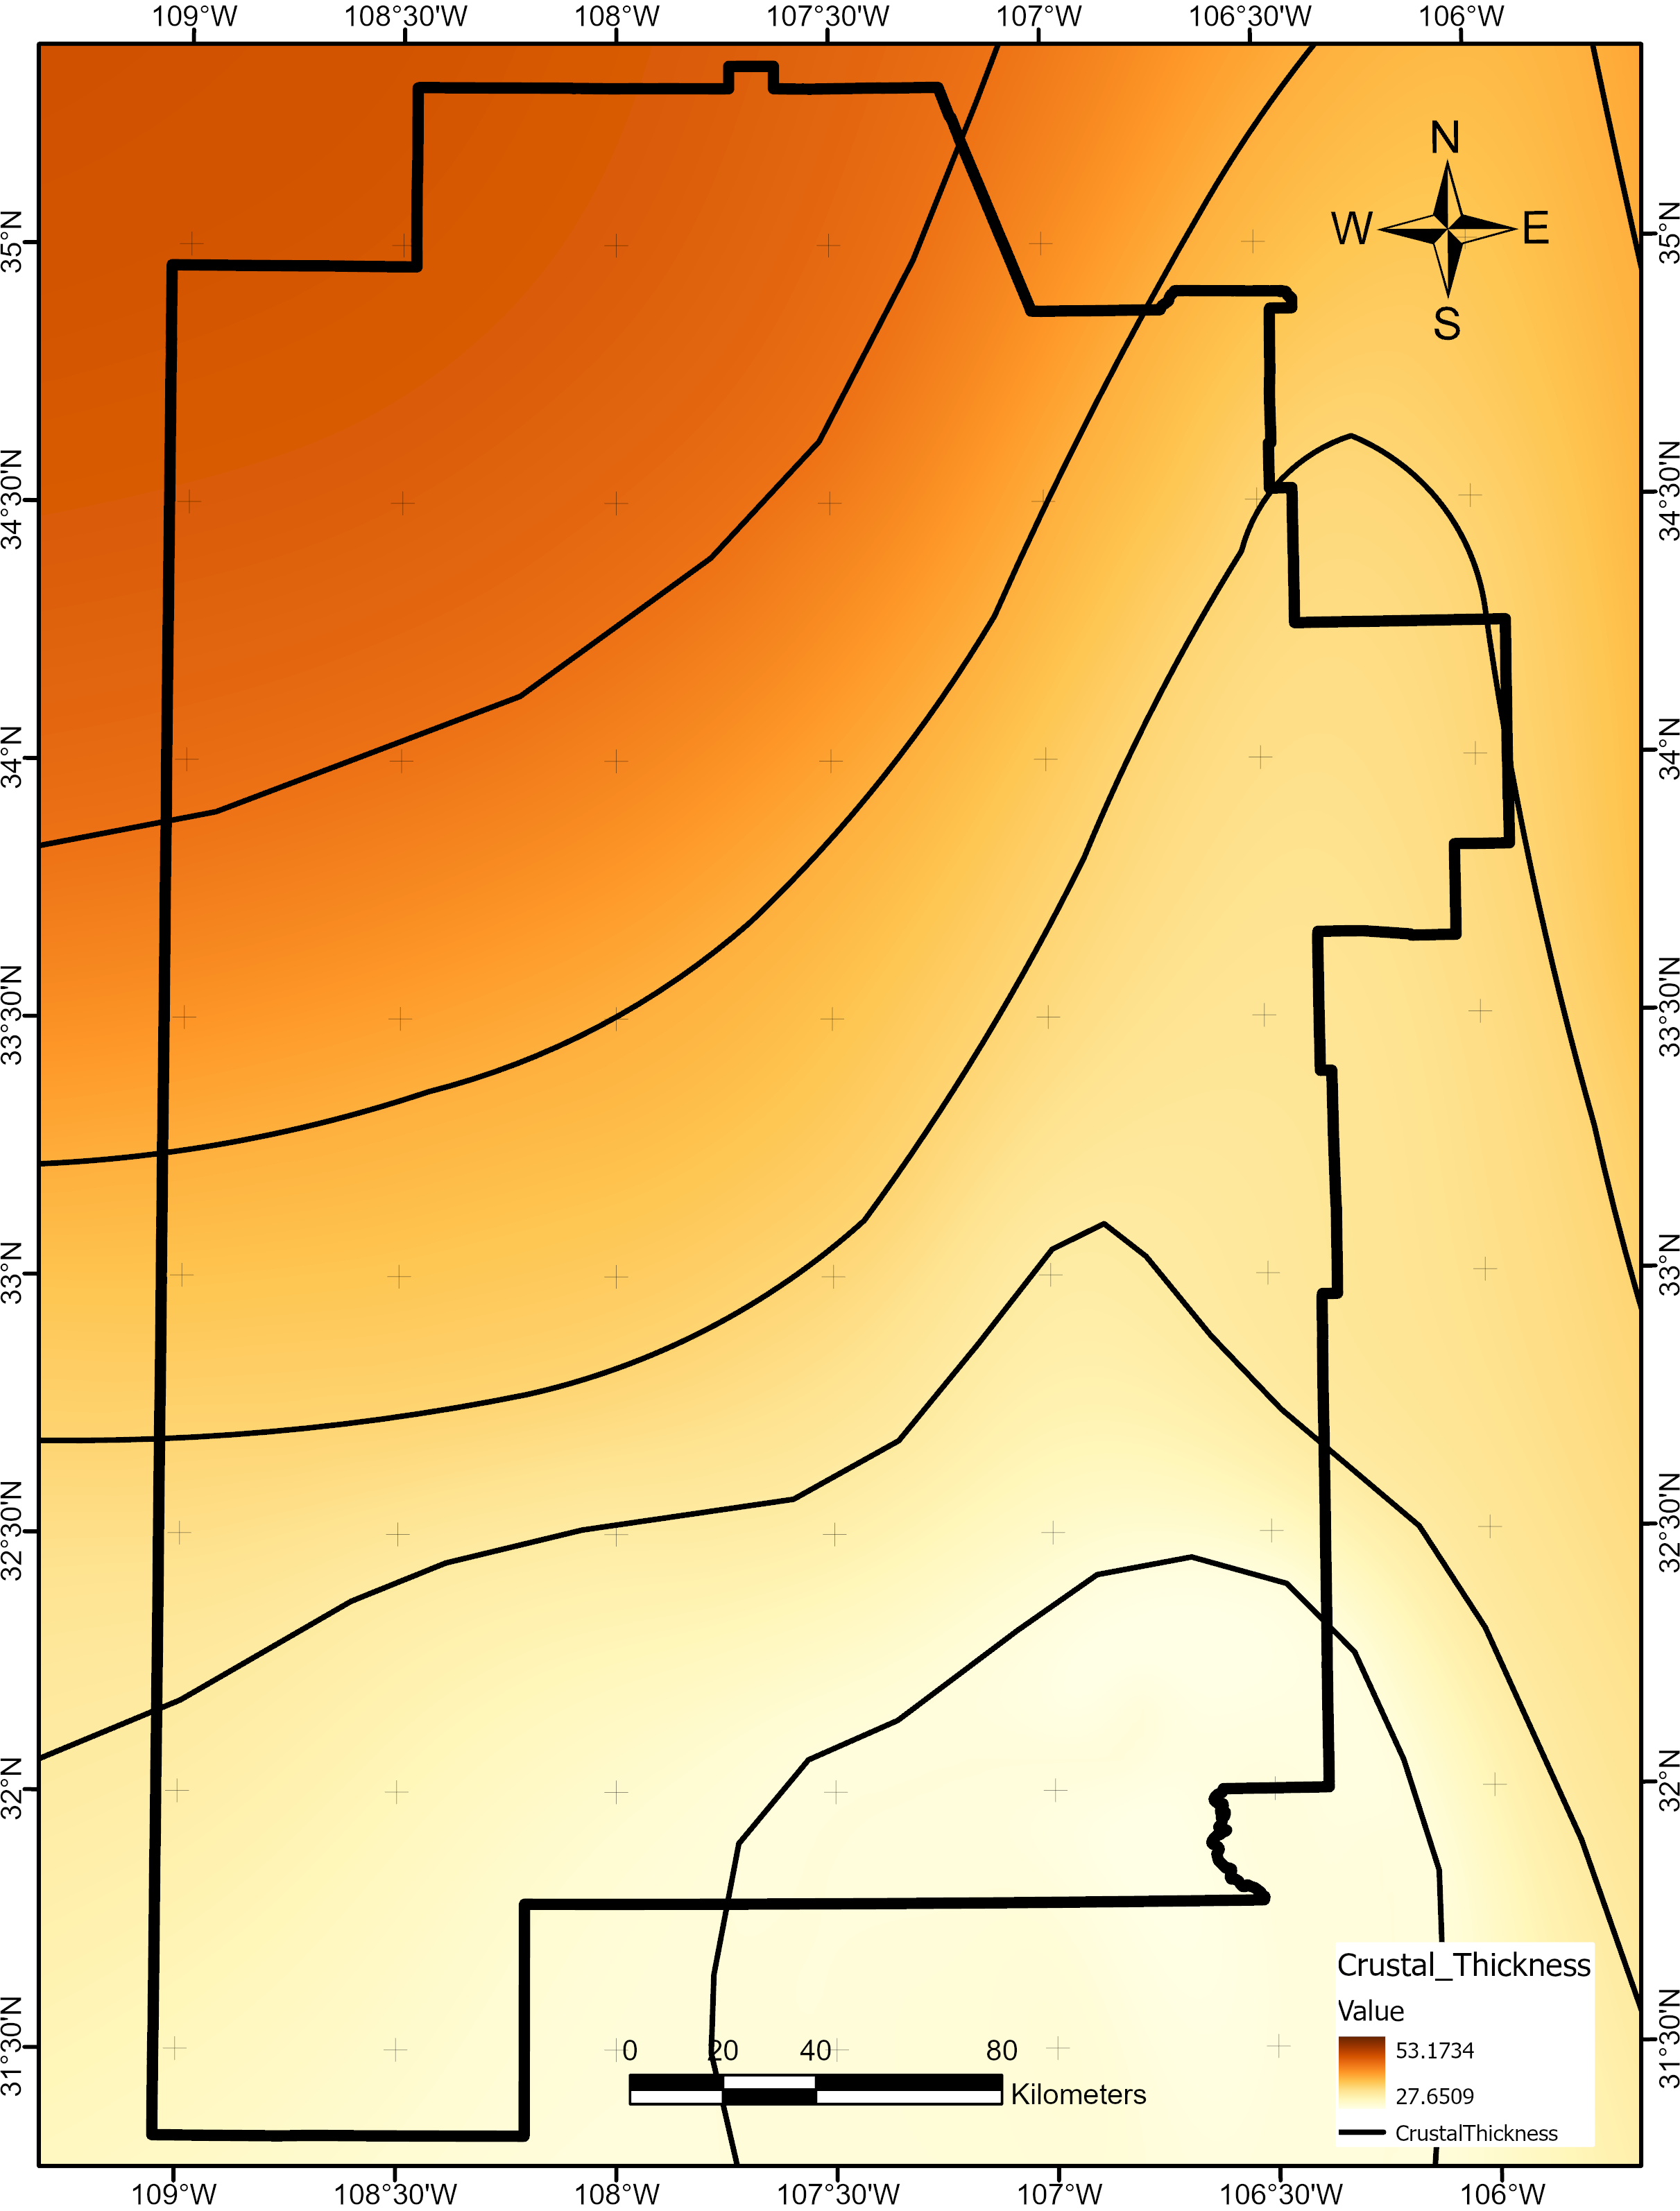
\includegraphics[scale=.50]{Figure-CrustalThickness}
\caption[Crustal thickness data layer]{Crustal thickness data layer. Units are in kilometers. Black lines refer to contours digitized from \protect\citep{keller_comparative_1991}.}
\label{fig:feat_crust}
\end{figure}

\subsubsection{Drainage Density}

Drainage polyline data comes from the \citep{bielicki_hydrogeolgic_2015} PFA OpenEI submission \citep{kelley_geothermal_2015}. The data were downloaded and imported into ArcGIS, then compared to the DEM later for quality control. A couple of methods were attempted in order to transform this feature into a continuous-valued layer with full map coverage. First, the polylines were converted to points with 500 m sampling. This point set was loaded into a Python script, which used a grid search routine to determine the best radius for a Gaussian kernel density operator. Ten-fold cross validation was employed, which splits the data into 10 subsets and interchangeably trains on 9, tests on one to get an average performance score. Based on a calculation of the negative log likelihood, the best radius was found to be 45,600 m. However, when the kernel density operation is applied to the data with this radius, the map shows a central blob of high density, which falls off toward the sides of the survey. With such a high radius, edge effects come into play since no drainage polylines were available outside of the AOI boundary. Furthermore, the conversion of line data to points for this method disregards the spatial relationships of the connected line data. The ArcGIS version of kernel density uses an adapted quartic kernel function described by \citep{silverman_density_2018} to fit a smoothly-curved surface over polylines with a maximum value over the line and sides that taper to zero based on the search radius. Default search radius values come from a bandwidth calculation, also based on Silverman book \citep{esri_how_2021,silverman_density_2018}. Densities are calculated as the cumulative sum of the overlapping curve fits for all polylines in a data set. This method operates on the polyline features directly and results in a map with much more drainage variation within the AOI. The final drainage density layer (Figure \ref{fig:feat_drainage}) was generated using this methodology with an output cell size of 0.0025 degrees and an auto-generated search radius of 0.2716.

\begin{figure}[!htp]
\centering
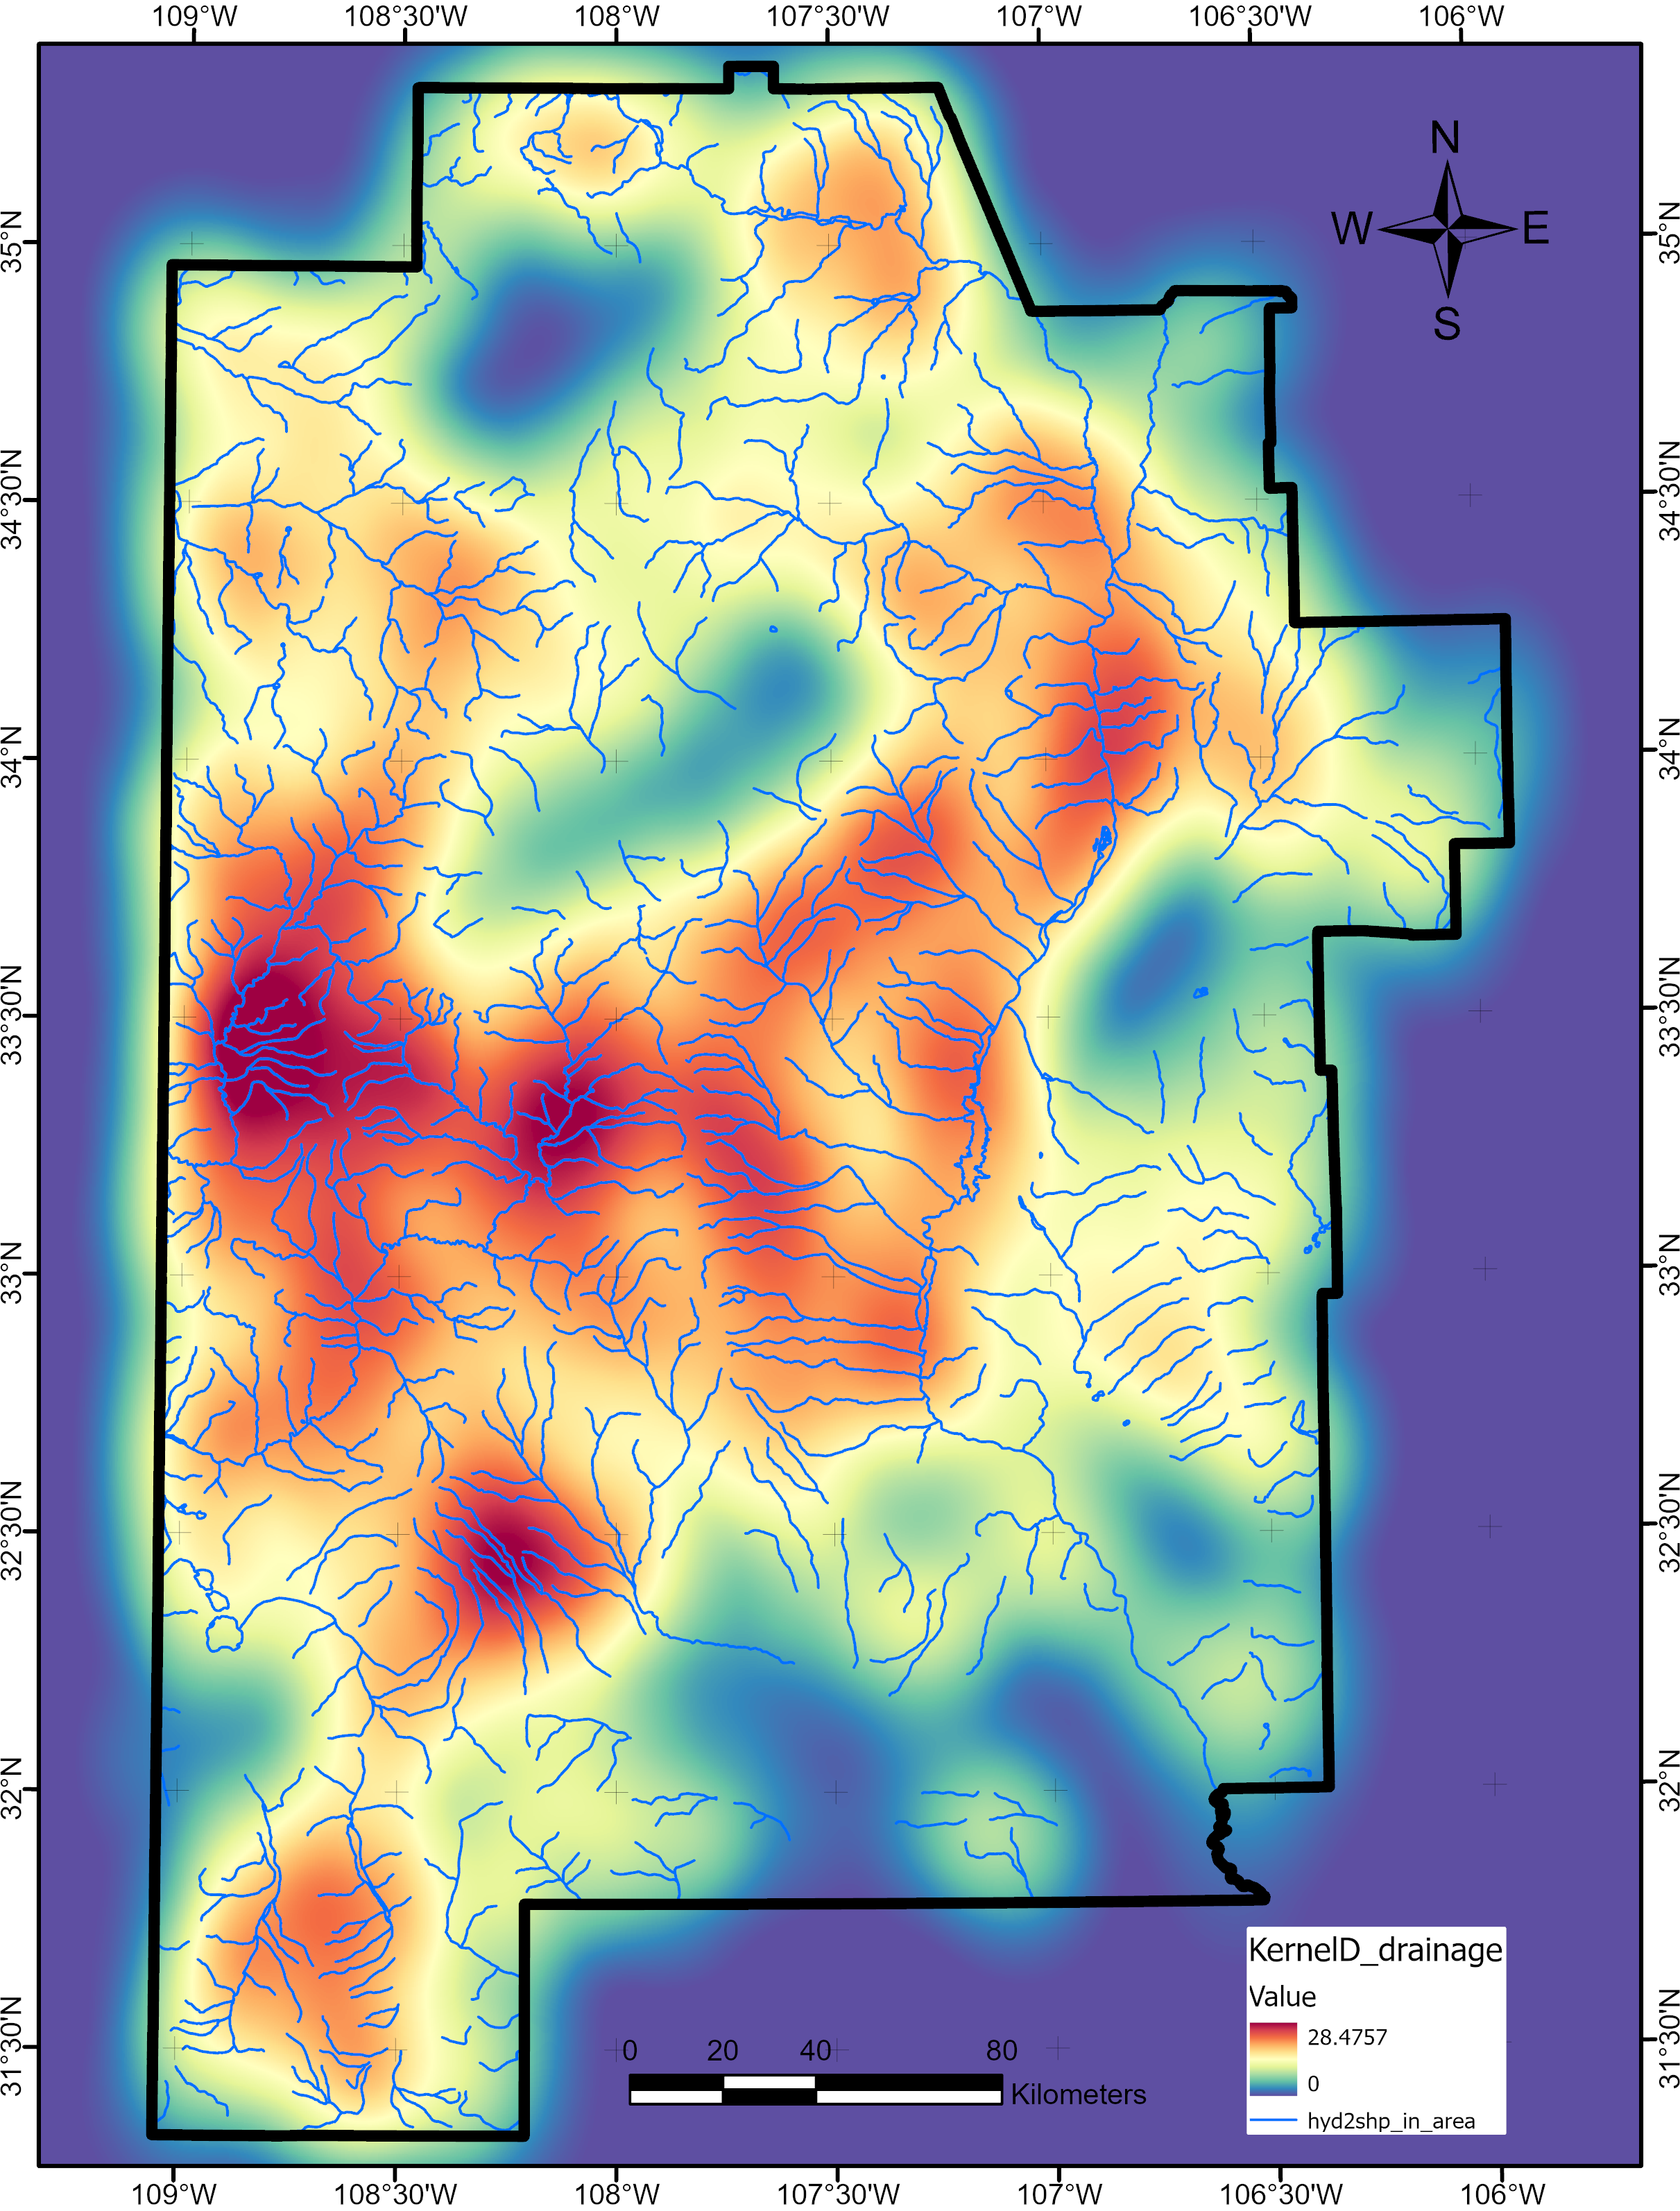
\includegraphics[scale=.50]{Figure-Drainage}
\caption[Drainage density data layer]{Drainage density data layer. Units are in degrees/square degrees. Blue lines show the drainage polyline data set from \protect\citep{bielicki_hydrogeolgic_2015}.}
\label{fig:feat_drainage}
\end{figure}

\subsubsection{Earthquake Density}

Following the procedure outlined by \citeauthor{pepin_new_2018} (\citeyear{pepin_new_2018}), an earthquake data set for southwest New Mexico was created by combining historical earthquake catalogs for 1869-1998 \citep{sanford_earthquake_2002}, 1999-2004 \citep{sanford_earthquake_2006}, and 2005-2009 \citep{pursley_earthquake_2013} with data pulled from the USGS Earthquake catalog \citep{usgs_earthquake_2021} through to January 2021. All events were combined into a single dataframe in Python, and event duplicates were removed. The final catalog, cropped to the Extent Polygon boundary, consists of 2539 events spanning 1962-2020. This point set was loaded into a KDE Python script, which used a grid search routine to determine the best radius for a Gaussian kernel density operator. Ten-fold cross validation was employed, which splits the data into 10 subsets and then interchangeably trains on 9 and tests on one to get an average performance score. The maximum negative log likelihood indicates a best radius value of 11,600 m (Figure \ref{fig:EQ_cv}). 

\begin{figure}[!htp]
\centering
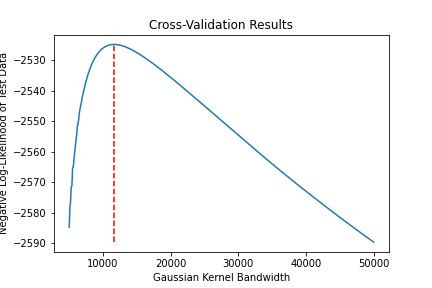
\includegraphics[scale=.50]{templates/images/Figure-Earthquake_kde_gridsearchcv_result.png}
\caption[Earthquake density parameter tuning]{Cross-validation results for earthquake KDE. Red dashed line indicates maximum negative log likelihood value identifying the best choice for kernel radius.}
\label{fig:EQ_cv}
\end{figure}

KDE values calculated at each fishnet point location were loaded into ArcGIS, and \textit{Kriging} was used to generate a final surface for plotting purposes. textit{Kriging} parameters included Ordinary kriging method, Spherical semivariogram model, lag size of 1e-6, and a variable search radius with 12-point requirement. The final earthquake density map (Figure \ref{fig:feat_EQ_density}) appears similar to Figure 3.10 in (Pepin, 2018). 

\begin{figure}[!htp]
\centering
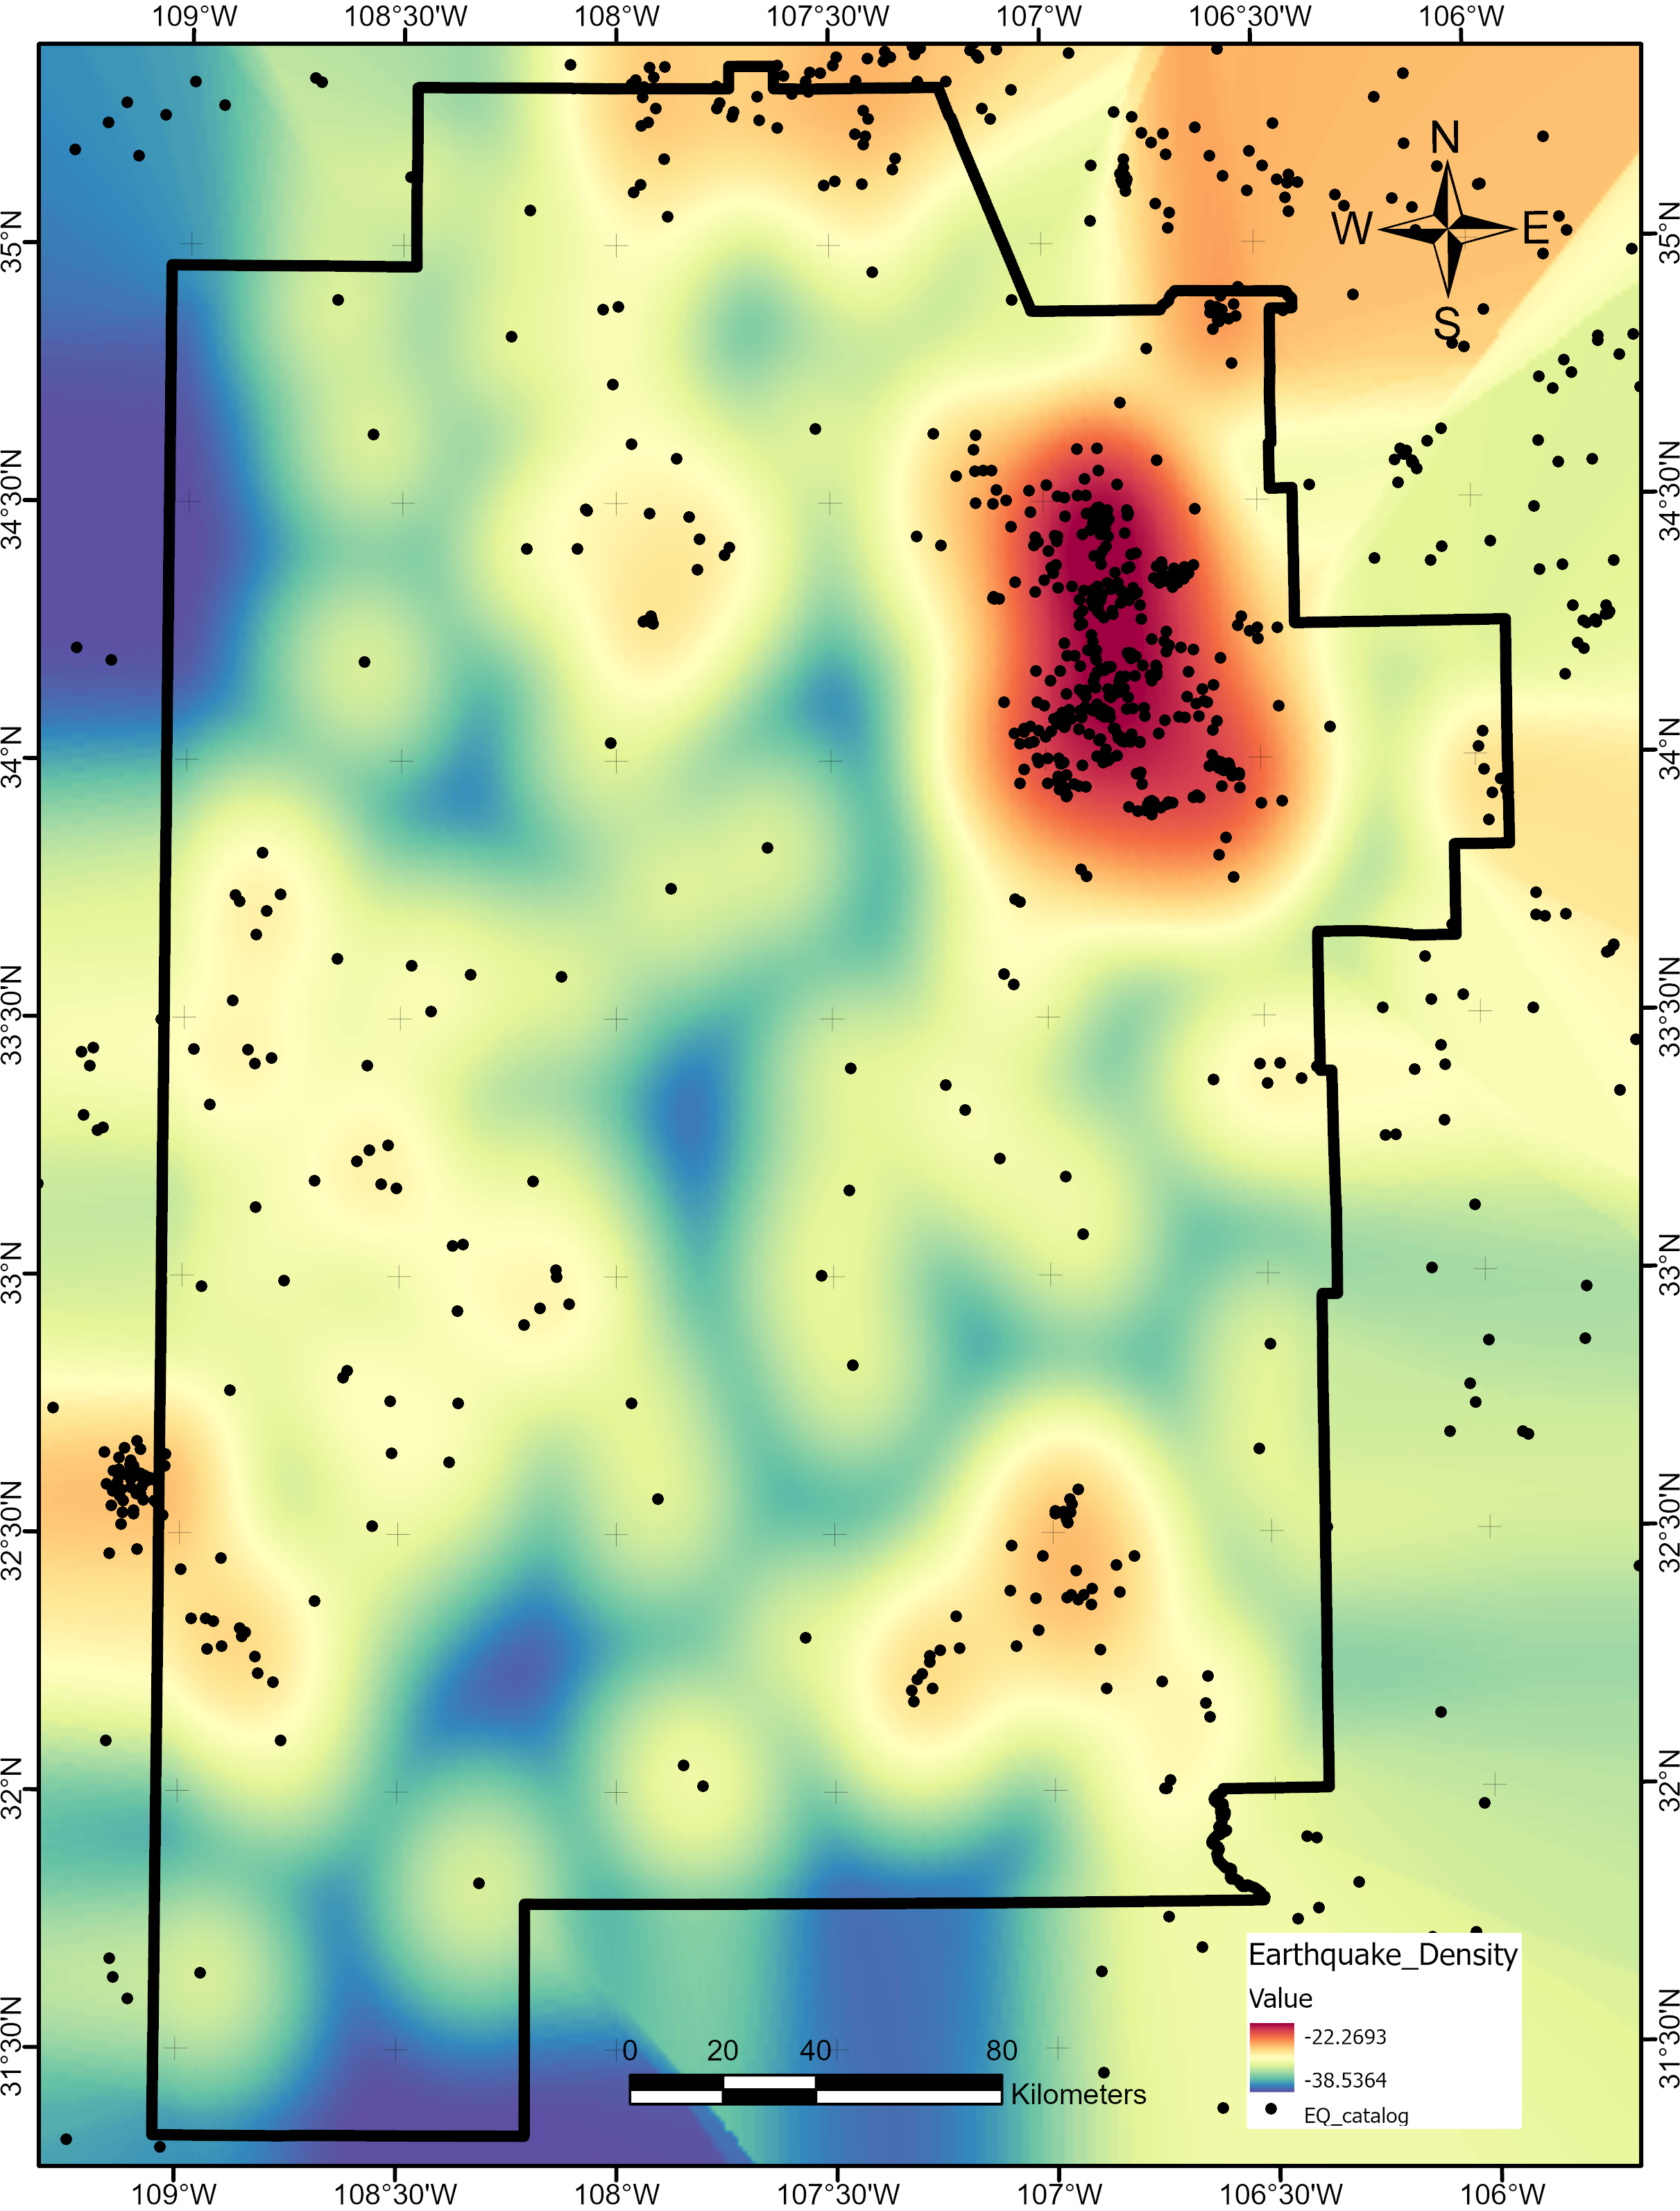
\includegraphics[scale=.50]{Figure-EarthquakeDensity}
\caption[Earthquake density data layer]{Earthquake density data layer. Units are in log density (points/\(km^2\)). Block dots indicate earthquake locations.}
\label{fig:feat_EQ_density}
\end{figure}

\subsubsection{Gamma Ray Dose Rate}

Aerial gamma-ray surveys conducted across the United States in the late 1970-1980s allowed for the construction of Potassium concentration (K, in percent K), Uranium concentration (eU, in ppm), and Thorium concentration (eTh in ppm) maps, which relate to mineralogy, lithology, and hence, stratigraphy. These measures collectively define the absorbed dose rate, which can be calculated from the following equation: \( D = 13.2 K + 5.48 eU + 2.72 eTh \) \citep{duval_terrestrial_2005}.

The absorbed dose rate for West Central USA was downloaded from the USGS Open-File Report 2005-1413 site \citep{duval_terrestrial_2005}, loaded into ArcGIS, and cropped to the Extent Polygon bounds. A data gap in the vicinity of the White Sands Missile Range to the southeast of the study area necessitated layer interpolation using kriging. Grid values were extracted using the fishnet of points, then passed through the ArcGIS \textit{Kriging} function for the final layer (Figure \ref{fig:feat_gamma}) with the following parameters: Ordinary kriging method, Spherical semivariogram model, auto-generated lag size of 0.096969, and a variable search radius with a 4-point requirement.

\begin{figure}[!htp]
\centering
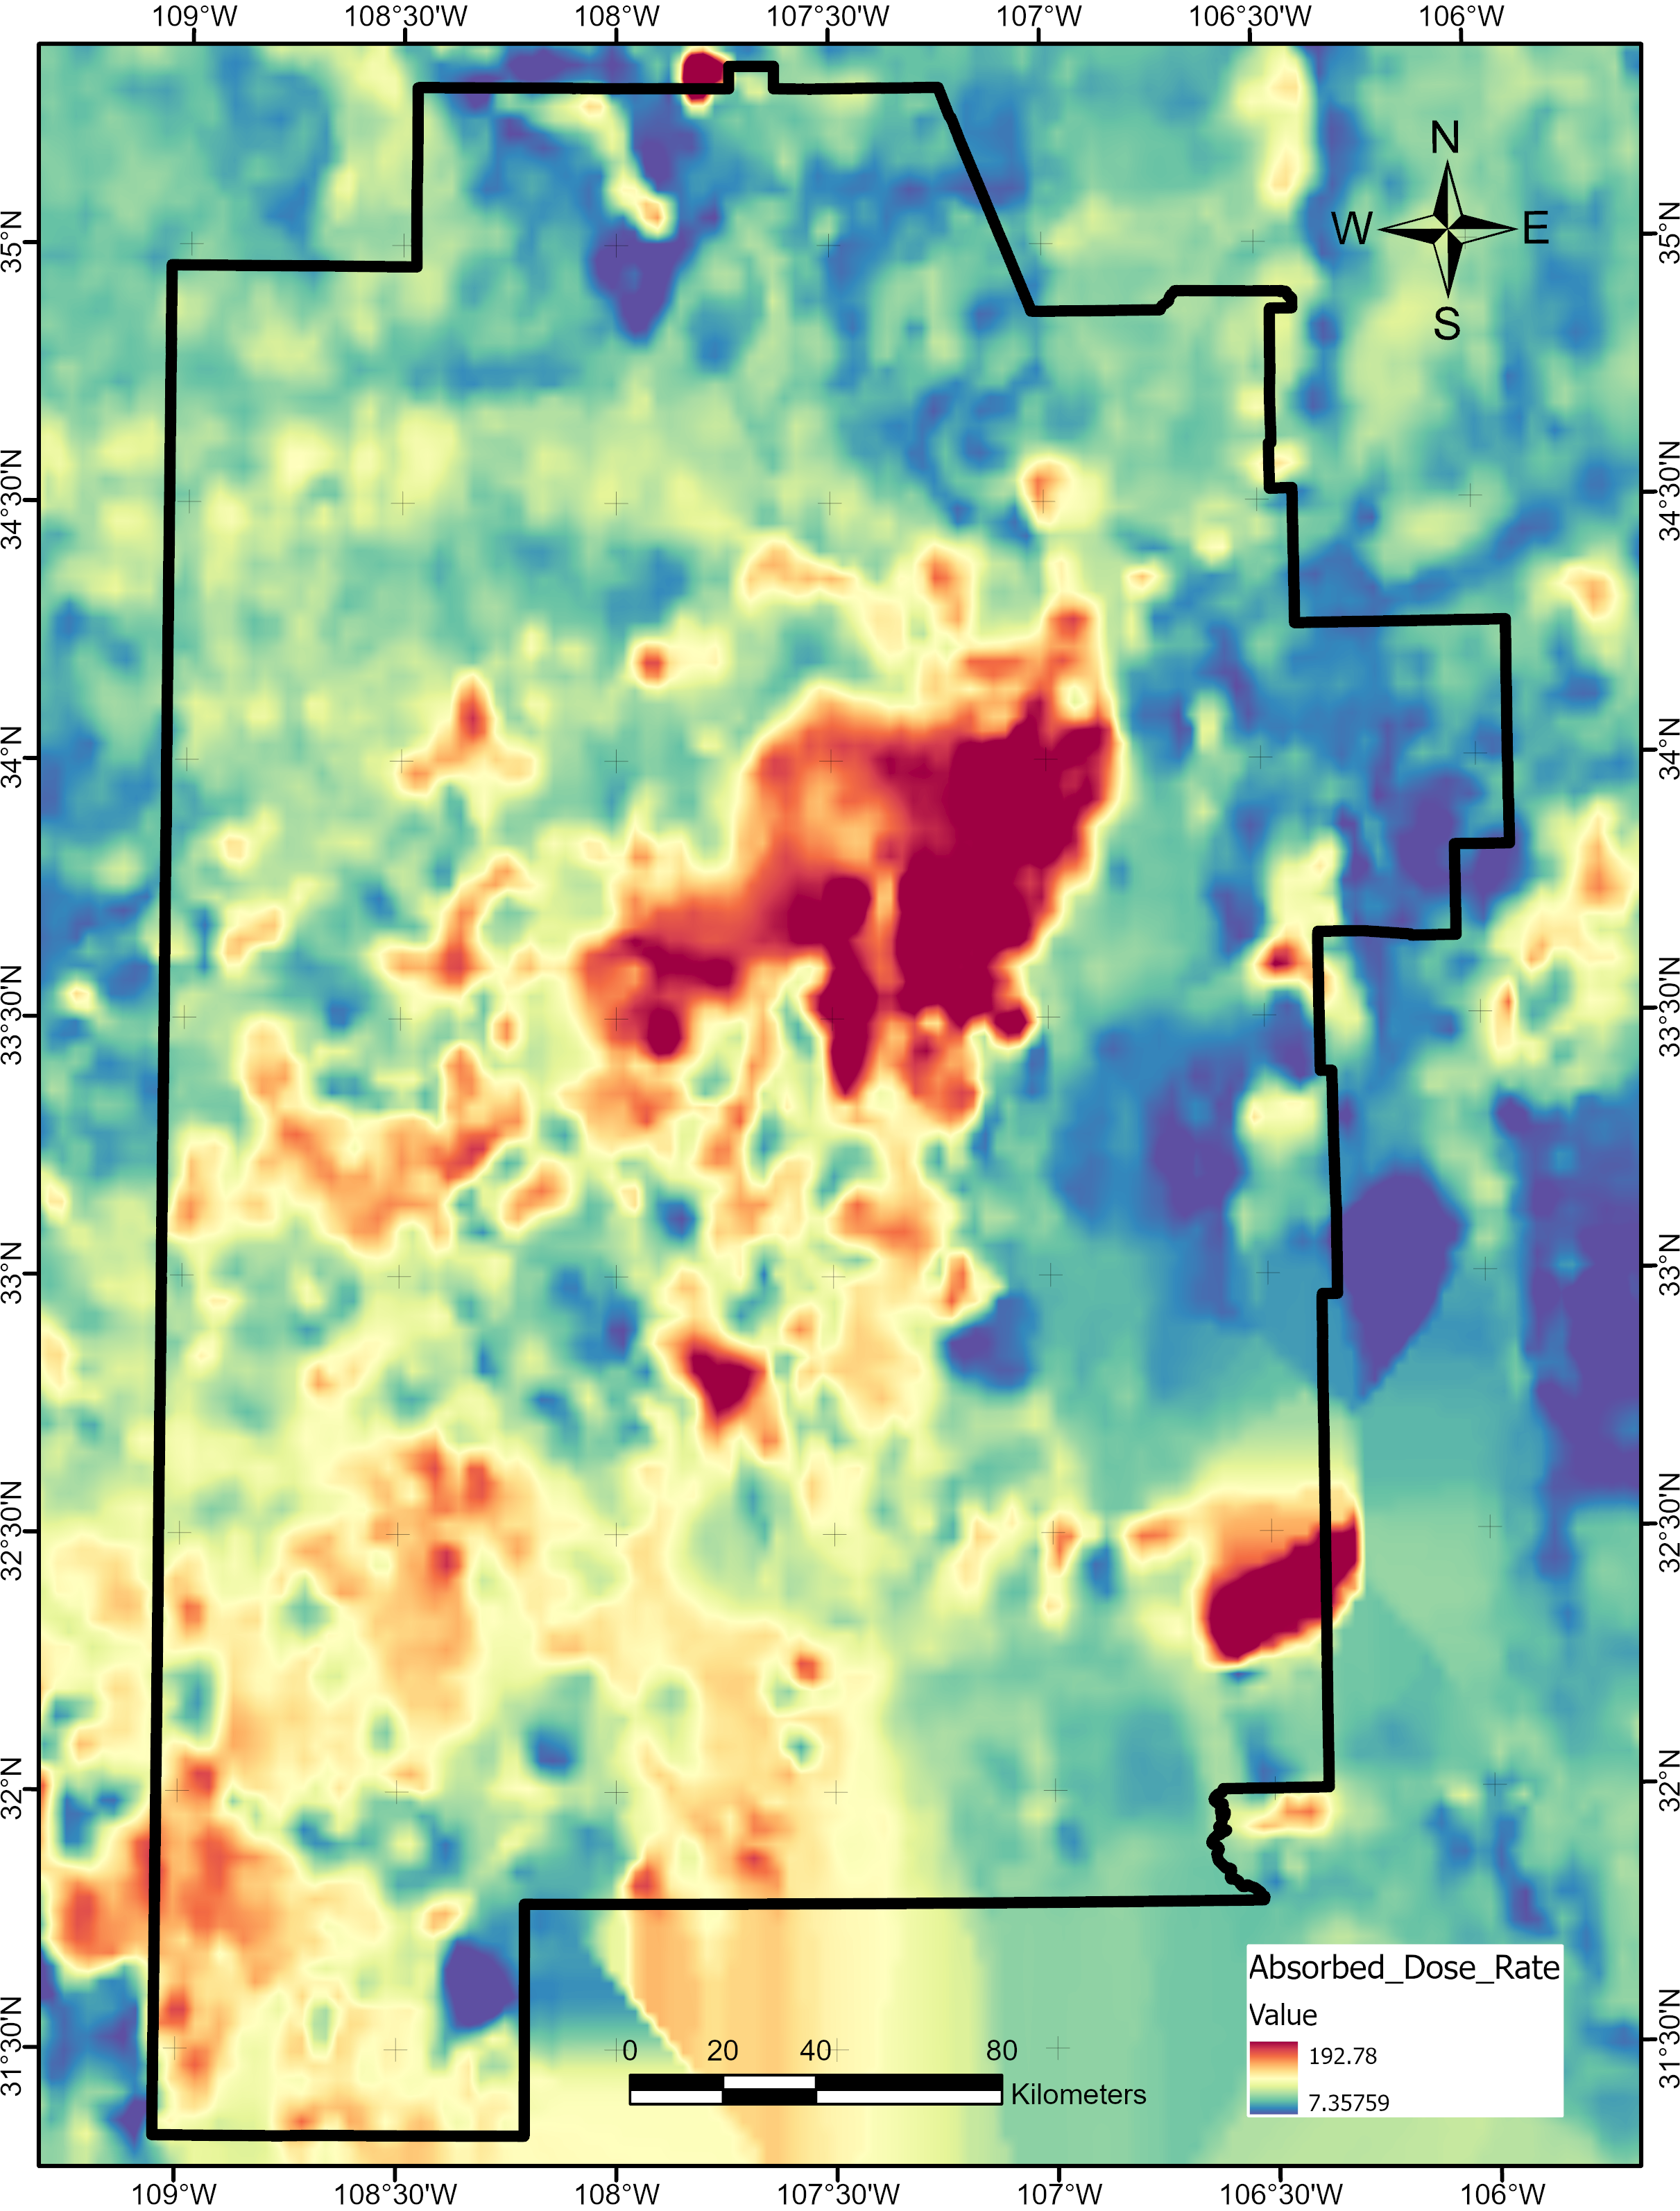
\includegraphics[scale=.50]{templates/images/Figure-AbsorbedDoseRate.png}
\caption[Absorbed dose rate data layer]{Absorbed dose rate data layer. Units are in nanoGrays/hour (nGy/hr). Original data from USGS Open-File Report 2005-1413 \protect\citep{duval_terrestrial_2005}}.
\label{fig:feat_gamma}
\end{figure}

\subsubsection{Geodetic Strain Rate}

GPS stations worldwide record local movements in the Earth’s crust. These movements can highlight inflation or subsidence of the surface, fault motions, or plate tectonic activity. The spatial derivative of crustal velocities is termed the strain rate, which gives an indication of the accumulation of strain in an area. More concretely, it defines the speed with which the crust is deforming, and can be treated as a proxy for earthquake potential since slip occurs due to the accumulation of strain \citep{gem_strain_2014}. The Global Strain Rate Model (GSRM) v.2.1 provides a model for strain rate based on over 22,000 measurements from over 18,000 locations around the world \citep{kreemer_geodetic_2014}. The output of this model was downloaded from the University of Nevada Reno Geodetic Laboratory host site \citep{kreemer_corne_global_2020}. GSRM describes elements of the full strain tensor at a resolution 0.1 degrees. The magnitude or second invariant of the strain tensor is defined as \citep{kreemer_geodetic_2014}:

\begin{equation}\label{eq:strainratemagnitude}
\left\lVert\dot{\epsilon}\right\rVert = \sqrt{\dot{\varepsilon}_{\phi\phi}^2+\dot{\varepsilon}_{\theta\theta}^2+2\dot{\varepsilon}_{\phi\theta}^2}
\end{equation}

Due to the size of the model file and complexity of this calculation, the data was first loaded into Python, cropped to the Extent Polygon bounds, and the strain rate magnitude was calculated for each point. These data were then loaded into ArcGIS and gridded using the \textit{Spline} function for a smooth interpolation of the coarser GSRM grid. The final layer (Figure \ref{fig:feat_strain}) was created using \textit{Spline} parameters: Regularized type, weight of 0.1, a 4-point requirement, and an output cell size of 0.025 degrees.

\begin{figure}[!htp]
\centering
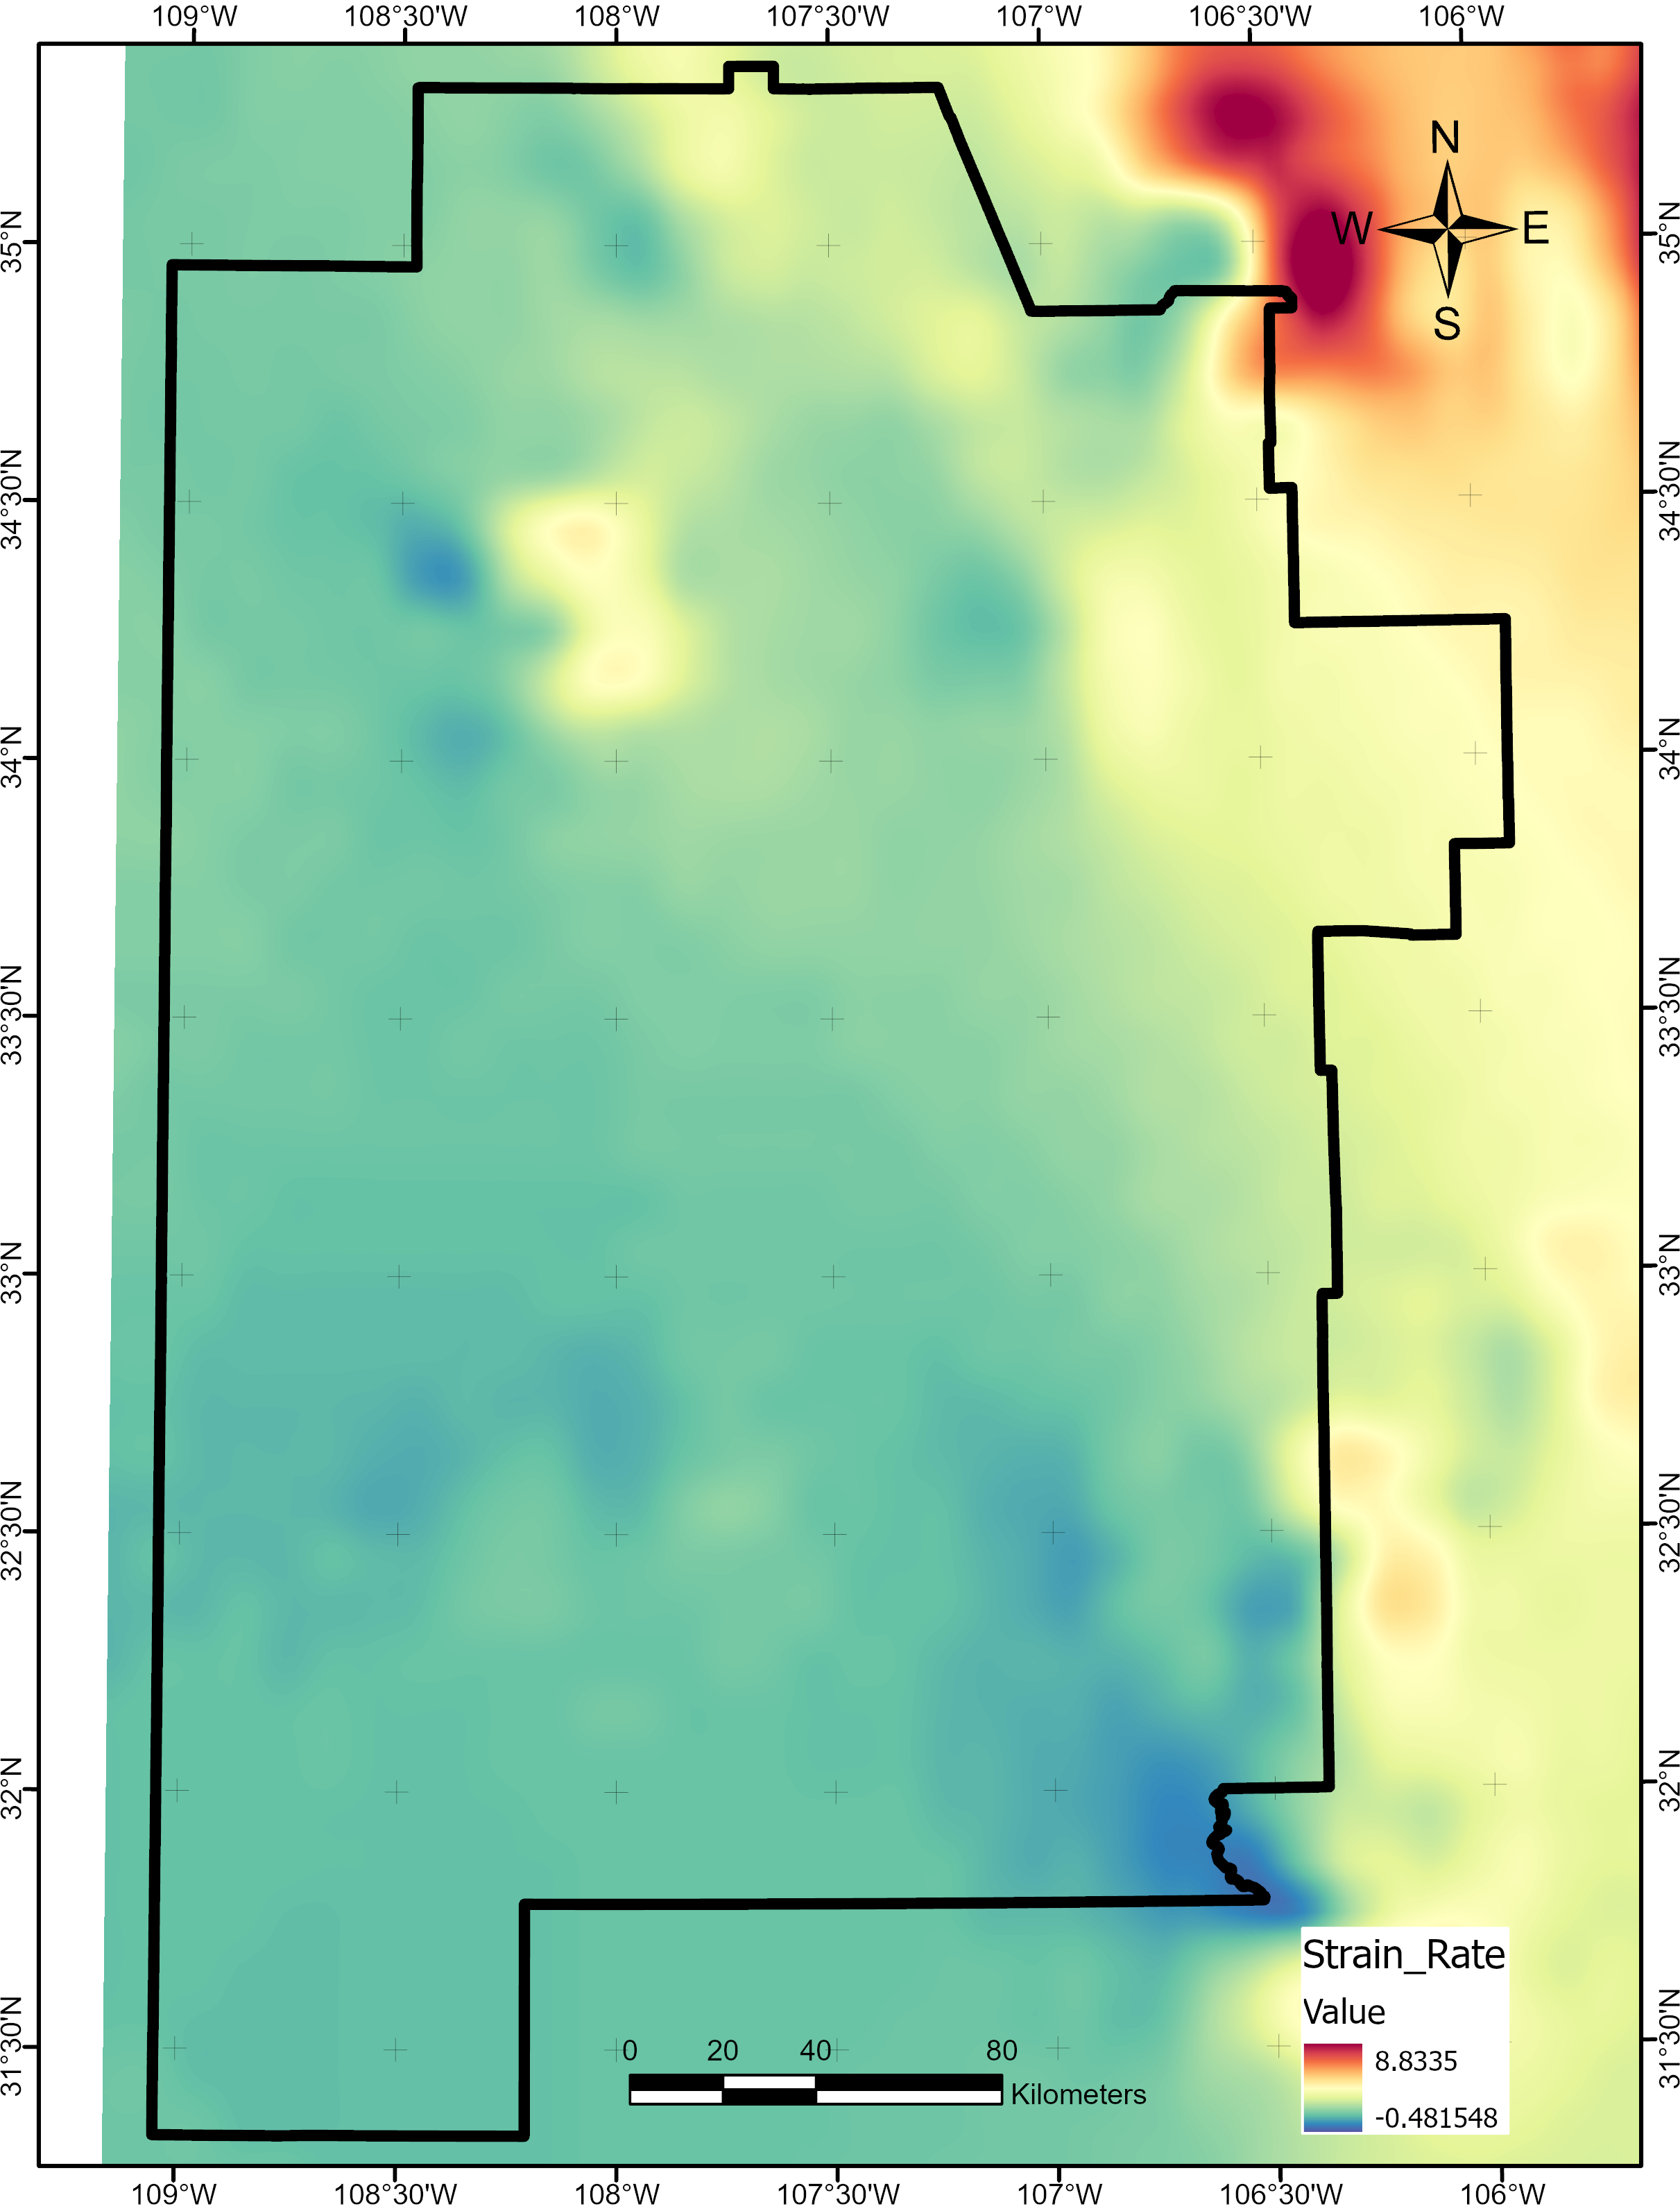
\includegraphics[scale=.50]{templates/images/Figure-StrainRate.png}
\caption[Geodetic strain rate data layer]{Geodetic strain rate data layer. Units are in \(10^-9 m/(m*yr)\). Layer is based on data from \protect\citep{kreemer_geodetic_2014}}.
\label{fig:feat_strain}
\end{figure}

\subsubsection{Gravity Anomaly}

Terrain-corrected gravity anomaly data available from the University of Texas El Paso \citep{utep_gravity_2011} were used in both the southwest NM PFA analysis \citep{bielicki_hydrogeolgic_2015} and cluster analysis \citep{pepin_new_2018}. The data layer from \citeauthor{bielicki_hydrogeolgic_2015} was downloaded from their OpenEI submission \citep{kelley_geothermal_2015} and loaded into ArcGIS. The layer (Figure \ref{fig:feat_gravity}) required no further processing.

\begin{figure}[!htp]
\centering
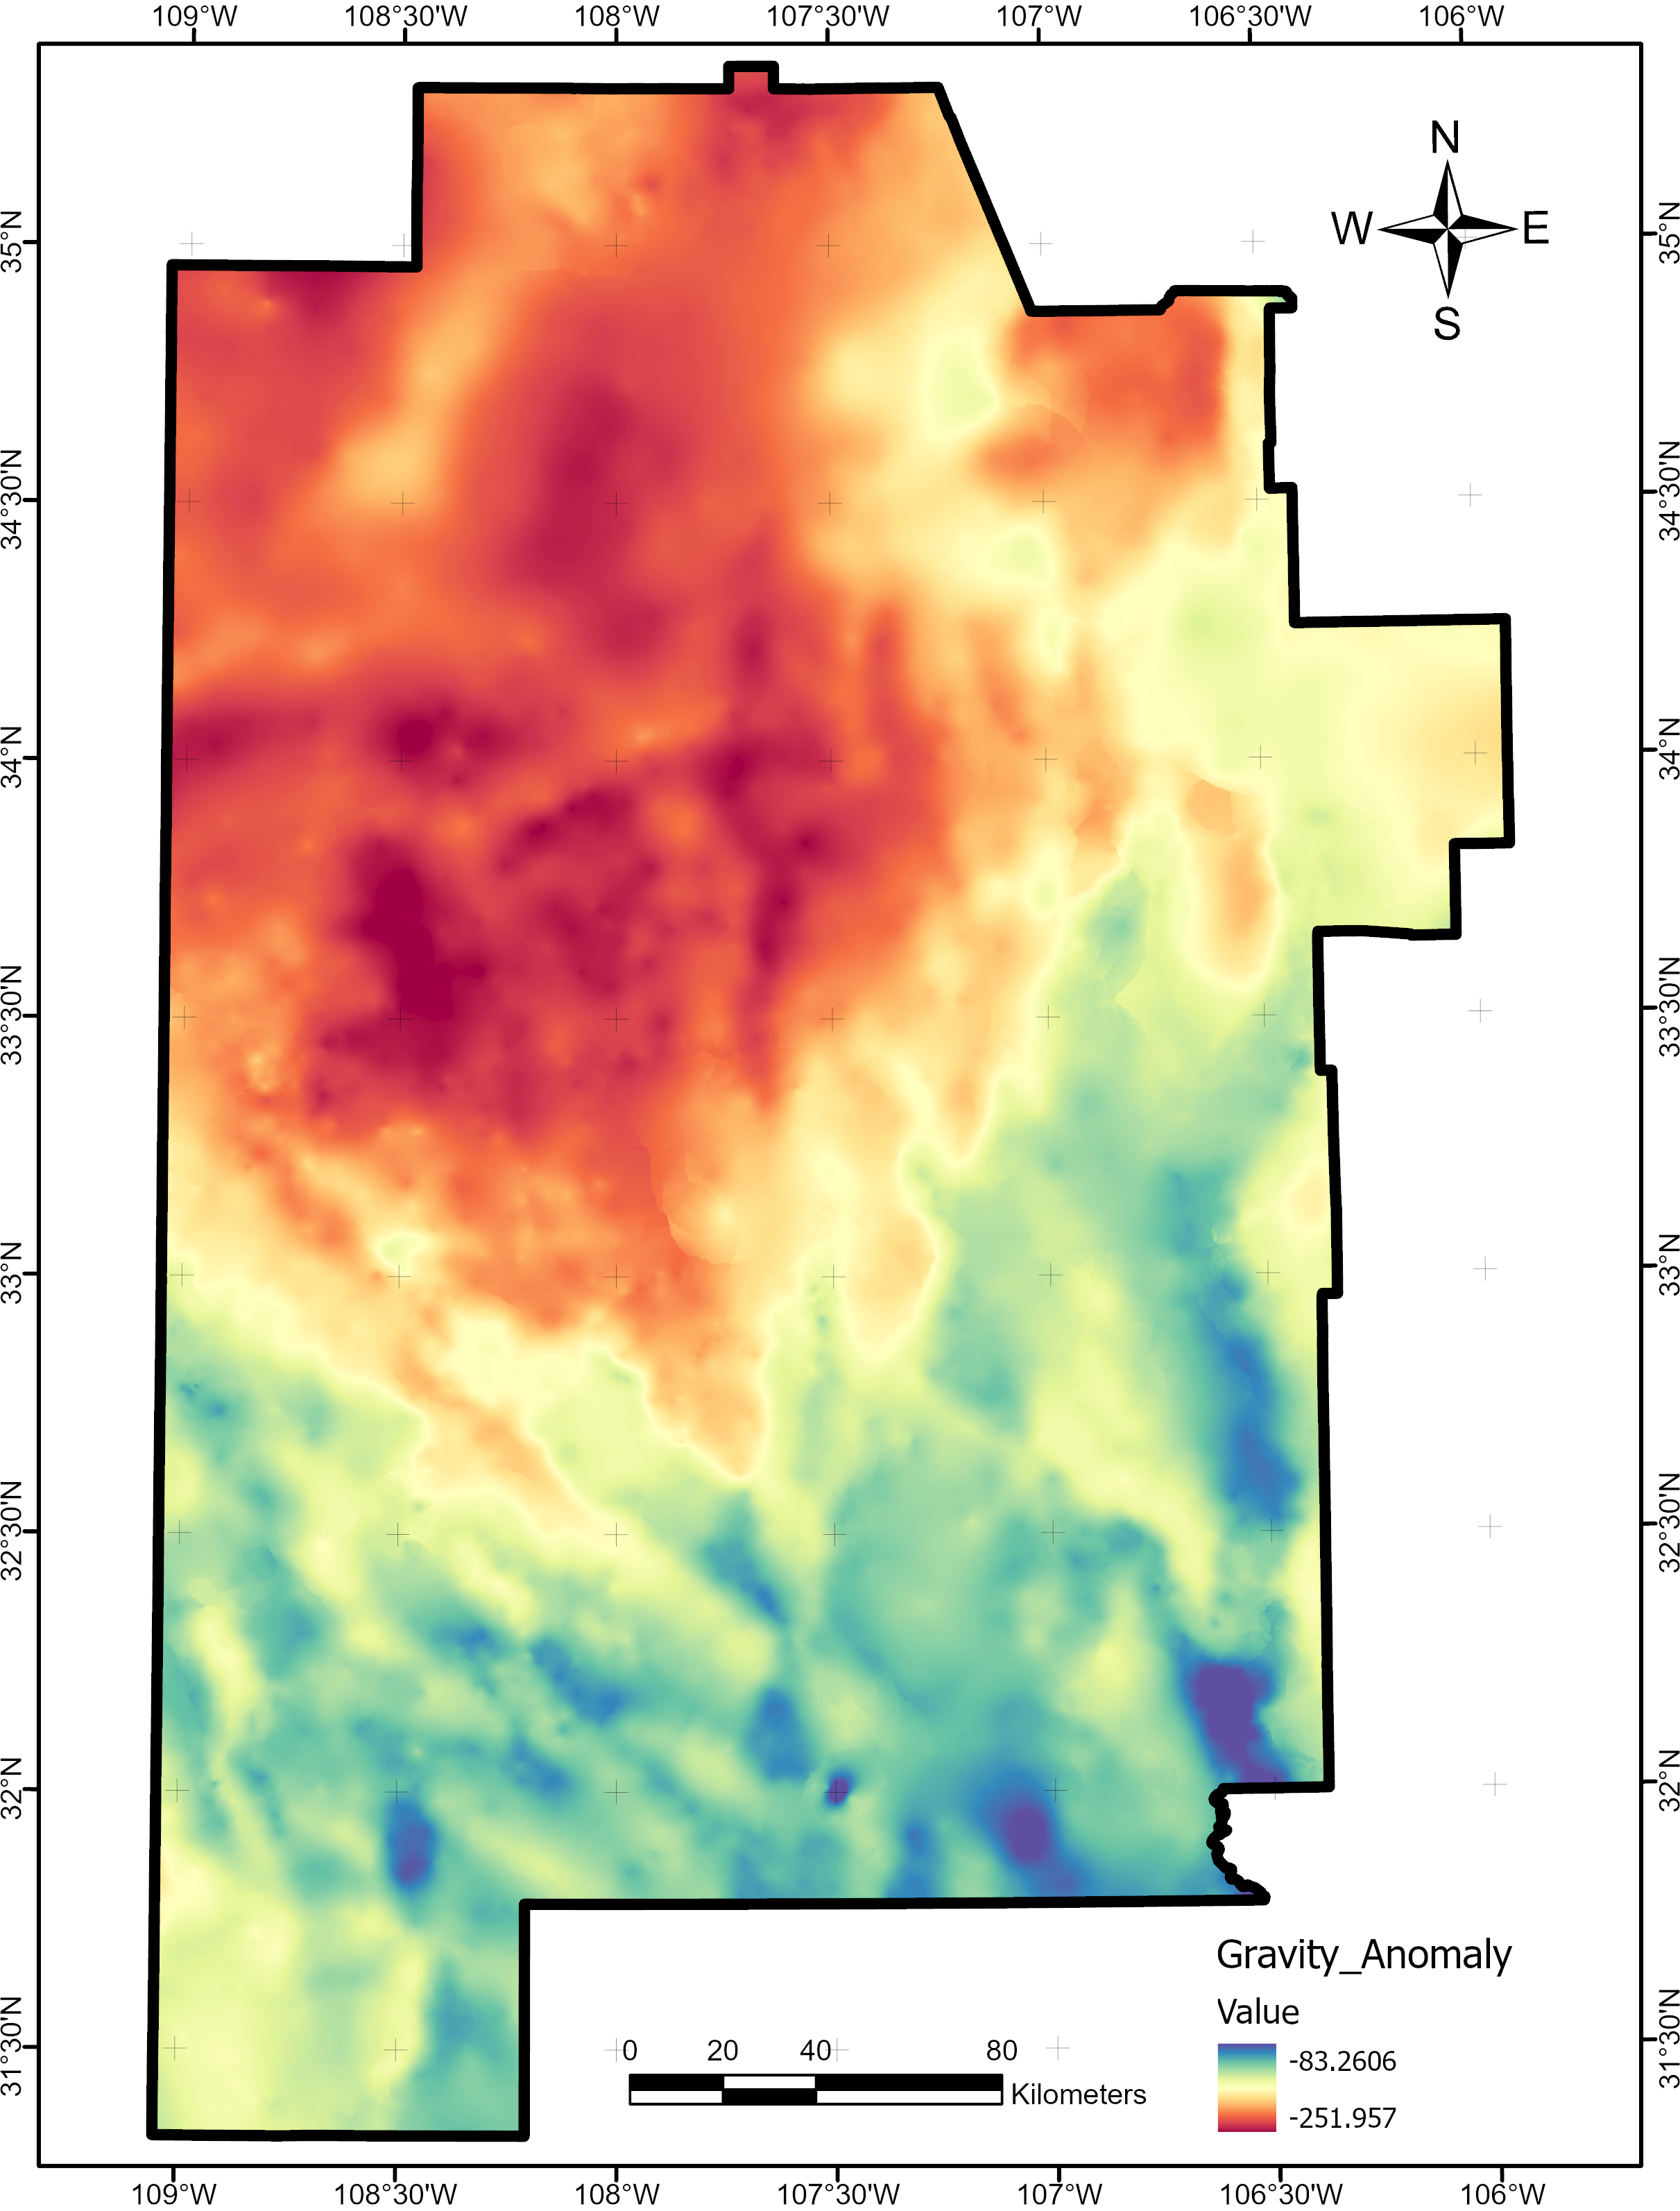
\includegraphics[scale=.50]{templates/images/Figure-GravityAnomaly.png}
\caption[Gravity anomaly data layer]{Gravity anomaly data layer. Units are in milligals (mGal). Raster originally created by \protect\citet{bielicki_hydrogeolgic_2015}.}.
\label{fig:feat_gravity}
\end{figure}

\subsubsection{Gravity Anomaly Gradient}

Gradient of the gravity anomaly was calculated using the ArcGIS Slope function on the final gravity anomaly raster. Parameters used to create the final layer (Figure \ref{fig:feat_gravity_gradient} include: Geodesic method, Z unit of meters, and output measurement of degrees.

\begin{figure}[!htp]
\centering
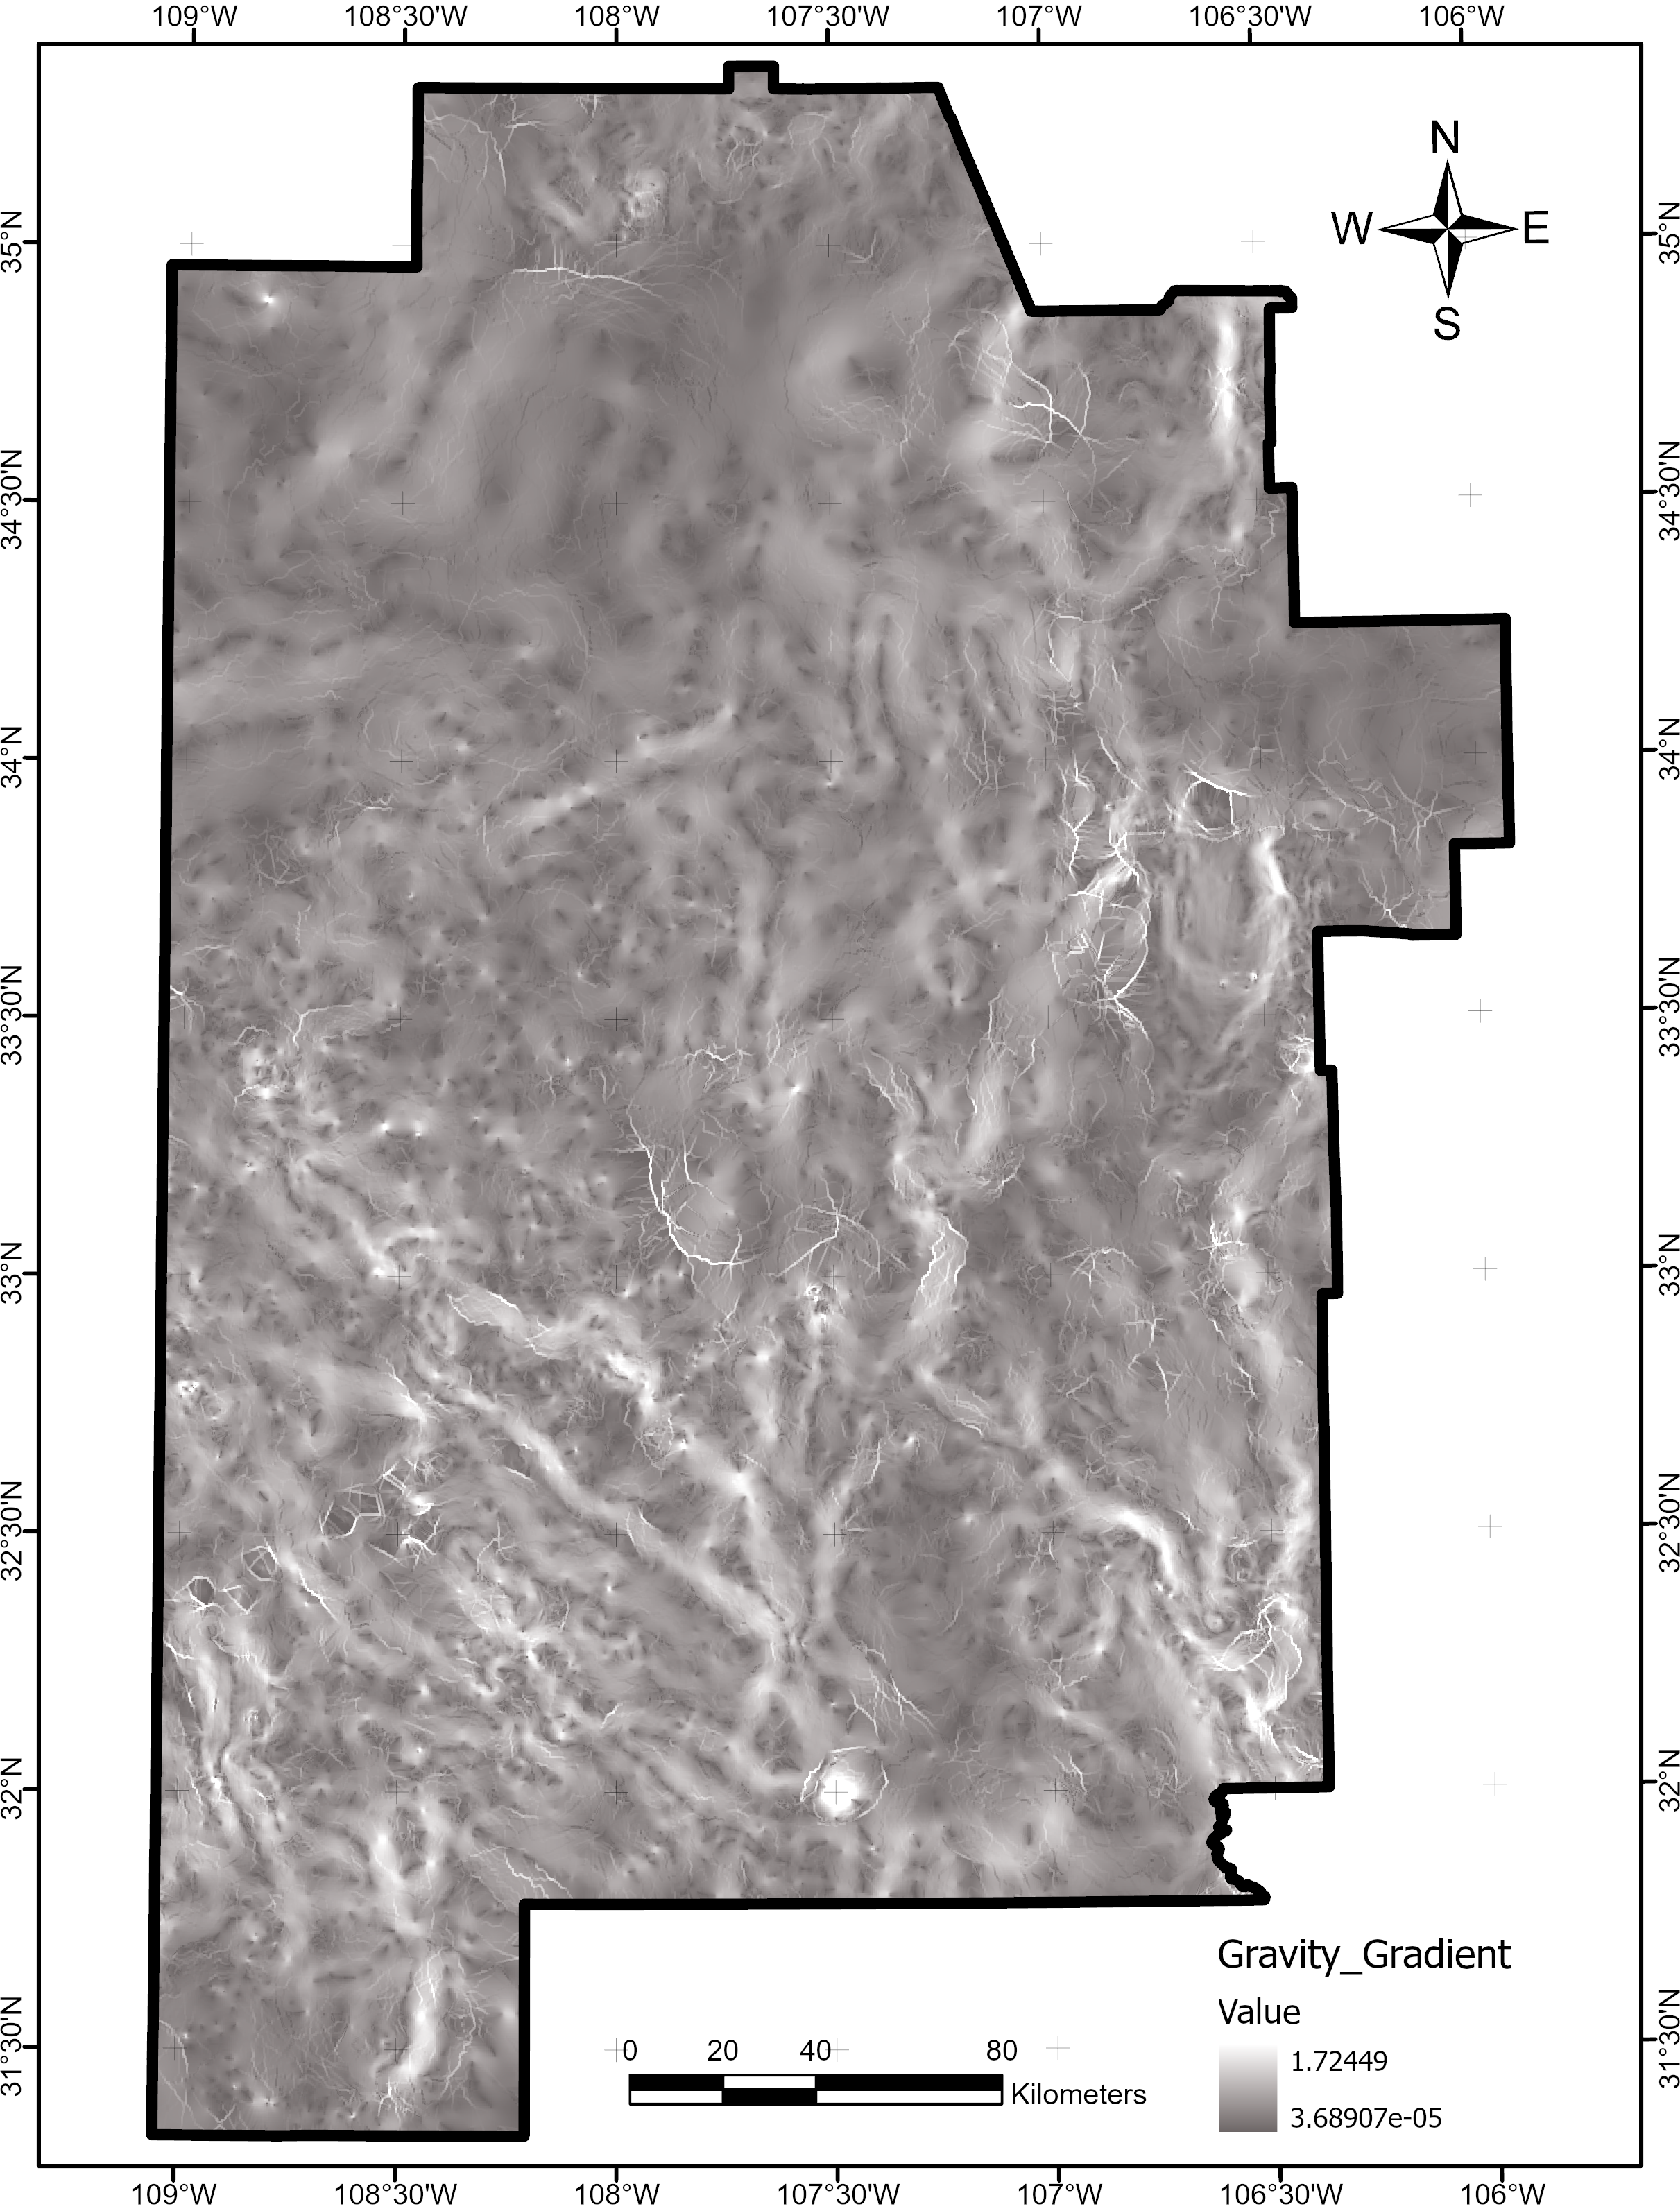
\includegraphics[scale=.50]{templates/images/Figure-GravityGradient.png}
\caption[Gravity anomaly gradient data layer]{Gravity anomaly gradient data layer. Units are in mGal/degrees.}.
\label{fig:feat_gravity_gradient}
\end{figure}

\subsubsection{Heat Flow}

The recent $0.5^\circ$ x$0.5^\circ$ resolution heat flow model from \citet{lucazeau_analysis_2019} offers coarse coverage across the southwest NM AOI. The model output was downloaded from the supporting information section of the publication page \citep{lucazeau_analysis_2019}, loaded into ArcGIS, and cropped to the Extent Polygon boundaries. After testing several gridding algorithms for a smooth representation of this sparse data, the ArcGIS \textit{Topo to Raster} function produced the best results. The final layer (Figure \ref{fig:feat_heatflow}) parameters include: tolerance 1 of 2.5, tolerance 2 of 100, drainage enforcement set to Enforce, Contour selected for primary type of input data, and output cell size of 0.01. 

\begin{figure}[!htp]
\centering
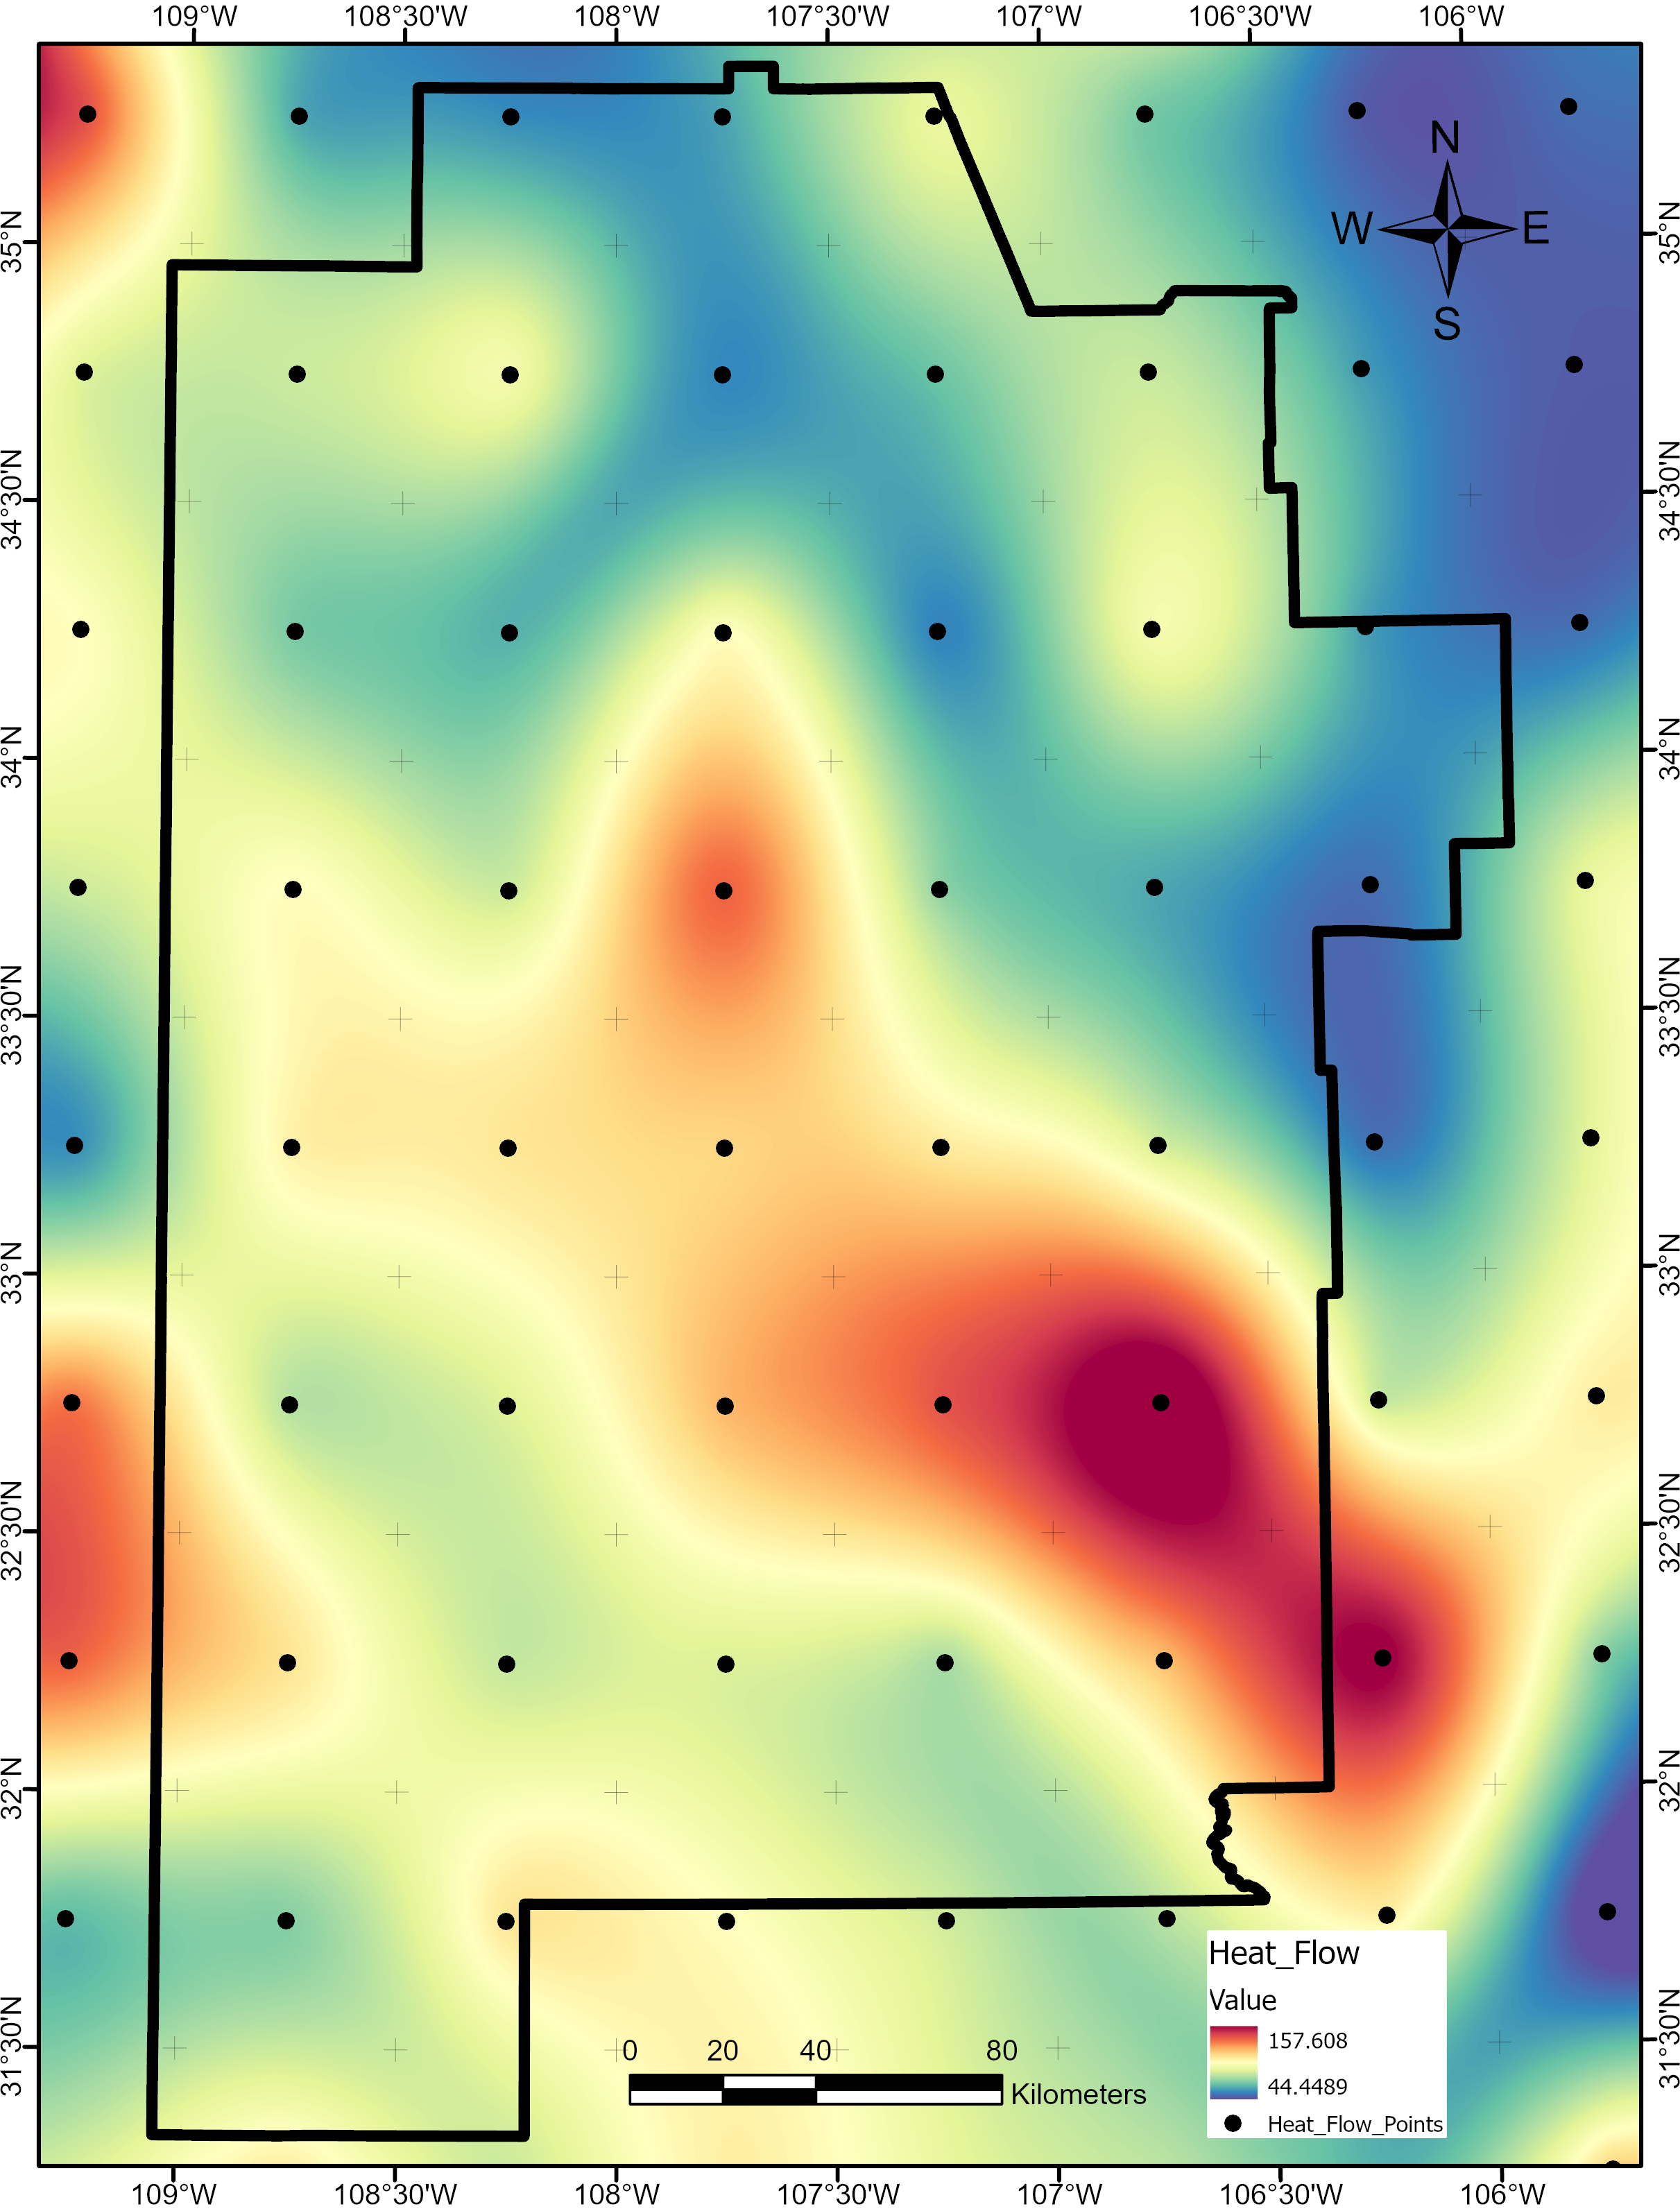
\includegraphics[scale=.50]{templates/images/Figure-HeatFlow.png}
\caption[Heat flow data layer]{Heat flow data layer. Units are in W/m-K. Original data from \protect\citep{lucazeau_analysis_2019}.}.
\label{fig:feat_heatflow}
\end{figure}

\subsubsection{Lithium Concentration}

Measurements of Lithium concentration were originally assembled by \citet{bielicki_hydrogeolgic_2015} from several sources ranging from USGS records to student dissertations. These data were downloaded from the OpenEI submission \citep{kelley_geothermal_2015} and merged together using ArcGIS and Python to create a single dataframe of 3595 measurements, all within the broader Extent Polygon bounds to avoid surface creation edge effects within the tighter AOI. As described for the Boron concentration data layer, attempts to model Lithium concentration using Gaussian Processes provided unsatisfactory results. Instead, the final layer was generated using the ArcGIS \textit{Empirical Bayes Kriging} routine. Selected parameters include: Empirical data transformation type, a maximum of 100 points in each local model, 100 simulated semivariograms with K-Bessel model type, and a standard circular search neighborhood with a radius of 1.1957 (auto-generated), minimum of 10 neighbors, and maximum of 15 neighbors. The output grid cell size was set to 0.01 degrees. All coincident data was included in the calculation, so any overlapping measurements were considered in generating the final layer (Figure \ref{fig:feat_lithium}).

\begin{figure}[!htp]
\centering
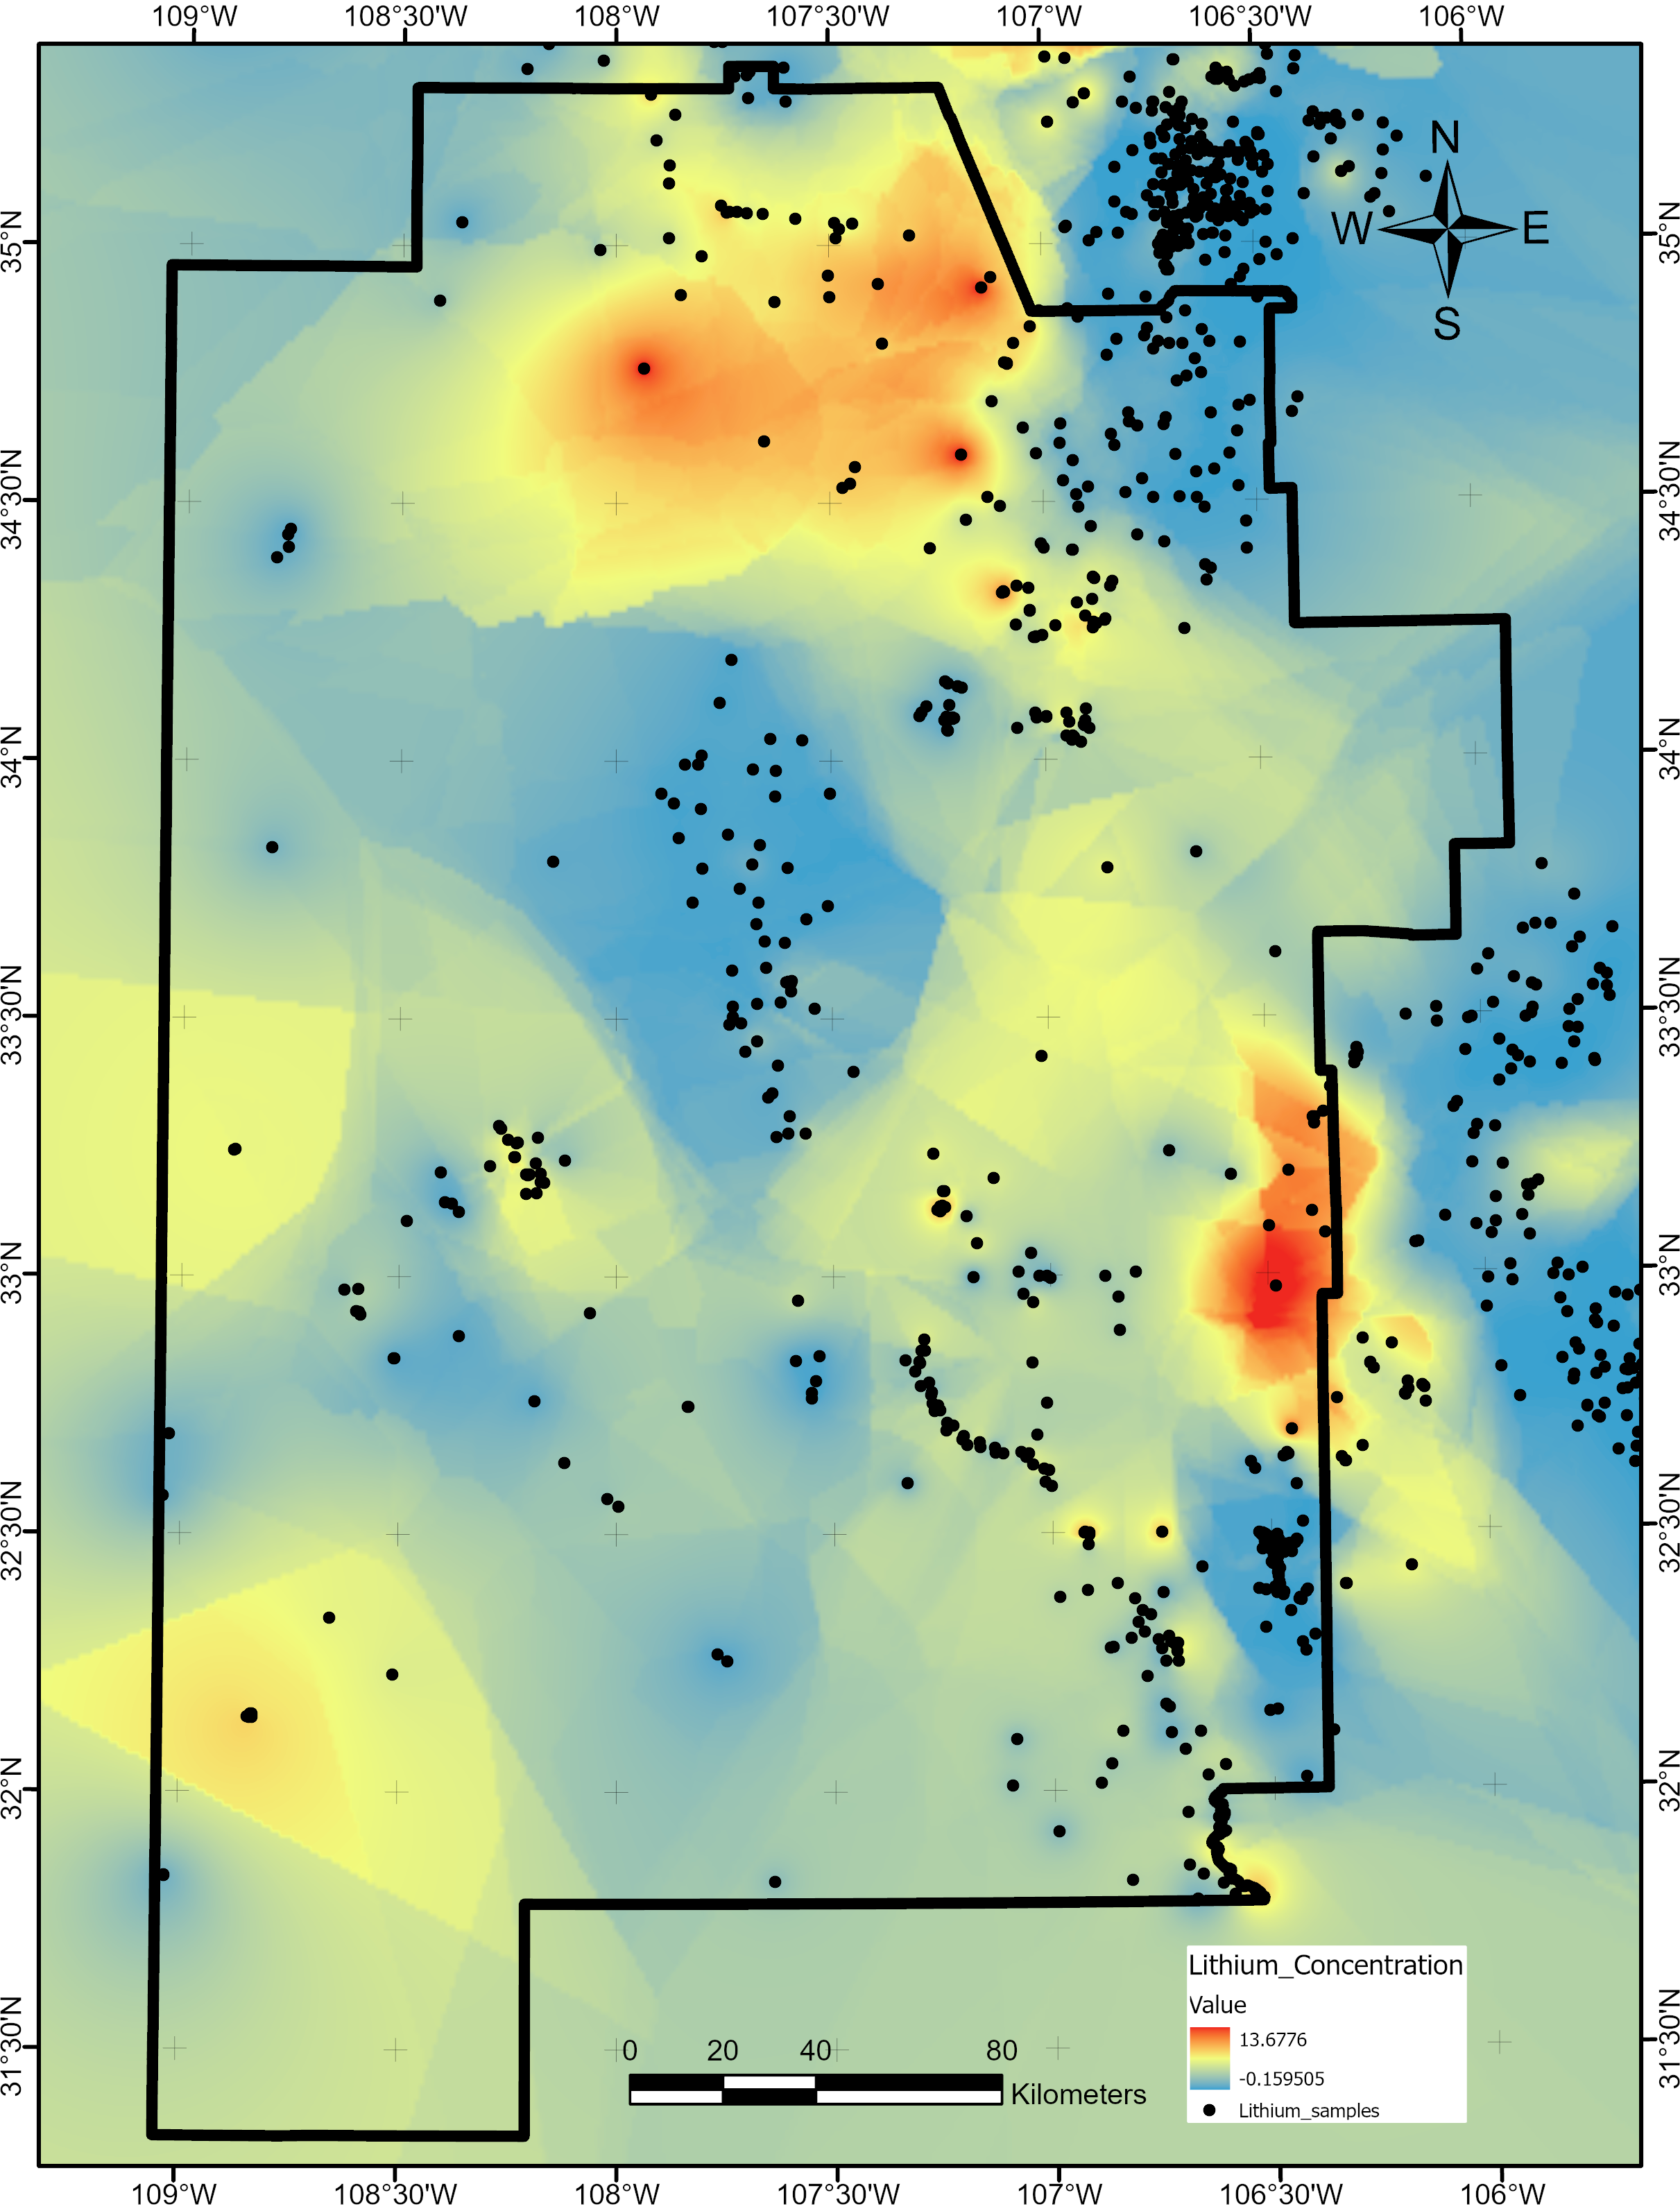
\includegraphics[scale=.50]{templates/images/Figure-Lithium.png}
\caption[Lithium concentration data layer]{Lithium concentration data layer. Units in ppm or mg/L. Black dots indicate sample locations in complete data set from \protect\citep{bielicki_hydrogeolgic_2015}}.
\label{fig:feat_lithium}
\end{figure}

\subsubsection{Magnetic Anomaly}

USGS magnetic anomaly data derived from aerial surveys \citep{bankey_digital_2002} were used in both the southwest NM PFA analysis \citep{bielicki_hydrogeolgic_2015} and cluster analysis \citep{pepin_new_2018}. After downloading the raster from the southwest NM PFA OpenEI submission \citep{kelley_geothermal_2015}, it was loaded into ArcGIS. The layer (Figure \ref{fig:feat_magnetics}) required no further processing.

\begin{figure}[!htp]
\centering
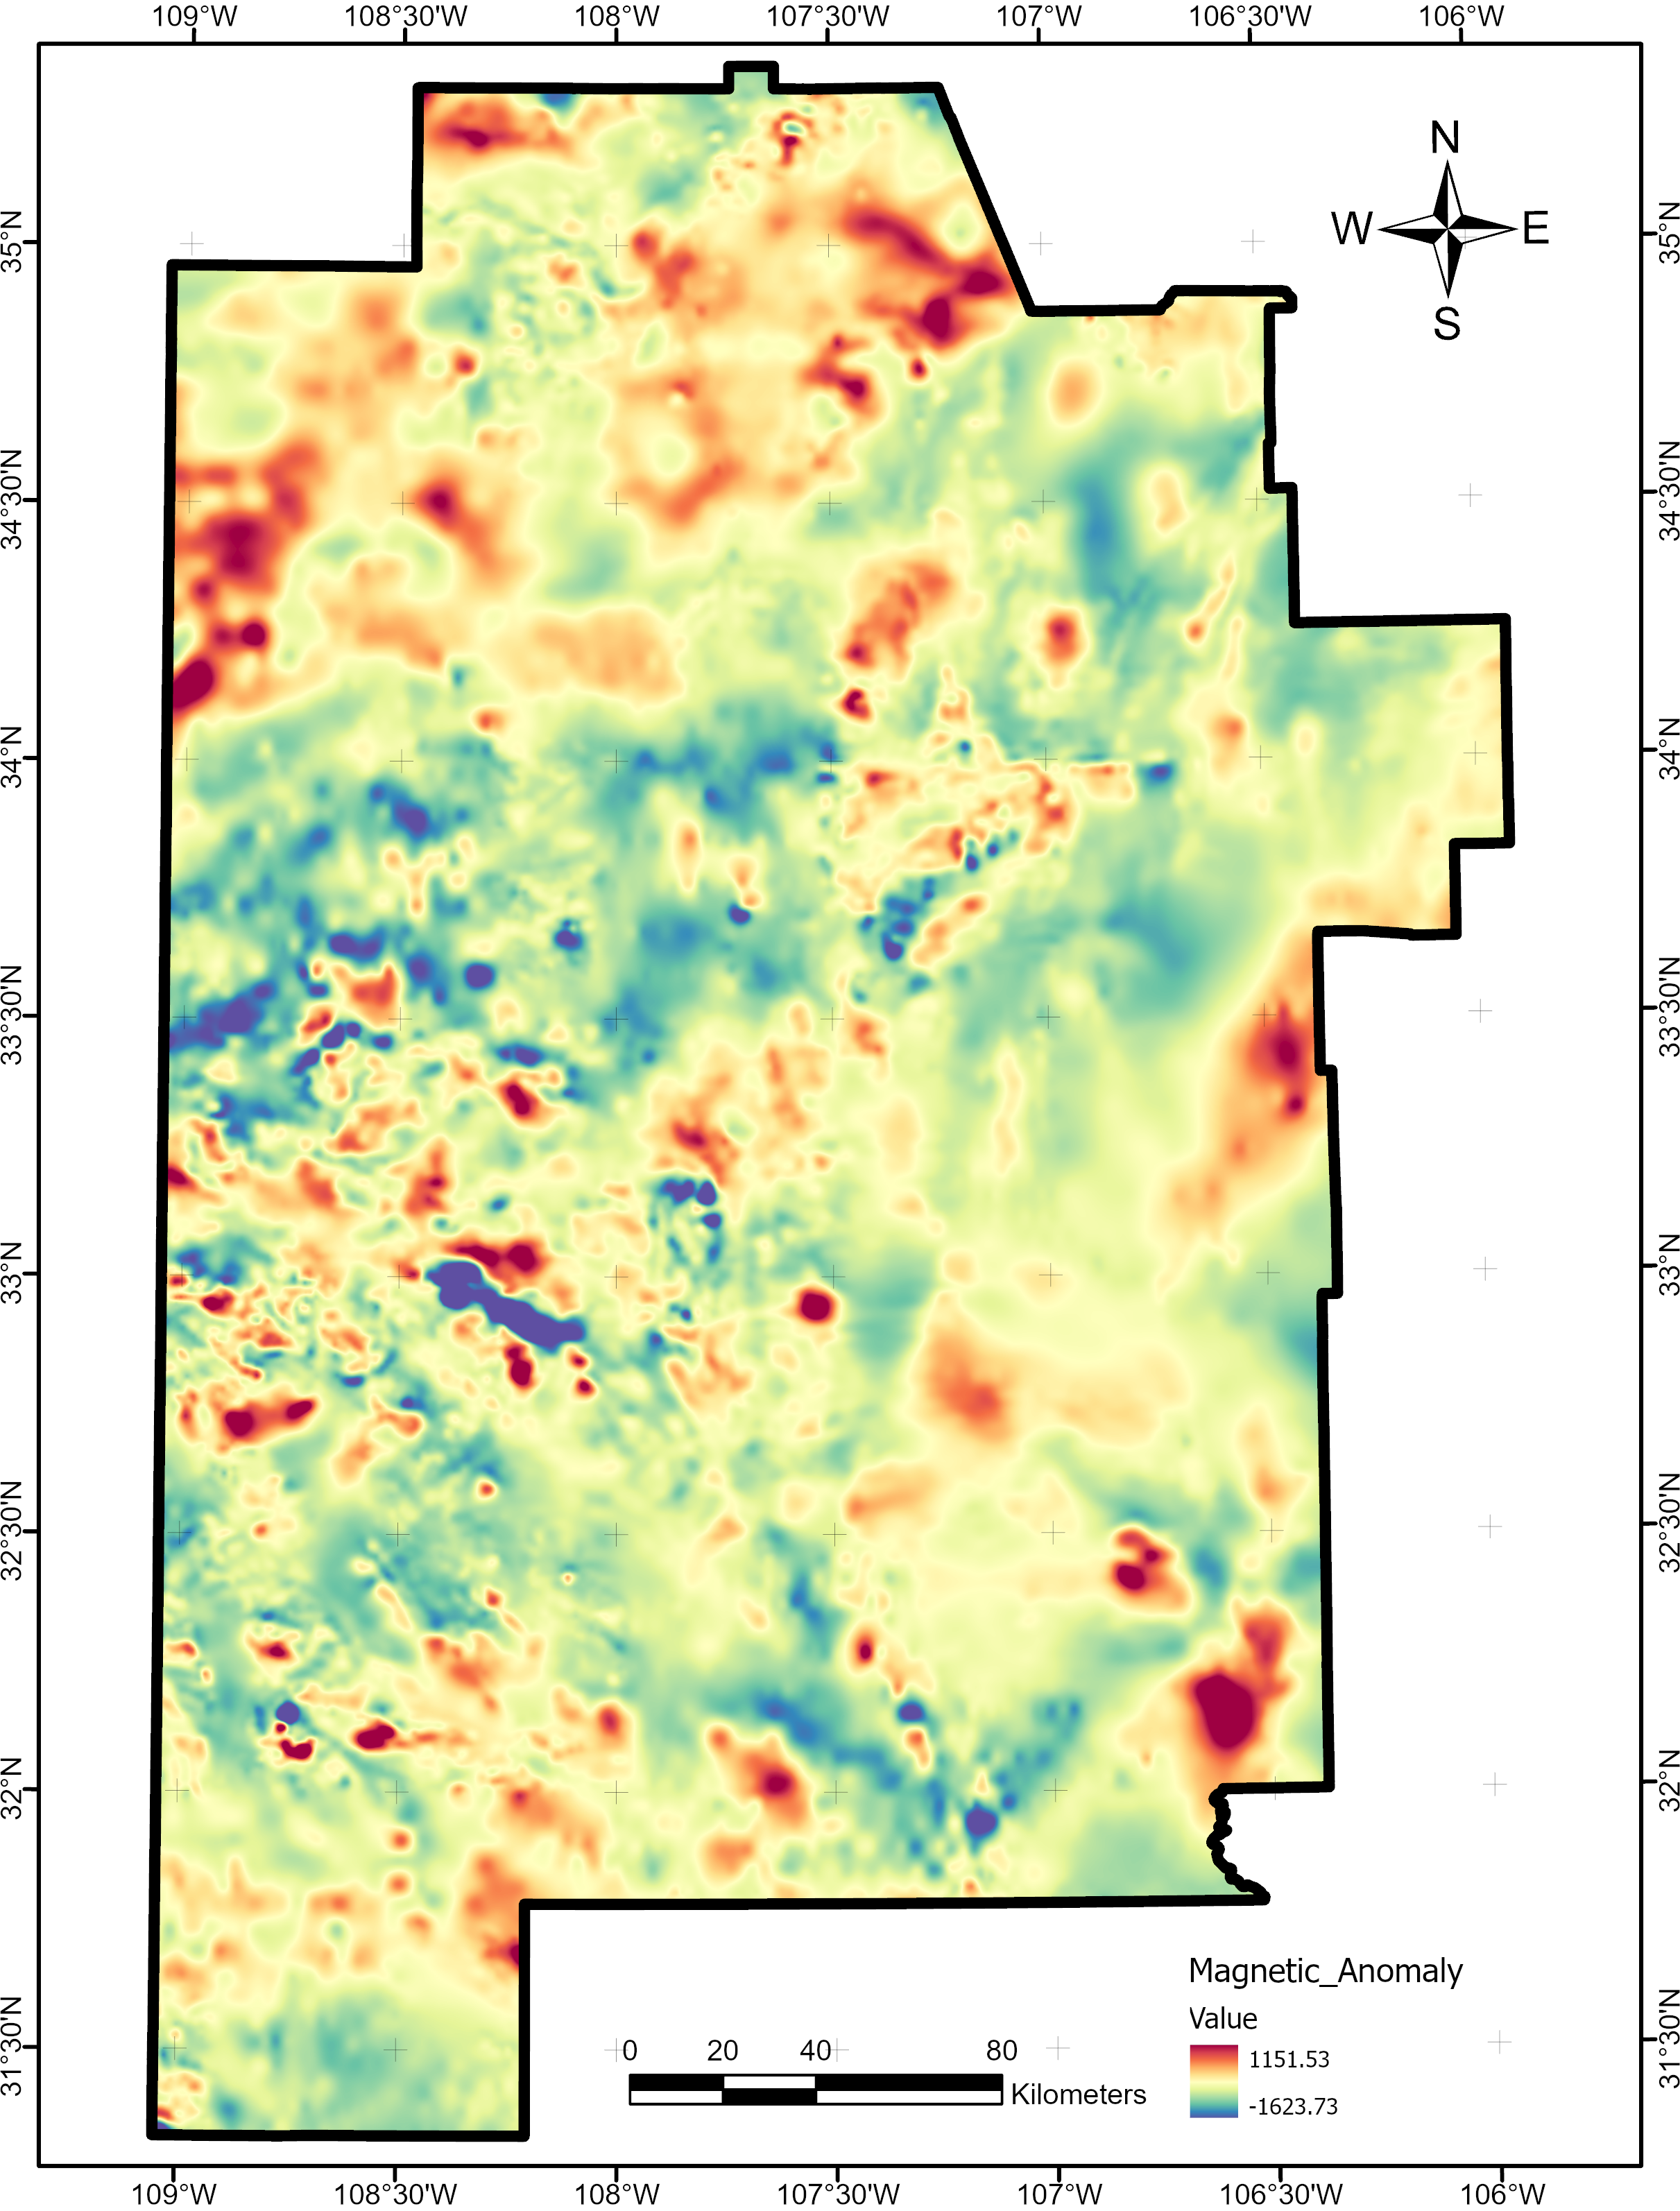
\includegraphics[scale=.50]{templates/images/Figure-MagneticAnomaly.png}
\caption[Magnetic anomaly data layer]{Magnetic anomaly data layer. Units are in nanoteslas (nT). Raster originally created by \protect\citet{bielicki_hydrogeolgic_2015}.}.
\label{fig:feat_magnetics}
\end{figure}

\subsubsection{Magnetic Anomaly Gradient}

The gradient of the magnetic anomaly was calculated using the ArcGIS Slope function on the final magnetic anomaly raster. Parameters used to create the final layer (Figure \ref{fig:feat_magnetic_gradient}) include: Geodesic method, Z unit of meters, and output measurement of degrees.

\begin{figure}[!htp]
\centering
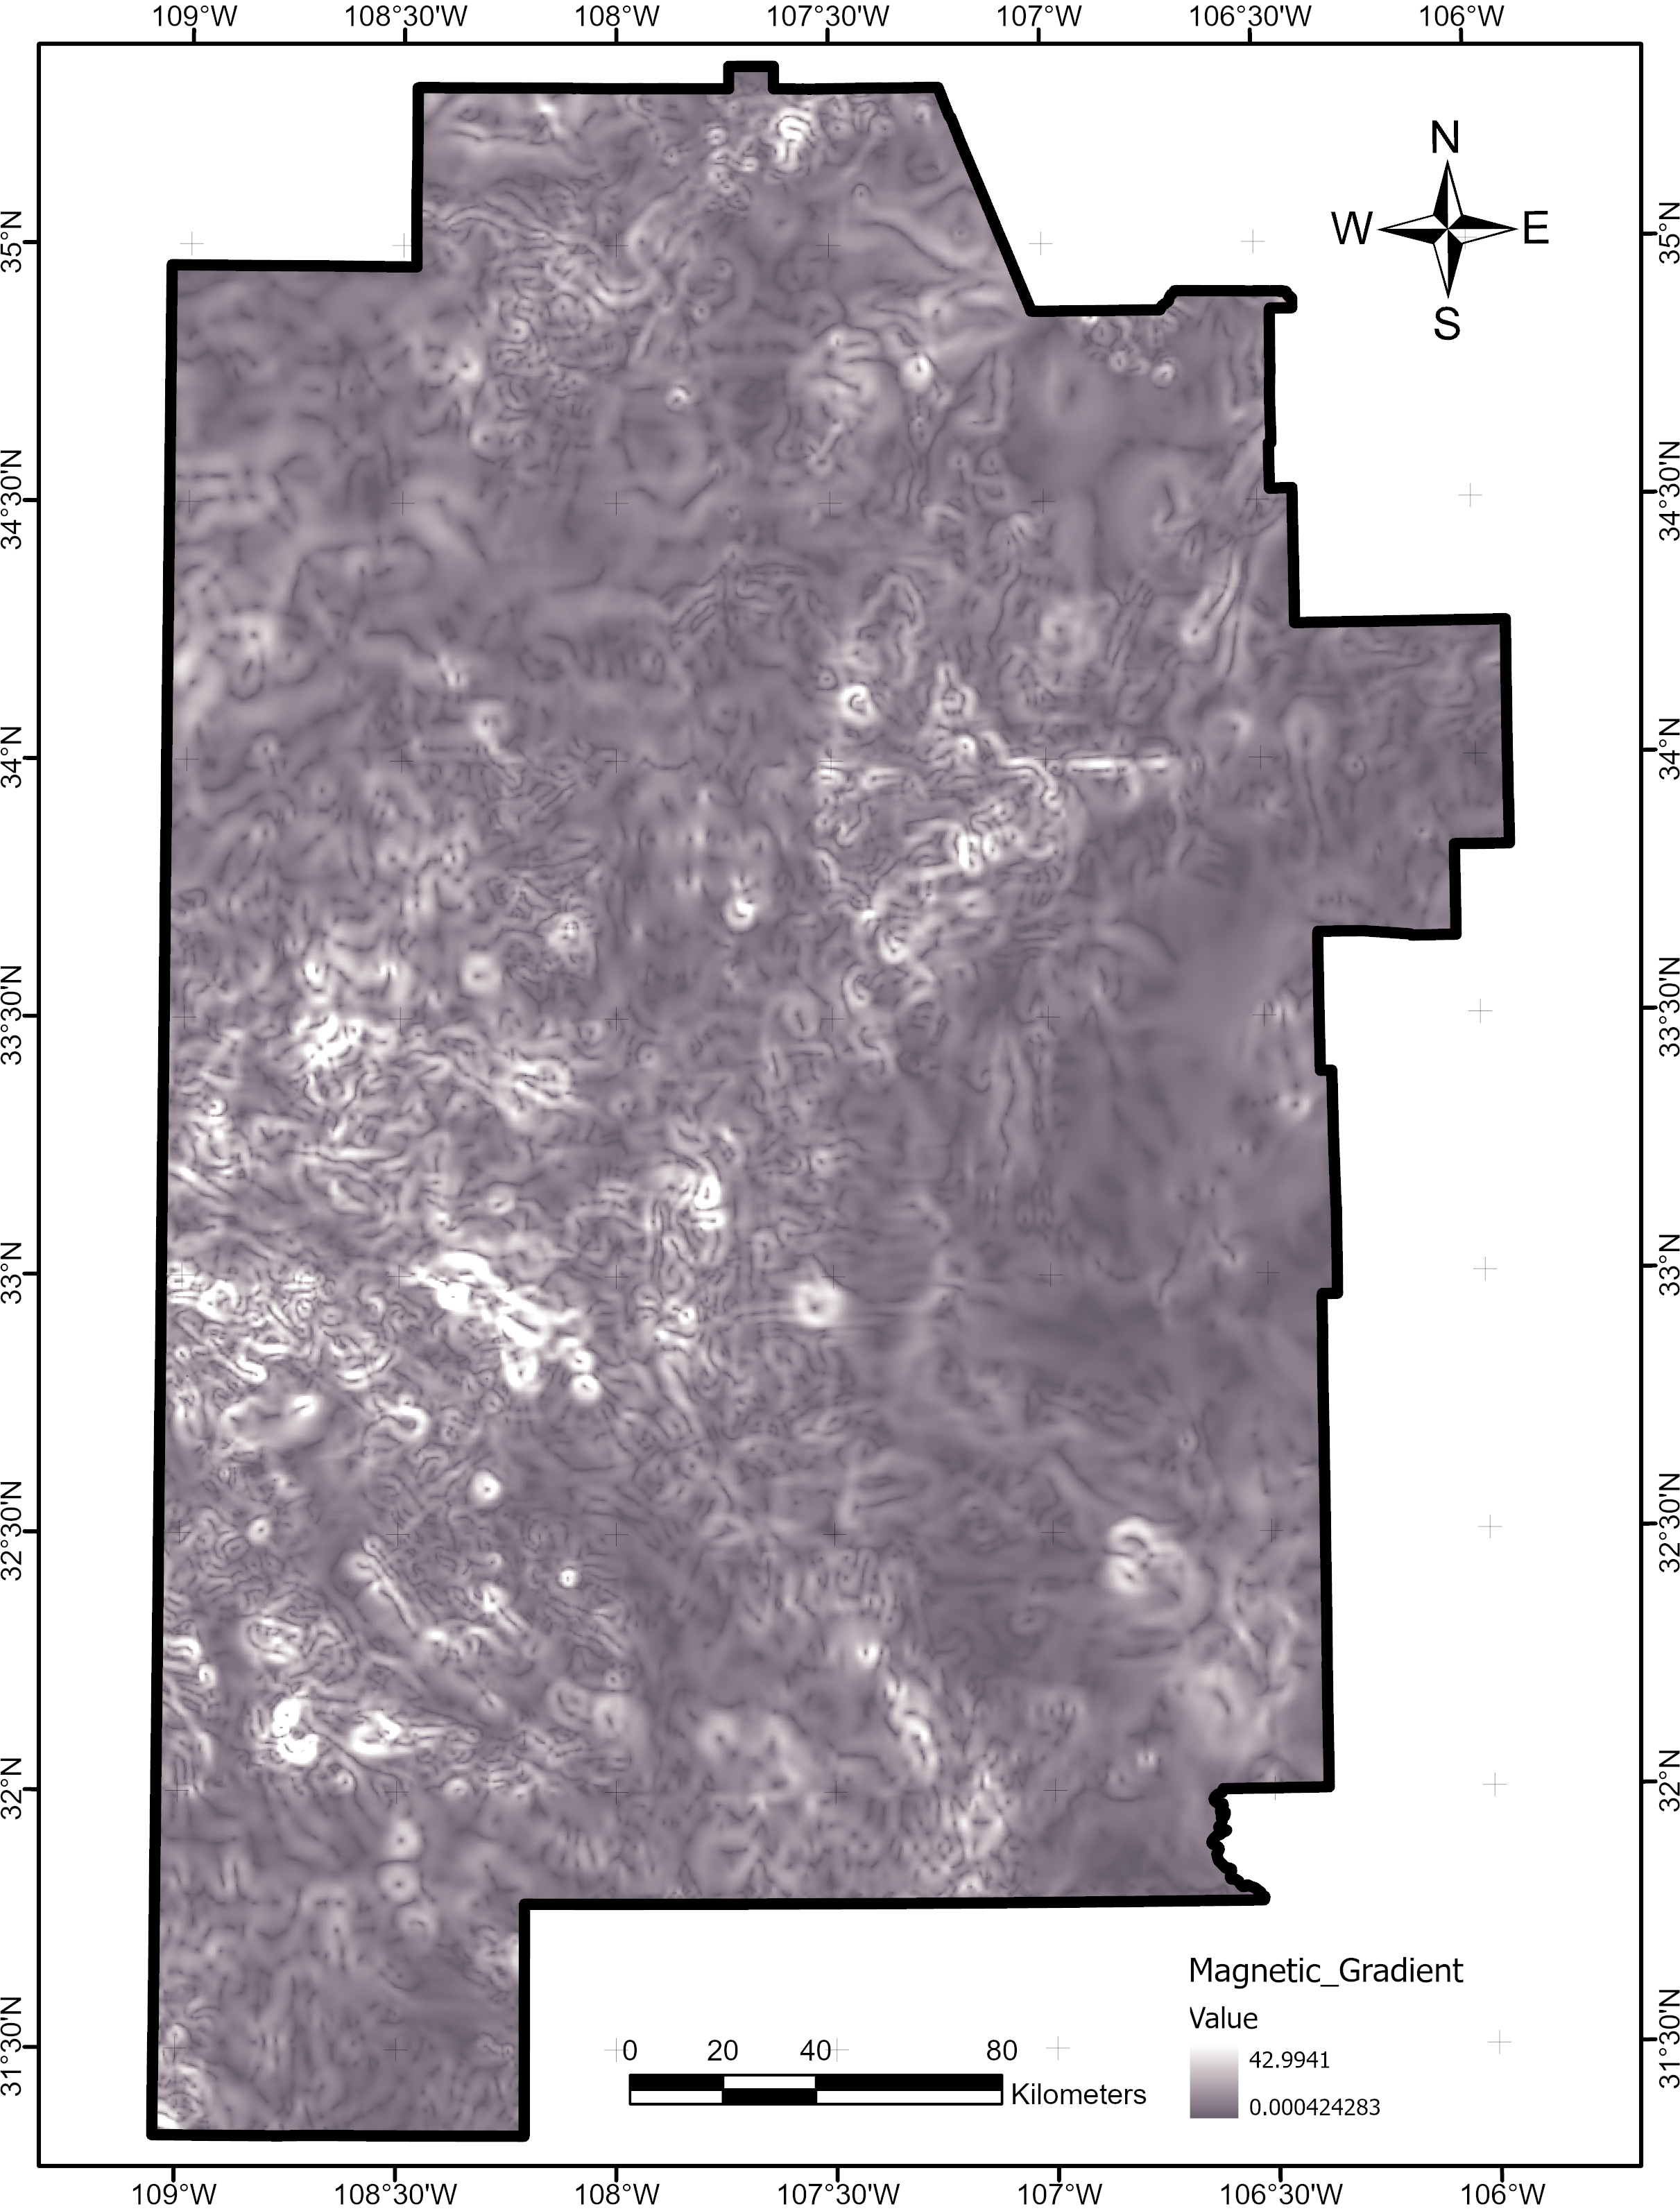
\includegraphics[scale=.50]{templates/images/Figure-MagneticGradient.png}
\caption[Magnetic anomaly gradient data layer]{Magnetic anomaly gradient data layer. Units are in nT/degrees.}.
\label{fig:feat_magnetic_gradient}
\end{figure}

\subsubsection{Quaternary Fault Density}

Faults showing Quaternary displacement were digitized at the 1:24,000 scale by the New Mexico Bureau of Geology and Mineral Resources and provided by NM BGMR to \citet{bielicki_hydrogeolgic_2015} and \citet{pepin_new_2018} in support of their investigations. The associated polyline features were downloaded from the PFA OpenEI submission \citep{kelley_geothermal_2015} and loaded into ArcGIS. As discussed for the Drainage density layer, a Python-based kernel density workflow using extracted points from these polylines failed to produce satisfactory results. Instead, the ArcGIS \textit{Kernel Density} function was applied to create the final layer map (Figure \ref{fig:feat_qfaults}). Selected parameters for this function include an output cell size of 0.0025 degrees and an auto-generated search radius of 0.3672.

\begin{figure}[!htp]
\centering
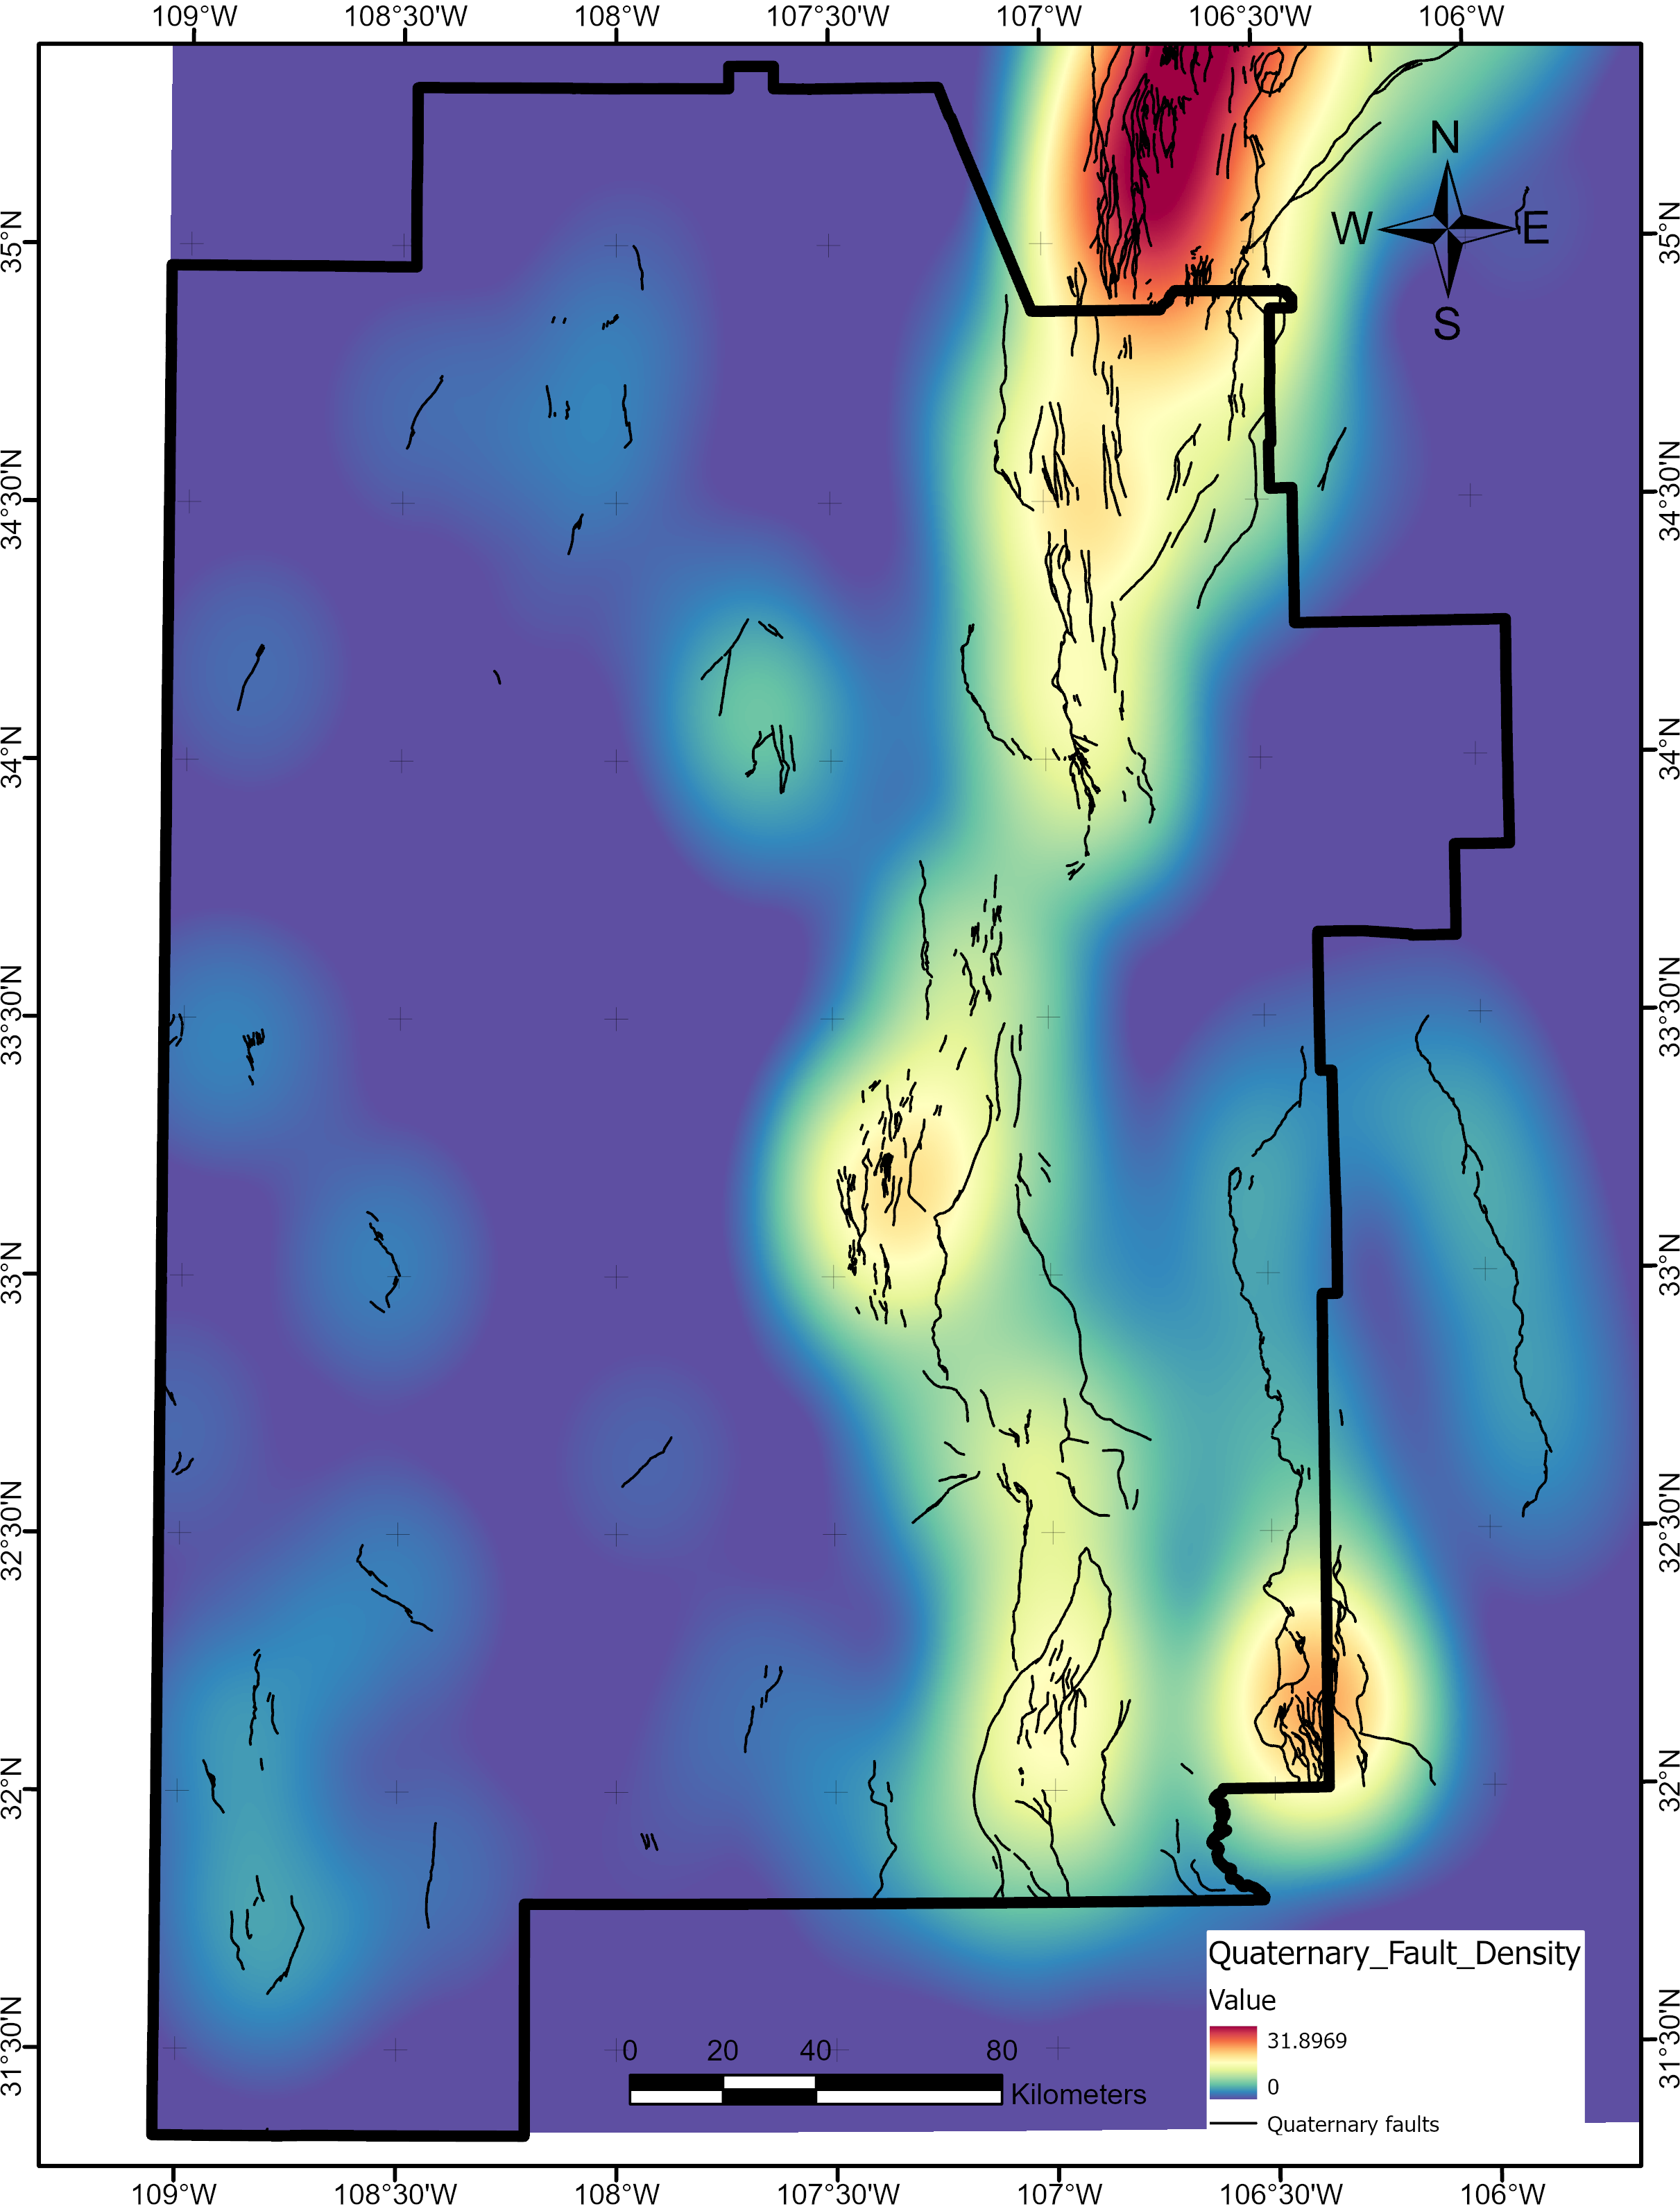
\includegraphics[scale=.50]{templates/images/Figure-QFaultDensity.png}
\caption[Quaternary fault density data layer]{Quaternary fault density data layer. Units are in degrees/square degress. Black lines show the fault polyline data set archived by \protect\citet{bielicki_hydrogeolgic_2015}.}.
\label{fig:feat_qfaults}
\end{figure}

\subsubsection{Silica Geothermometer Temperature}

Silica concentration data from across the study area were compiled by \citet{bielicki_hydrogeolgic_2015}, and converted to reservoir temperatures using the Fournier chalcedony geothermometer relationship \citep{fournier_chemical_1977}. These data were downloaded from the PFA OpenEI submission \citep{kelley_geothermal_2015} and merged together using ArcGIS and Python to create a single dataframe of 7259 measurements, all within the broader Extent Polygon bounds to avoid surface creation edge effects within the tighter AOI. As described for the Boron concentration data layer, attempts to model Si geothermometer estimates using Gaussian Processes provided unsatisfactory results. Instead, the final layer was generated using the ArcGIS \textit{Empirical Bayes Kriging} routine. Selected parameters include: Empirical data transformation type, a maximum of 100 points in each local model, 100 simulated semivariograms with K-Bessel model type, and a standard circular search neighborhood with a radius of 1.1957 (auto-generated), minimum of 10 neighbors, and maximum of 15 neighbors. The output grid cell size was set to 0.01 degrees. All coincident data was included in the calculation, so any overlapping measurements were considered in generating the final layer (Figure \ref{fig:feat_si_temp}).

\begin{figure}[!htp]
\centering
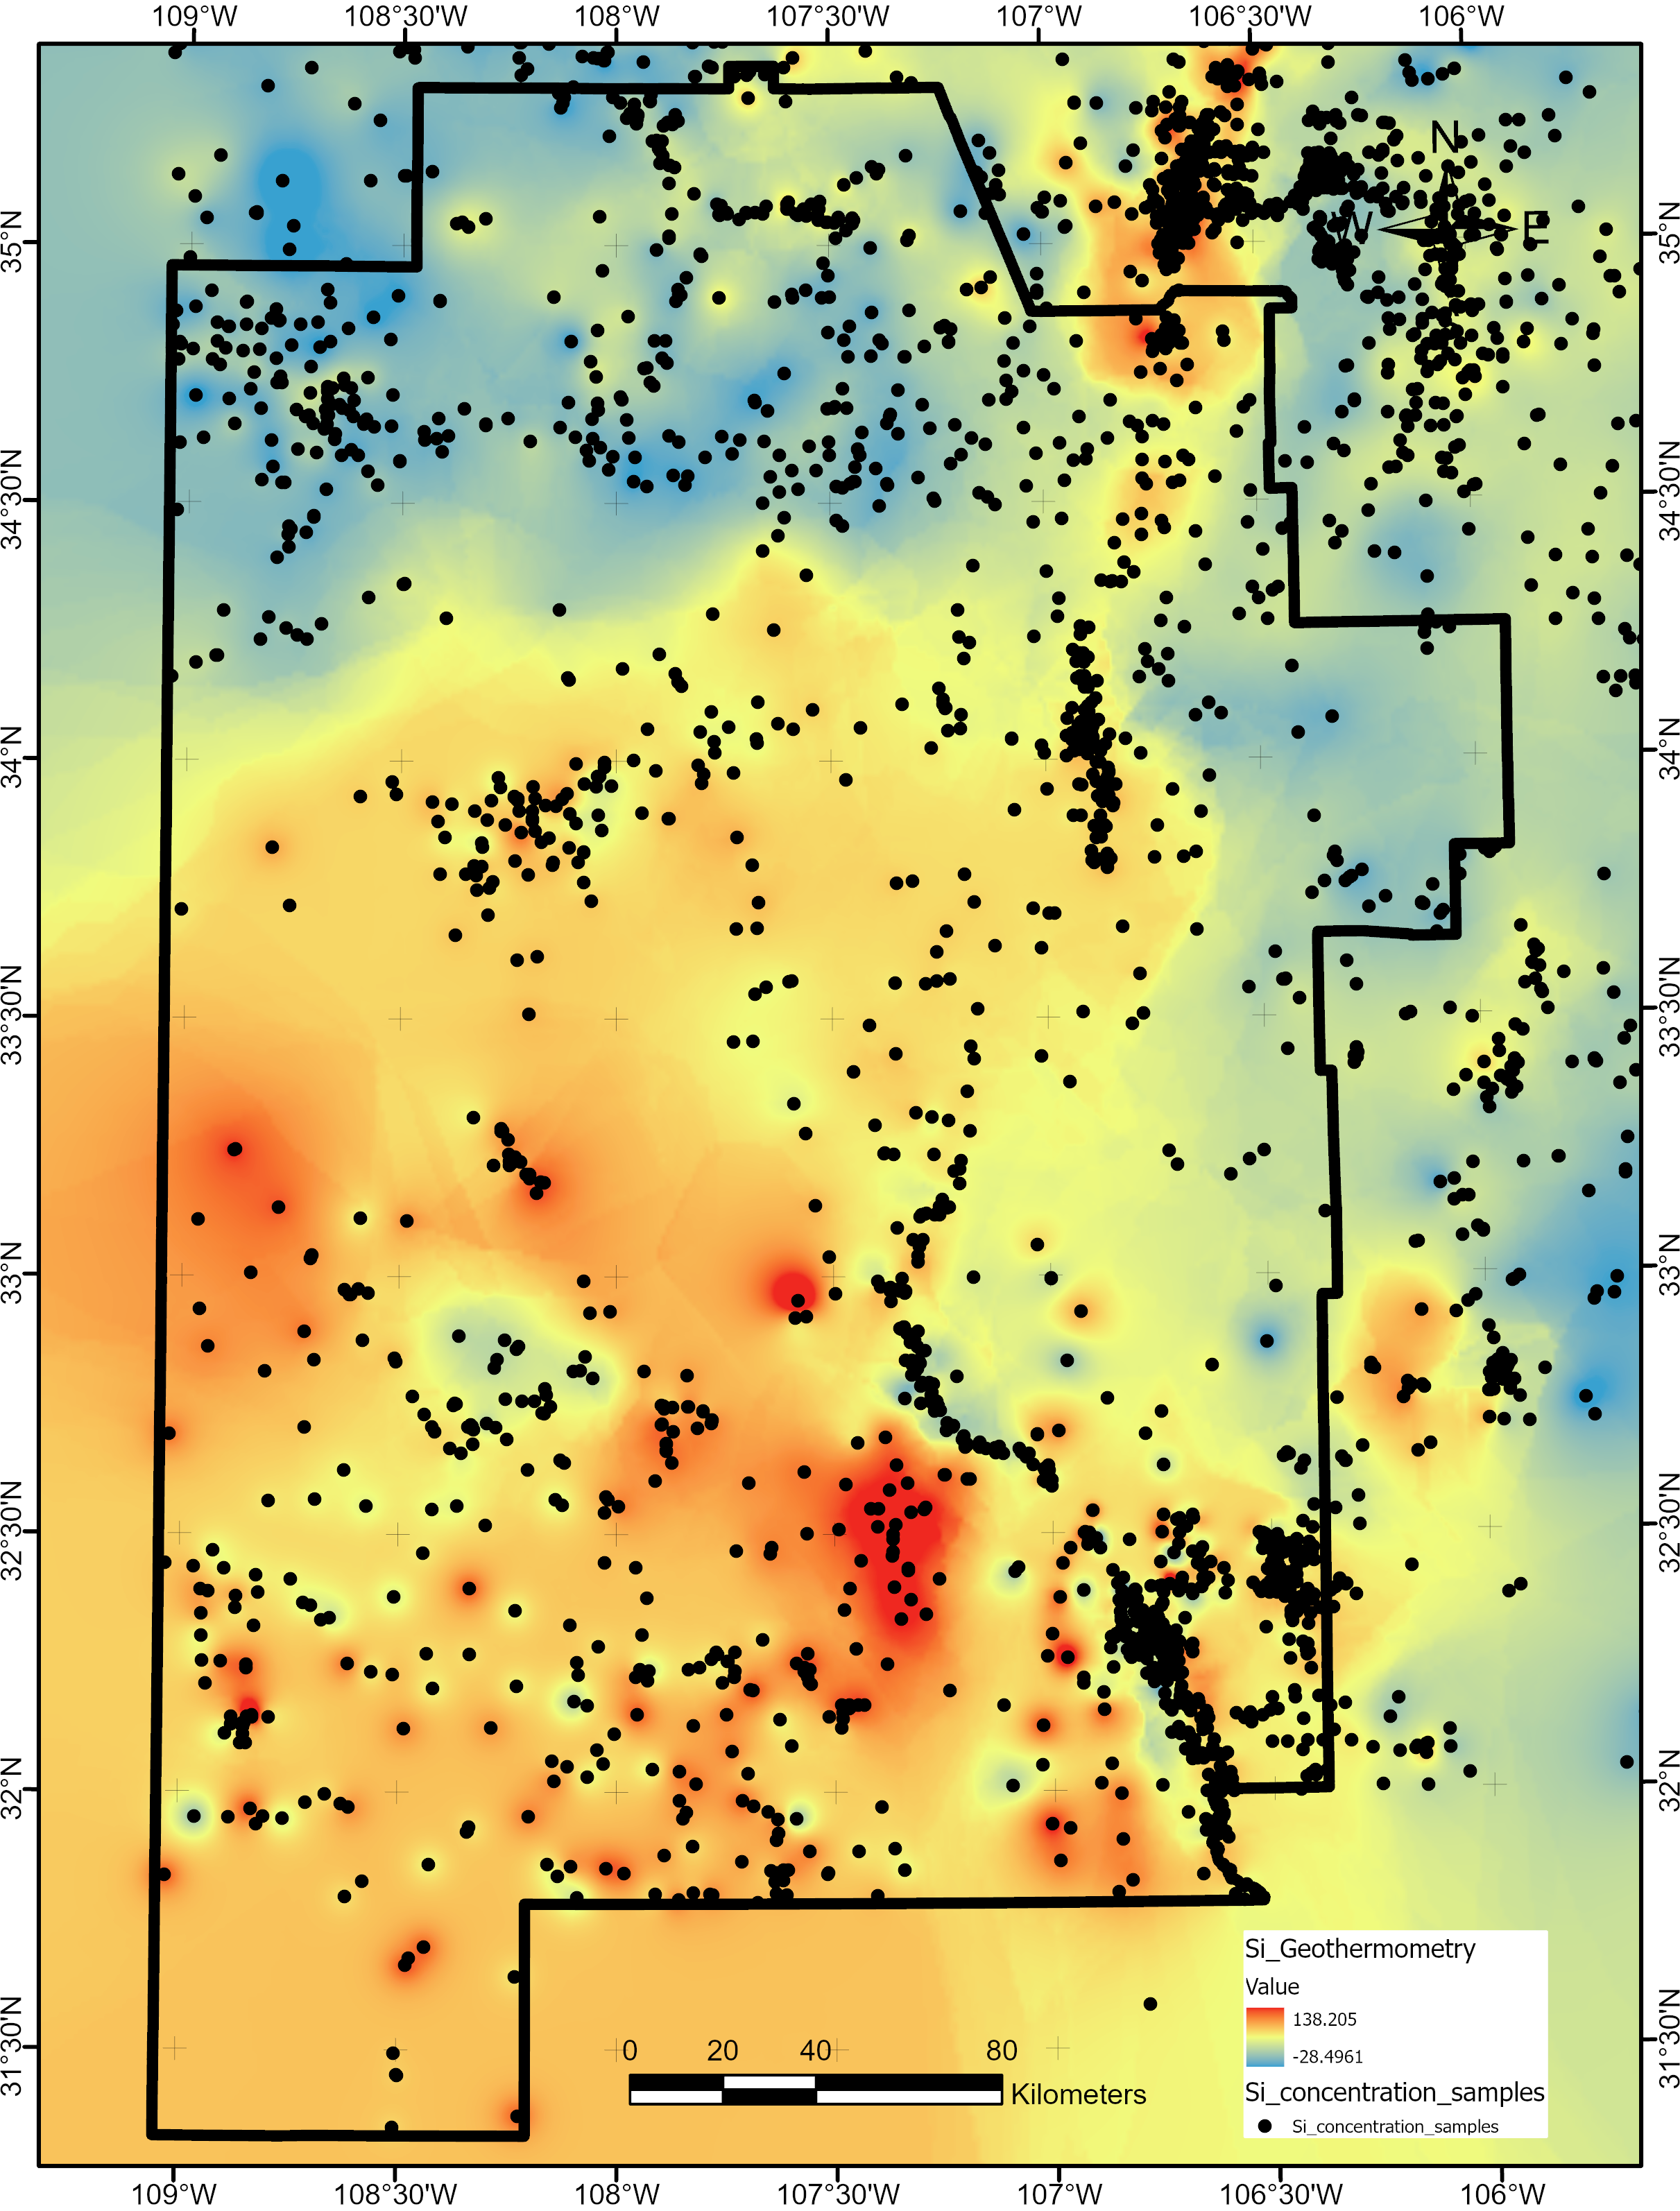
\includegraphics[scale=.50]{templates/images/Figure-SiTemp.png}
\caption[Silica geothermometer temperature data layer]{Chalcedony geothermometer data layer. Units are in degrees C. Black dots indicate locations where silica concentration was sampled, as collected by \protect\citet{bielicki_hydrogeolgic_2015}}.
\label{fig:feat_si_temp}
\end{figure}

\subsubsection{Water Table Depth}

\citeauthor{bielicki_hydrogeolgic_2015} (\citeyear{bielicki_hydrogeolgic_2015}) mapped the depth to water table using data from the USGS and several additional sources. This raster was downloaded from their OpenEI submission \citep{kelley_geothermal_2015} and imported into ArcGIS. Data gaps between the raster extent and AOI polygon to the south and the east necessitated extrapolation of the layer, so ArcGIS \textit{Empirical Bayes Kriging} was applied to fill in the missing edge values. After some trial-and-error, the chosen parameter values for the final layer (Figure \ref{fig:feat_wtdepth}) include an output cell size of 0.01, Empirical data transformation type, a maximum of 100 points in each local model, 100 simulated semivariograms with Exponential model type, and a standard circular search neighborhood with a radius of 1.2652 (auto-generated), minimum of 10 neighbors, and maximum of 15 neighbors.

\begin{figure}[!htp]
\centering
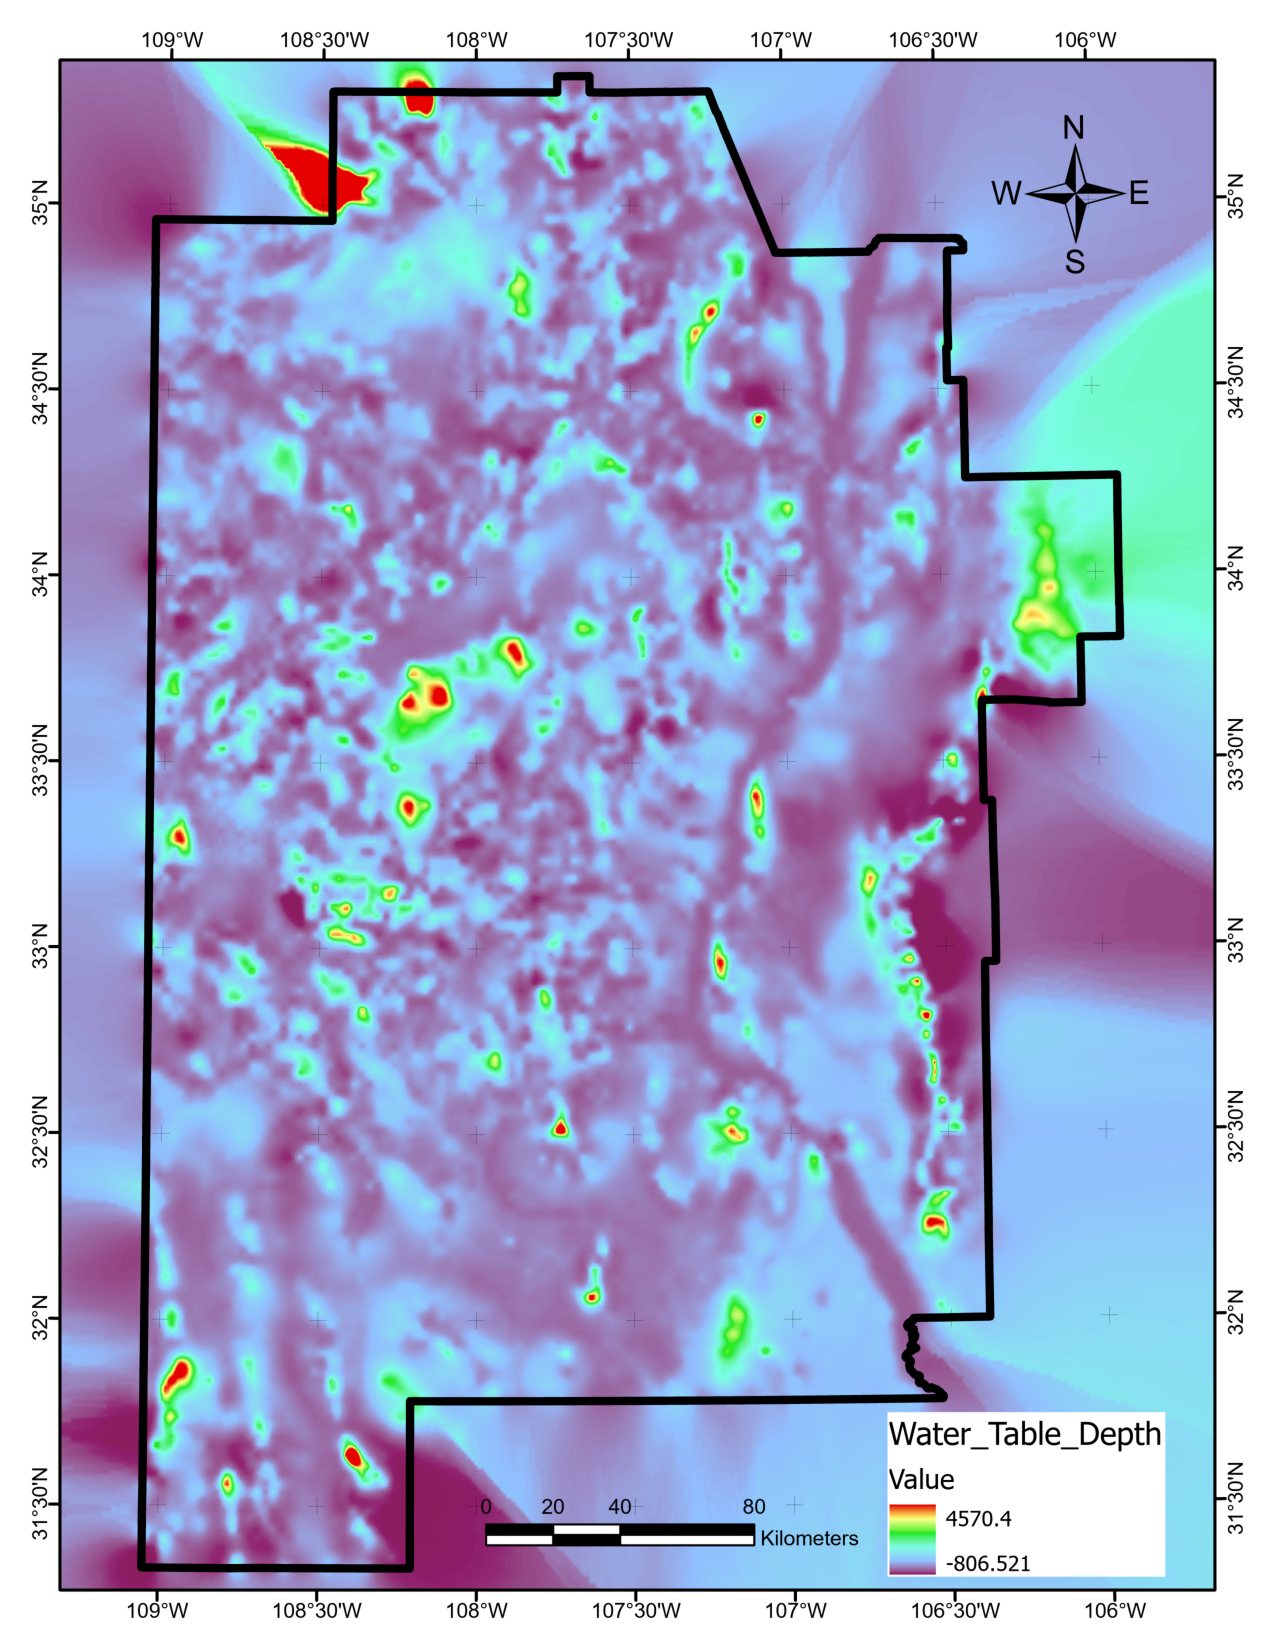
\includegraphics[scale=.50]{Figure-WTDepth}
\caption[Water table depth data layer]{Water table depth data layer. Units in feet. Adapted from raster created by \protect\citep{bielicki_hydrogeolgic_2015}.}
\label{fig:feat_wtdepth}
\end{figure}